% Options for packages loaded elsewhere
\PassOptionsToPackage{unicode}{hyperref}
\PassOptionsToPackage{hyphens}{url}
%
\documentclass[
  letterpaper,
]{scrbook}

\usepackage{amsmath,amssymb}
\usepackage{iftex}
\ifPDFTeX
  \usepackage[T1]{fontenc}
  \usepackage[utf8]{inputenc}
  \usepackage{textcomp} % provide euro and other symbols
\else % if luatex or xetex
  \usepackage{unicode-math}
  \defaultfontfeatures{Scale=MatchLowercase}
  \defaultfontfeatures[\rmfamily]{Ligatures=TeX,Scale=1}
\fi
\usepackage{lmodern}
\ifPDFTeX\else  
    % xetex/luatex font selection
\fi
% Use upquote if available, for straight quotes in verbatim environments
\IfFileExists{upquote.sty}{\usepackage{upquote}}{}
\IfFileExists{microtype.sty}{% use microtype if available
  \usepackage[]{microtype}
  \UseMicrotypeSet[protrusion]{basicmath} % disable protrusion for tt fonts
}{}
\makeatletter
\@ifundefined{KOMAClassName}{% if non-KOMA class
  \IfFileExists{parskip.sty}{%
    \usepackage{parskip}
  }{% else
    \setlength{\parindent}{0pt}
    \setlength{\parskip}{6pt plus 2pt minus 1pt}}
}{% if KOMA class
  \KOMAoptions{parskip=half}}
\makeatother
\usepackage{xcolor}
\usepackage{soul}
\setlength{\emergencystretch}{3em} % prevent overfull lines
\setcounter{secnumdepth}{5}
% Make \paragraph and \subparagraph free-standing
\ifx\paragraph\undefined\else
  \let\oldparagraph\paragraph
  \renewcommand{\paragraph}[1]{\oldparagraph{#1}\mbox{}}
\fi
\ifx\subparagraph\undefined\else
  \let\oldsubparagraph\subparagraph
  \renewcommand{\subparagraph}[1]{\oldsubparagraph{#1}\mbox{}}
\fi

\usepackage{color}
\usepackage{fancyvrb}
\newcommand{\VerbBar}{|}
\newcommand{\VERB}{\Verb[commandchars=\\\{\}]}
\DefineVerbatimEnvironment{Highlighting}{Verbatim}{commandchars=\\\{\}}
% Add ',fontsize=\small' for more characters per line
\usepackage{framed}
\definecolor{shadecolor}{RGB}{241,243,245}
\newenvironment{Shaded}{\begin{snugshade}}{\end{snugshade}}
\newcommand{\AlertTok}[1]{\textcolor[rgb]{0.68,0.00,0.00}{#1}}
\newcommand{\AnnotationTok}[1]{\textcolor[rgb]{0.37,0.37,0.37}{#1}}
\newcommand{\AttributeTok}[1]{\textcolor[rgb]{0.40,0.45,0.13}{#1}}
\newcommand{\BaseNTok}[1]{\textcolor[rgb]{0.68,0.00,0.00}{#1}}
\newcommand{\BuiltInTok}[1]{\textcolor[rgb]{0.00,0.23,0.31}{#1}}
\newcommand{\CharTok}[1]{\textcolor[rgb]{0.13,0.47,0.30}{#1}}
\newcommand{\CommentTok}[1]{\textcolor[rgb]{0.37,0.37,0.37}{#1}}
\newcommand{\CommentVarTok}[1]{\textcolor[rgb]{0.37,0.37,0.37}{\textit{#1}}}
\newcommand{\ConstantTok}[1]{\textcolor[rgb]{0.56,0.35,0.01}{#1}}
\newcommand{\ControlFlowTok}[1]{\textcolor[rgb]{0.00,0.23,0.31}{#1}}
\newcommand{\DataTypeTok}[1]{\textcolor[rgb]{0.68,0.00,0.00}{#1}}
\newcommand{\DecValTok}[1]{\textcolor[rgb]{0.68,0.00,0.00}{#1}}
\newcommand{\DocumentationTok}[1]{\textcolor[rgb]{0.37,0.37,0.37}{\textit{#1}}}
\newcommand{\ErrorTok}[1]{\textcolor[rgb]{0.68,0.00,0.00}{#1}}
\newcommand{\ExtensionTok}[1]{\textcolor[rgb]{0.00,0.23,0.31}{#1}}
\newcommand{\FloatTok}[1]{\textcolor[rgb]{0.68,0.00,0.00}{#1}}
\newcommand{\FunctionTok}[1]{\textcolor[rgb]{0.28,0.35,0.67}{#1}}
\newcommand{\ImportTok}[1]{\textcolor[rgb]{0.00,0.46,0.62}{#1}}
\newcommand{\InformationTok}[1]{\textcolor[rgb]{0.37,0.37,0.37}{#1}}
\newcommand{\KeywordTok}[1]{\textcolor[rgb]{0.00,0.23,0.31}{#1}}
\newcommand{\NormalTok}[1]{\textcolor[rgb]{0.00,0.23,0.31}{#1}}
\newcommand{\OperatorTok}[1]{\textcolor[rgb]{0.37,0.37,0.37}{#1}}
\newcommand{\OtherTok}[1]{\textcolor[rgb]{0.00,0.23,0.31}{#1}}
\newcommand{\PreprocessorTok}[1]{\textcolor[rgb]{0.68,0.00,0.00}{#1}}
\newcommand{\RegionMarkerTok}[1]{\textcolor[rgb]{0.00,0.23,0.31}{#1}}
\newcommand{\SpecialCharTok}[1]{\textcolor[rgb]{0.37,0.37,0.37}{#1}}
\newcommand{\SpecialStringTok}[1]{\textcolor[rgb]{0.13,0.47,0.30}{#1}}
\newcommand{\StringTok}[1]{\textcolor[rgb]{0.13,0.47,0.30}{#1}}
\newcommand{\VariableTok}[1]{\textcolor[rgb]{0.07,0.07,0.07}{#1}}
\newcommand{\VerbatimStringTok}[1]{\textcolor[rgb]{0.13,0.47,0.30}{#1}}
\newcommand{\WarningTok}[1]{\textcolor[rgb]{0.37,0.37,0.37}{\textit{#1}}}

\providecommand{\tightlist}{%
  \setlength{\itemsep}{0pt}\setlength{\parskip}{0pt}}\usepackage{longtable,booktabs,array}
\usepackage{calc} % for calculating minipage widths
% Correct order of tables after \paragraph or \subparagraph
\usepackage{etoolbox}
\makeatletter
\patchcmd\longtable{\par}{\if@noskipsec\mbox{}\fi\par}{}{}
\makeatother
% Allow footnotes in longtable head/foot
\IfFileExists{footnotehyper.sty}{\usepackage{footnotehyper}}{\usepackage{footnote}}
\makesavenoteenv{longtable}
\usepackage{graphicx}
\makeatletter
\def\maxwidth{\ifdim\Gin@nat@width>\linewidth\linewidth\else\Gin@nat@width\fi}
\def\maxheight{\ifdim\Gin@nat@height>\textheight\textheight\else\Gin@nat@height\fi}
\makeatother
% Scale images if necessary, so that they will not overflow the page
% margins by default, and it is still possible to overwrite the defaults
% using explicit options in \includegraphics[width, height, ...]{}
\setkeys{Gin}{width=\maxwidth,height=\maxheight,keepaspectratio}
% Set default figure placement to htbp
\makeatletter
\def\fps@figure{htbp}
\makeatother
\newlength{\cslhangindent}
\setlength{\cslhangindent}{1.5em}
\newlength{\csllabelwidth}
\setlength{\csllabelwidth}{3em}
\newlength{\cslentryspacingunit} % times entry-spacing
\setlength{\cslentryspacingunit}{\parskip}
\newenvironment{CSLReferences}[2] % #1 hanging-ident, #2 entry spacing
 {% don't indent paragraphs
  \setlength{\parindent}{0pt}
  % turn on hanging indent if param 1 is 1
  \ifodd #1
  \let\oldpar\par
  \def\par{\hangindent=\cslhangindent\oldpar}
  \fi
  % set entry spacing
  \setlength{\parskip}{#2\cslentryspacingunit}
 }%
 {}
\usepackage{calc}
\newcommand{\CSLBlock}[1]{#1\hfill\break}
\newcommand{\CSLLeftMargin}[1]{\parbox[t]{\csllabelwidth}{#1}}
\newcommand{\CSLRightInline}[1]{\parbox[t]{\linewidth - \csllabelwidth}{#1}\break}
\newcommand{\CSLIndent}[1]{\hspace{\cslhangindent}#1}

\makeatletter
\makeatother
\makeatletter
\@ifpackageloaded{bookmark}{}{\usepackage{bookmark}}
\makeatother
\makeatletter
\@ifpackageloaded{caption}{}{\usepackage{caption}}
\AtBeginDocument{%
\ifdefined\contentsname
  \renewcommand*\contentsname{Table of contents}
\else
  \newcommand\contentsname{Table of contents}
\fi
\ifdefined\listfigurename
  \renewcommand*\listfigurename{List of Figures}
\else
  \newcommand\listfigurename{List of Figures}
\fi
\ifdefined\listtablename
  \renewcommand*\listtablename{List of Tables}
\else
  \newcommand\listtablename{List of Tables}
\fi
\ifdefined\figurename
  \renewcommand*\figurename{Figure}
\else
  \newcommand\figurename{Figure}
\fi
\ifdefined\tablename
  \renewcommand*\tablename{Table}
\else
  \newcommand\tablename{Table}
\fi
}
\@ifpackageloaded{float}{}{\usepackage{float}}
\floatstyle{ruled}
\@ifundefined{c@chapter}{\newfloat{codelisting}{h}{lop}}{\newfloat{codelisting}{h}{lop}[chapter]}
\floatname{codelisting}{Listing}
\newcommand*\listoflistings{\listof{codelisting}{List of Listings}}
\makeatother
\makeatletter
\@ifpackageloaded{caption}{}{\usepackage{caption}}
\@ifpackageloaded{subcaption}{}{\usepackage{subcaption}}
\makeatother
\makeatletter
\@ifpackageloaded{tcolorbox}{}{\usepackage[skins,breakable]{tcolorbox}}
\makeatother
\makeatletter
\@ifundefined{shadecolor}{\definecolor{shadecolor}{rgb}{.97, .97, .97}}
\makeatother
\makeatletter
\makeatother
\makeatletter
\makeatother
\ifLuaTeX
  \usepackage{selnolig}  % disable illegal ligatures
\fi
\IfFileExists{bookmark.sty}{\usepackage{bookmark}}{\usepackage{hyperref}}
\IfFileExists{xurl.sty}{\usepackage{xurl}}{} % add URL line breaks if available
\urlstyle{same} % disable monospaced font for URLs
\hypersetup{
  pdftitle={Outils de recherche en sciences sociales numériques},
  pdfauthor={Chaire de leadership en enseignement des sciences sociales numériques (CLESSN)},
  hidelinks,
  pdfcreator={LaTeX via pandoc}}

\title{Outils de recherche en sciences sociales numériques}
\author{Chaire de leadership en enseignement des sciences sociales
numériques (CLESSN)}
\date{2023-08-24}

\begin{document}
\frontmatter
\maketitle
\ifdefined\Shaded\renewenvironment{Shaded}{\begin{tcolorbox}[sharp corners, boxrule=0pt, interior hidden, borderline west={3pt}{0pt}{shadecolor}, enhanced, breakable, frame hidden]}{\end{tcolorbox}}\fi

\renewcommand*\contentsname{Table of contents}
{
\setcounter{tocdepth}{2}
\tableofcontents
}
\mainmatter
\bookmarksetup{startatroot}

\hypertarget{avant-propos}{%
\chapter*{Avant-propos}\label{avant-propos}}
\addcontentsline{toc}{chapter}{Avant-propos}

\markboth{Avant-propos}{Avant-propos}

Ceci est un exemple de citation Adcock and Collier (2001) .

\bookmarksetup{startatroot}

\hypertarget{introduction}{%
\chapter*{Introduction}\label{introduction}}
\addcontentsline{toc}{chapter}{Introduction}

\markboth{Introduction}{Introduction}

\bookmarksetup{startatroot}

\hypertarget{trois-duxe9fis-pour-une-contribution-aux-sciences-sociales-numuxe9riques}{%
\chapter{Trois défis pour une contribution aux sciences sociales
numériques}\label{trois-duxe9fis-pour-une-contribution-aux-sciences-sociales-numuxe9riques}}

Ce premier chapitre n'est sans doute pas le plus excitant. Il ne
comprend ni graphique ni exercice. Il s'ancre dans la réflexion
théorique plutôt que dans la pratique méthodologique. Habituellement,
c'est la partie que l'on ignore, celle que l'on saute pour passer aux «
choses sérieuses ». Amateur de « choses sérieuses »? Bonne nouvelle! Cet
ouvrage en est rempli. Tout comme la carrière qui s'offre à vous si vous
choisissez de poursuivre dans l'étude des sciences sociales numériques.

En 2020, le monde est numérique, et rien ne semble présager un
inversement de la tendance. Au contraire, celle-ci risque plutôt de
s'accélérer. La pandémie de la COVID-19 a offert quelques-uns des
meilleurs exemples de cette tendance: télétravail généralisé, école
numérique, livraison en ligne, mobilisation via les réseaux sociaux,
intelligences artificielles pour le dépistage de fausses nouvelles et
application mobile pour tracer les déplacements et freiner les
pandémies. L'avenir est au numérique. Pour les jeunes chercheurs en
sciences sociales, cela équivaut à une montagne de «choses sérieuses».

Dans ce contexte, il ne fait aucun doute que votre carrière sera
passionnante. Si vous n'en êtes pas déjà convaincu, ce livre vous
fournira une panoplie d'exemples de vos nombreuses possibilités. De
l'analyse textuelle dans les médias aux sondages en ligne de milliers
d'individus, en passant par l'extraction de données massives des sites
web ou à l'analyse de larges réseaux de communication, vous trouverez
assurément des défis à la hauteur de vos aspirations.

Devant ce déluge de données numériques, le jeune chercheur peut avoir
l'impression qu'il est possible, voire permis de tout faire.
Entendons-nous bien: c'est presque le cas. Tous les jours, vous aurez
des idées de projets plus invraisemblables les unes que les autres. Avec
vos nouveaux outils, plusieurs de ces idées n'auront aucun problème à se
réaliser. Le véritable problème surviendra peut-être le jour où sera
négligée la réflexion théorique. La réflexion au cœur même de ce
chapitre. Rappelez-vous: c'est ce chapitre que vous avez considéré
sauter, au départ!

En fait, il serait surprenant que vous ne soyez pas happés, très tôt
dans vos études, à des limites fondamentales à votre travail. Dans cet
ouvrage, nous les appelleront « défis ». Nous ne parlons pas ici de
données manquantes ou d'accès restreints à l'information. Il s'agit de
défis beaucoup plus élémentaires. Ils se comptent au nombre de trois et
sont à la base de toute réflexion préalable à la recherche en science
sociales numériques. Ils sont:

\begin{enumerate}
\def\labelenumi{\arabic{enumi}.}
\tightlist
\item
  Le défi technique;
\item
  Le défi théorique;
\item
  Le défi éthique.
\end{enumerate}

Sachez une chose: ces défis sont présents dans toutes les grandes
branches de la science, c'est-à-dire lors de la recherche, lors de la
diffusion des résultats et lors de l'enseignement. Que vous comptiez
opérer dans l'une, dans l'autre ou dans toutes ces branches, une bonne
compréhension des trois défis permettra de limiter les risques d'impair,
mais surtout d'élargir l'univers de vos possibles.

\hypertarget{duxe9fi-1-linuxe9vitable-duxe9fi-technique.}{%
\section{Défi \#1: l'inévitable défi
technique.}\label{duxe9fi-1-linuxe9vitable-duxe9fi-technique.}}

Le premier défi est technique, lié à l'extraction et à l'analyse des
données numériques. Il nécessite l'apprentissage et le développement des
méthodologies. Avec R dans sa poche, ce défi est hautement simplifié. R
permet de penser autrement les possibilités de recherche, et de
travailler avec des outils tels que \emph{Shiny}, pour la création
instantanée d'applications web interactives ou \emph{Mechanical Turk},
pour la mise en ligne de micro-tâches (\emph{crowdsourcing}) à réaliser
à faible coût par des volontaires. R facilite également la réalisation
de revues de la portée de la littérature (\emph{scoping review}), une
technique permettant de cartographier la littérature scientifique dans
un champ donné.

Les données massives nous entourent. Que ce soit au travers de milliers
de sondages croisés, via les médias sociaux ou à l'intérieur des
archives gouvernementales en ligne, il est plus facile que jamais de
rassembler de grandes quantités d'information. Le défi demeure toutefois
complexe lorsque vient le temps d'extraire et d'analyser ces données
afin de contribuer à la connaissance scientifique.

Déjà, cet ouvrage offre une base solide sur laquelle développer vos
méthodes. Celles-ci sont de plus en plus simples à apprendre et à
appliquer, notamment grâce aux réseaux de collaboration en ligne.
Aujourd'hui, une question peut rapidement être répondue après une
recherche sur Google. \emph{Stack Overflow} est un site Web dédié à
l'entraide entre programmeurs. Vous le trouverez hautement utile.

Si les méthodologies sont plus nombreuses, efficaces et simples que
jamais, beaucoup restent encore à faire pour permettre la transparence
et l'accessibilité des données publiques, la collaboration entre
chercheurs et l'optimisation des outils d'extractions de données. Le
cœur du défi technique réside dans l'amélioration des outils utiles et
nécessaires aux chercheurs.

En effet, après l'apprentissage des méthodes disponibles à l'heure
actuelle, vous pourrez rapidement contribuer à leur optimisation. La
beauté d'un logiciel libre comme R est qu'il vous est possible de
développer de nouvelles méthodes pour faciliter la recherche, pour
ensuite partager ces trouvailles avec le monde entier. Sur R, vous
pourrez construire des fonctions qui accéléreront votre travail. Le
développement de quatre ou cinq fonctions pourrait ensuite faire l'objet
d'un tout nouveau « package », que vous partagerez en ligne à vos pairs
scientifiques.

Tous les jours, de nouveaux packages R sont développés et mis en ligne.
Des dizaines existent simplement pour réaliser de l'analyse textuelle
automatisée, une méthodologie qui permet l'étude quantitative de large
corpus de textes. Plusieurs de ces packages, comme «Quanteda»,
«Topicmodels», ou ceux de la «Tidyverse» sont hautement performants, et
en constante amélioration.

Il est à la portée de toute chercheuse et de tout chercheur de
participer à la bonification des outils et à l'avancement des
méthodologies. C'est la réponse attendu au défi technique.

\hypertarget{duxe9fi-2-le-nuxe9cessaire-duxe9fi-thuxe9orique.}{%
\section{Défi \#2: le nécessaire défi
théorique.}\label{duxe9fi-2-le-nuxe9cessaire-duxe9fi-thuxe9orique.}}

\begin{itemize}
\tightlist
\item
  Nécessite une formation selon les principaux travaux scientifiques qui
  étudient l'impact des données numériques sur les théories en sciences
  sociales:

  \begin{itemize}
  \tightlist
  \item
    On ne doit pas réinventer la roue à chaque article scientifique;
  \item
    Comment intégrer nos travaux à la littérature actuelle?;
  \item
    Comment faire progresser cette littérature? Démontrer l'impact des
    données numériques sur les théories existantes;
  \item
    Exemple: le nationalisme: peut-on mesurer le nationalisme au travers
    des médias sociaux? Si oui, comment cela peut-il contribuer à la
    littérature sur le nationalisme?
  \end{itemize}
\end{itemize}

\hypertarget{duxe9fi-3-luxe9pineux-duxe9fi-uxe9thique.}{%
\section{Défi \#3: l'épineux défi
éthique.}\label{duxe9fi-3-luxe9pineux-duxe9fi-uxe9thique.}}

\begin{itemize}
\tightlist
\item
  Autour des questions de l'effet de l'ère numérique sur la
  confidentialité, la sécurité informatique, le consentement et le droit
  des sujets secondaires:

  \begin{itemize}
  \tightlist
  \item
    Le numérique offre beaucoup d'opportunité tout à fait légale, mais
    pas nécessairement éthique;
  \item
    Nécessaire d'encourager la réflexion par rapport aux défis humains
    entourant l'utilisation des nouvelles données numériques;
  \item
    Comment utiliser ces données pour améliorer les vies, sans brimer
    les libertés individuelles?;
  \item
    Exemple: intelligence artificielle (machine learning): Le milieu
    académique est loin d'être seul à s'intéresser à la grande quantité
    d'information disponible. Les partis politiques, les agences de
    marketing et bien d'autres organisations utilisent ces informations
    à des fins de victoires, ou de ventes.
  \end{itemize}
\end{itemize}

\hypertarget{conclusion-de-cette-premiuxe8re-partie-du-chapitre}{%
\section{Conclusion de cette première partie du
chapitre}\label{conclusion-de-cette-premiuxe8re-partie-du-chapitre}}

\begin{itemize}
\tightlist
\item
  Au travers des nouveaux apprentissages et des exemples qui sont
  offerts dans ce livre, le lecteur est encouragé à se poser ces 3
  questions:
\end{itemize}

\begin{enumerate}
\def\labelenumi{\arabic{enumi}.}
\tightlist
\item
  D'abord, comment puis-je utiliser ces nouveaux outils pour faire
  progresser les méthodologies de recherche actuelles?
\item
  Ensuite, comment puis-je utiliser ces nouveaux outils pour contribuer
  à l'avancement des théories de mes champs de recherche?
\item
  Enfin, comment puis-je utiliser ces nouveaux outils pour exercer un
  impact positif sur mes semblables?
\end{enumerate}

\hypertarget{comment-les-donnuxe9es-massives-affectent-elles-les-sciences-sociales-changements-actuels-et-quelques-ruxe9flexions-sur-lavenir}{%
\section{Comment les données massives affectent-elles les sciences
sociales? Changements actuels et quelques réflexions sur
l'avenir}\label{comment-les-donnuxe9es-massives-affectent-elles-les-sciences-sociales-changements-actuels-et-quelques-ruxe9flexions-sur-lavenir}}

L'apparition des données massives (\emph{big data}) dans le paysage
technologique représente un de ces cas de plus en plus commun de
phénomène hautement technique dont les effets politiques et sociaux sont
remarquables. La discussion publique s'est en effet rapidement emparée
du sujet, au point de transformer un moment technologique en phénomène
social. Les «~données massives~» se trouvent ainsi régulièrement
présentées dans l'espace public à la fois comme un moyen puissant de
développement et d'innovation technoscientifique, de même que comme une
menace à la stabilité de certaines normes sociales telles que la
confidentialité des informations privées. Il n'est d'ailleurs pas rare
que le discours public s'inquiète du danger que poseraient les données
massives à la séparation des sphères publique et privée (centrale à la
conception libérale du rôle de la politique qui structure la majorité
des débats sociaux) en amalgamant parfois de manière trop rapide l'objet
et l'utilisation qui en est faite. Toutefois, ce même discours public
s'emporte aussi rapidement à propos des gains technologiques monumentaux
réalisés par l'utilisation des données massives.

Dans le domaine des sciences sociales, les avancées dûes à l'utilisation
des données massives se font de plus en plus fréquentes et l'impact des
données massives dans le domaine de la recherche sociale est en ce sens
indéniable. Toutefois, d'un point de vue épistémologique, l'utilisation
des données massives en recherche en sciences sociales dans les
dernières années laisse plusieurs questions ouvertes dans son sillage.

Comment l'utilisation des données massives change-t-elle la pratique des
sciences sociales? Les données massives causeront-elles un changement de
paradigme scientifique? Quels impacts auront-elles sur les traditions
scientifiques dominantes (e.g., béhavioralisme, individualisme
méthodologique) en sciences sociales?

Ce chapitre ne prétend pas offrir de réponses définitives à ces
questions, mais plutôt des pistes de réflexion par le biais d'une
introduction critique à certains points relatifs aux impacts des données
massives sur la recherche en sciences sociales. Premièrement, je
présente une conceptualisation des données massives. Deuxièmement, je me
penche sur les impacts des données massives en sciences sociales et
souligne tout particulièrement comment elles affectent les enjeux de la
\emph{validité} interne et externe dans la domaine des sciences
sociales. Finalement, j'explore quelques pistes de réflexion sur
l'avenir des données massives en sciences sociales en analysant quelques
changements \emph{épistémologiques} que ces données pourraient
potentiellement entraîner.

\hypertarget{duxe9finition-des-donnuxe9es-massives}{%
\section{Définition des données
massives}\label{duxe9finition-des-donnuxe9es-massives}}

Ce qui définie les données massives comme concept est souvent mêlé avec
le phénomène social qui l'accompagne. Il est toutefois possible de
demêler le tout en distinguant trois approches conceptuelles des données
massives.

\begin{enumerate}
\def\labelenumi{\arabic{enumi}.}
\item
  Premièrement, les données massives représentent une (1)
  \textbf{\emph{quantité importante de points d'information}} qui
  varient selon la nature, le type, la source, etc. En ce sens, la
  distinction est simplement quantitative. Il s'agit d'une première
  dimension à la définition des données massives.
\item
  Deuxièmement, d'une perspective technique et technologique, les
  données massives constituent un (2) ensemble de
  \textbf{\emph{pratiques}} de collecte, de traitement et d'analyse de
  ces points d'information. Les données massives représentent donc une
  technique ou une méthode nouvelle de recherche.
\item
  Finalement, d'une perspective sociologique, les données massives
  représentent (3) un phénomène incorporant à la fois la dimension
  propre aux \textbf{\emph{développements technologiques, ainsi que les
  impacts sociétaux de ces développements}}~-- i.e., les risques à la
  confidentialité des données, les enjeux relatifs au consentement et à
  l'autorisation de collecte des informations, les innovations en
  intelligence artificielle, etc. Cette perspective souligne le
  caractère essentiellement social des données massives.
\end{enumerate}

Dans les domaines scientifiques et technologiques, la définition
courante donnée aux données massives intègre des éléments de ces trois
niveaux d'analyses en se référant à la composition et à la fonction des
données. Premièrement, la \emph{composition} des données massives est
généralement conceptualisée comme comprenant «~4V~»~: le volume, la
variété, la vélocité et la véracité. Cette conceptualisation jouie d'un
large consensus scientifique (Chen, Mao et Liu, 2014; Gandomi et Haider,
2015; Kitchin et McArdle 2016).

Par ailleurs, plusieurs chercheurs ont élargi cette définition de la
composition des données massives en y incluant, par exemple, la
variabilité et la valeur des points de données (CITE). Deuxièmement, la
\emph{fonction} des données massives comprend les innovations relatives
à l'optimisation, à la prise de décision et à l'approfondissement des
connaissances qui résultent de leur utilisation. Ces fonctions touchent
des domaines sociaux disparates, incluant le souci d'efficacité et de
rendement du secteur privé et public ainsi que la recherche scientifique
pure (Gartner 2012).

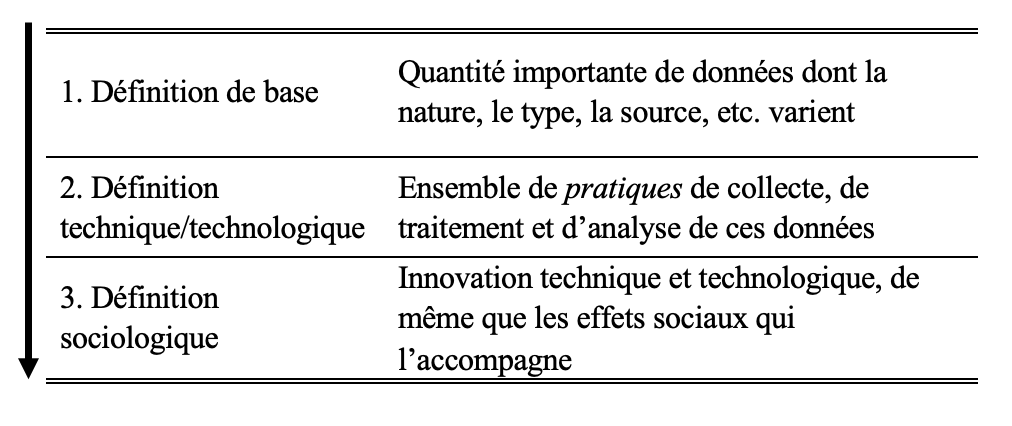
\includegraphics{images/Capture d’écran, le 2023-08-11 à 13.15.13.png}

\hypertarget{les-donnuxe9es-massives-et-les-sciences-sociales}{%
\section{Les données massives et les sciences
sociales}\label{les-donnuxe9es-massives-et-les-sciences-sociales}}

Dans le domaine des sciences sociales, les changements causés par
l'utilisation des données massives en recherche sont significatifs.
Plusieurs n'hésitent d'ailleurs pas à les qualifier de changement de
paradigme dans l'étude des phénomènes sociaux (Anderson 2008; Chandler
2015; Grimmer 2015; Kitchin 2014; Monroe et al.~2015). Dans le cas qui
nous intéresse, deux dimensions majeures méritent d'être abordées~: (1)
une première relative à la validité (interne et externe) des données
massives et (2) une seconde, plus large, relative au potentiel
changement de posture ou d'orientation épistémologique causé par
l'utilisation de ces données en recherche.

\hypertarget{la-validituxe9-de-la-mesure-en-sciences-sociales}{%
\section{La validité de la mesure en sciences
sociales}\label{la-validituxe9-de-la-mesure-en-sciences-sociales}}

La validité de la mesure constitue une exigence méthodologique centrale
à la recherche en sciences sociales.~Les scientifiques cherchent
effectivement à s'assurer que ce qui est mesuré -- par un sondage, une
entrevue, un thermostat ou tout autre outil de mesure -- constitue bel
et bien ce qui est supposé être mesuré. Adcock et Collier définissent
plus spécifiquement l'application de la validité de la mesure en
sciences sociales par le biais de «~scores (including the results of
qualitative classification) {[}that{]} meaningfully capture the ideas
contained in the corresponding concept.~» (2001~: 530)

Toutefois, les problèmes liés à la validité de la mesure sont nombreux
et ont une importance considérable. Dans l'étude des phénomènes sociaux
et humains, la validité de la mesure prend d'ailleurs une complexité
supplémentaire du fait que les données collectées par le biais d'une
mesure constituent le \emph{produit de l'observation} d'un phénomène
mais non pas le phénomène en soi. Ainsi, lorsque dans le contexte d'une
recherche on propose de mesurer l'humeur de l'opinion publique (le
phénomène en soi) sur un enjeu politique, on utilise généralement un
sondage qui a pour fonction de mesurer le pouls d'un échantillon de la
population d'intérêt (ce qui est réellement observé). Cependant, ce que
ce sondage mesure ne constitue pas tout à fait l'opinion publique
elle-même, mais plutôt un segment populationnel qui se veut
représentatif de l'humeur de l'opinion publique. Autrement dit, la
mesure et les données collectées ne représentent pas le phénomène --
l'opinion publique -- en soi.

On a déjà mentionné que la validité de la mesure a de l'importance
puisqu'elle garantit que ce qui est mesuré représente réellement ce
qu'on croit mesurer. Mais pour être plus spécifique, dans une approche
positiviste, la validité de la mesure se traduit généralement par une
logique de classification des valeurs attribuées aux différentes
manifestations distinctes d'un même phénomène. Par exemple, une mesure
de la démocratie comme celle proposée par \emph{Freedom House},
fréquemment utilisée en science politique, classifie les libertés
civiles et les droits politiques des états du monde par degré, de 1 à 7,
afin de construire un index allant d'autoritarisme complet à démocratie
parfaite. Les scores représentent, dans ce contexte, une mesure
artificielle, mais ordonnée et logique, des idées contenues dans le
concept de démocratie telles que libertés civiles et droits politiques.
On peut ainsi dire que le souci avec la validité de la mesure traverse
les connexions entre (1) le phénomène social étudié (la démocratie), (2)
son opérationnalisation (via les libertés civiles et droits politiques)
et (3) la méthode de mesure utilisée pour observer et classifier d'une
certaine façon le phénomène et les données qui en découlent (dans le cas
de \emph{Freedom House} des codeurs indépendants).

\hypertarget{la-validituxe9-des-donnuxe9es-massives}{%
\section{La validité des données
massives}\label{la-validituxe9-des-donnuxe9es-massives}}

En ce qui a trait aux données massives, la question de la validité de la
mesure constitue un défi nouveau. Les données massives ont en effet pour
avantage d'offrir aux chercheur.e.s soit de nouveaux phénomènes à
étudier, soit de nouvelles manifestations et nouvelles formes à des
phénomènes déjà étudiés. Les données massives permettent donc d'agrandir
la connaissance scientifique.

L'étude de King et al.~(2013) représente un cas éclairant de phénomène
social que que l'utilisation des données massives a rendu possible
d'étudier. En se basant sur la collecte de plus de 11 millions de
publications sur les réseaux sociaux chinois, King et al.~ont pu mesurer
la censure exercée par le gouvernement chinois sur les réseaux sociaux.
En utilisant des données massives nouvelles, King et al.~ont donc pu
observer une manifestation inédite de censure massive qui, sans de
telles données, serait probablement demeurer mal comprise d'une
perspective scientifique. Le nombre de recherches basées sur
l'utilisation des données massives similairement innovantes en sciences
sociales est par ailleurs en croissance constante (Beauchamp 2017; Bond
et al.~2012; Poirier et al.~2020).

Cependant, il faut aussi souligner que les données massives, de par leur
complexité, peuvent avoir pour désavantage d'embrouiller l'étude des
phénomènes sociaux. Les opportunités scientifiques liées aux données
massives s'accompagnent en effet de certaines difficultés
méthodologiques.

Aux nombres de ces difficultés, trois questions sont particulièrement
cruciales : (1) la validité interne, (2) la validité externe, et (3) la
question d'un changement de posture ou d'orientation épistémologique en
sciences sociales causé par les données massives.

\hypertarget{validituxe9-interne-des-donnuxe9es-massives}{%
\subsection{Validité interne des données
massives}\label{validituxe9-interne-des-donnuxe9es-massives}}

Premièrement, les données massives peuvent représenter un défi à la
validité interne des études en sciences sociales en rendant
\textbf{\emph{pragmatiquement difficile l'établissement d'un mécanisme
causal clair}}. Ce défi est notamment une conséquence du fait que la
plupart des données sont présentement issues d'un processus de
génération (\emph{data-generating process}) qui est hors du contrôle des
chercheur.e.s. Les données massives proviennent en effet habituellement
de sources diverses qui sont externes aux projets de recherche qui les
utilisent. Elles ne sont pas donc générées de manière aléatoire sous le
contrôle des chercheur.e.s.

Un des problèmes liés à cette situation consiste en ce qu'il est
difficile de garantir une source \emph{exogène} de variation par
laquelle les chercheur.e.s éliminent l'effet potentiel des facteurs
confondants (\emph{confounders}). La distribution aléatoire d'un
traitement et d'un contrôle (dans une expérience en laboratoire ou sur
le terrain) représente le standard le plus élevé permettant de fournir
cette source exogène de variation.

Pour le dire autrement, le défi de validité interne avec les données
massives constitue un enjeu relatif à la qualité des données. Ce n'est
évidemment pas un défi propre ou unique aux données massives. Ce défi
s'applique également aux autres types de données.

Cependant, dans l'état actuel des choses, le volume et la variété (2 des
4 V) des données massives (textuelles, numériques, vidéos, etc.) peuvent
miner la qualité de l'inférence causal entre un cause et une conséquence
que permet habituellement un processus contrôlé de génération des
données. En somme, la validité interne des données massives est une
fonction de la qualité de ces mêmes données.~

\hypertarget{validituxe9-externe-des-donnuxe9es-massives}{%
\subsection{Validité externe des données
massives}\label{validituxe9-externe-des-donnuxe9es-massives}}

Deuxièmement, les données massives représentent un défi plus important
pour la validité externe des recherches en sciences sociales (Tufekci
2014; Lazer et Radford 2017; Nagler et Tucker 2015). La préoccupation la
plus évidente concerne la \textbf{\emph{représentativité}} des données
massives collectées. Comme le souligne Lazer et Radford (2017), la
quantité ne permet pas de corriger pour la non-représentativité des
données. Les données massives sont ainsi soumises au même problème de
biais de sélection que les autres types de données observationnelles,
telle un sondage ou une série d'entrevues, traditionnellement utilisées
en sciences sociales.

Le cas célèbre de l'erreur de prédiction du \emph{Literary Digest} lors
de la campagne présidentielle américaine de 1936 illustre bien ce
problème récurrent. Le \emph{Literary Digest} a effectivement prédit à
tort la victoire de Alf Landon, le candidat du parti républicain, sur
Franklin D. Roosevelt, le candidat démocrate, parce que l'échantillon de
répondants utilisé par le \emph{Literary Digest} dans son sondage a
surrpresenté les électeurs plus aisés, traditionnellement plus
républicains, au détriment des électeurs moins aisés, plus généralement
proches du parti démocrate. Cette erreur de surreprésentation dans
l'échantillon est dûe au fait que le \emph{Literary Digest} a effectué
un échantillonnage basé sur les listes téléphoniques et le registre des
propriétaires de voitures, biaisant par le fait même l'échantillon au
détriment des électeurs plus pauvres ne possédant pas de téléphone ou
d'automobile mais qui constituaient un électorat favorable à Roosevelt
(Squire 1981).~Le biais de sélection du sondage a ainsi sous-estimé le
soutien populaire de Roosevelt de plus de 20\%.

Aujourd'hui, l'utilisation des données massives est soumise aux mêmes
risques méthodologiques. L'accumulation massive de données ne permet pas
de compenser pour la qualité des données. Les données massives, comme
les données plus traditionnelles, sont soumises aux conséquences
induites par le processus de génération des données (\emph{data
generating process}) comme un échantillonnage.

\hypertarget{donnuxe9es-expuxe9rimentales}{%
\subsection{Données expérimentales}\label{donnuxe9es-expuxe9rimentales}}

La question du \emph{processus de génération} des données est plus
claire quand on considère comment les \emph{données observationnelles}
et les \emph{données expérimentales} permettent d'effectuer des
\emph{inférences} de manière distincte.

Premièrement, les données massives ne peuvent pas résoudre les enjeux
liés aux inférences causalesou explicatives(Grimmer, 2015). En effet, le
processus de génération de données expérimentales assure idéalement la
validité de l'inférence causale sur l'ensemble de la population visée.
Cela prend plus spécifiquement la forme d'un processus de génération des
données au sein duquel les chercheur.e.s assurent la distribution
aléatoire du traitement entre les deux groupes traitement et contrôle,
garantissant par le fait même une source exogène de variation qui permet
d'éliminer l'endogénéité entre la variable indépendante (\emph{x}) et le
résidu (\emph{e}) et qui assure donc que l'effet observé n'est pas dû à
une variable confondante.

\hypertarget{donnuxe9es-observationnelles}{%
\subsection{Données
observationnelles}\label{donnuxe9es-observationnelles}}

En ce qui à trait aux données observationnelles, il y a deux points
importants. Premièrement, des méthodes d'inférence basées sur des
approches par «~design~» (\emph{design-based methods}) comme une méthode
de régression sur discontinuité, de variable instrumentale, etc. peuvent
également garantir des inférences explicatives et causales valides.
Elles nécessitent toutefois plusieurs postulats plus restrictifs dont
l'objectif est d'imiter ou de récréer, de la manière la plus fidèle
possible, une distribution aléatoire du traitement -- ce que la
litérature appelle un «~\emph{as-if random assignment}~» (Dunning,
2008).

Dans un contexte observationnel, les données massives peuvent donc
permettre d'augmenter la précision des estimations causales.
Effectivement, comme dans un modèle de régression linéaire, plus
l'échantillon est grand, plus l'estimation du coefficient (causal ou
probabiliste) est précise. Par exemple, un échantillon large dans un
modèle de régression sur discontinuité permet de restreindre la largeur
de bande autour du «~seuil~», garantissant ainsi une distribution
presque parfaitement aléatoire des données et une validité plus élevée à
l'estimation de l'effet causal.

Deuxièmement, un échantillon de données massives observationnelles
issues d'une plateforme comme Twitter ou Facebook peut fournir une
\emph{description} plus fine de certaines dynamiques sociales observées
sur les réseaux sociaux. Cependant, c'est la manière dont sont
collectées les données de cet échantillon de données massives qui
garantit la représentativité de l'échantillon (avec pour objectif un
biais de sélection = 0) et non pas la quantité de données. Généralement,
le biais d'un échantillon est une conséquence de la non-représentativité
des répondants -- dans notre exemple, les utilisateurs des médias
sociaux ne sont généralement pas représentatifs de la population
entière.

Dans un tel cas, des méthodes de pondération sur des données
observationnelles peuvent compenser pour la sur- ou la
sous-représentativité de sous-groupes dans un échantillon afin d'assurer
la validité de l'inférence entre échantillon et population. Les données
massives ont ici une importance puisqu'une pondération fiable nécessite
une quantité substantielle d'observations. Une pondération \emph{a
posteriori} sera donc plus fiable plus l'échantillon est grand. Les
données massives ont ainsi une valeur ajoutée afin d'établir des
inférences descriptives plus précises et sophistiquées.

\hypertarget{validituxe9-uxe9cologique-et-observation-par-sous-groupes}{%
\subsection{Validité écologique et observation par
sous-groupes}\label{validituxe9-uxe9cologique-et-observation-par-sous-groupes}}

Les données massives peuvent aussi jouer d'autres rôles importants
relatif à la validité externe. Premièrement, les données massives
facilitent effectivement la validité externe de certaines études en
accroissant la «~validité écologique~» (\emph{ecological validity}) des
tests expérimentaux, c'est-à-dire le réalisme de la situation
expérimentale (Grimmer, 2015~: 81). En effet, la variété des sources et
des formats de données permet aux chercheurs d'imiter plus concrètement
la réalité «~sur le terrain~» vécue par les participants aux études.

Deuxièmement, la quantité importante de données rend possible
l'observation d'effets précis, spécifiques et inédits par sous-groupes
(Grimmer 2015~: 81). Alors qu'auparavant la taille réduite des
échantillons ne permettait pas d'effectuer des inférences valides pour
des sous-groupes de la population -- les écart-types par sous-groupes
étaient trop grand, rendant difficile l'estimation précise d'un
paramètre comme la moyenne et impossible celle d'un coefficient --, la
taille énorme des échantillons permet aux chercheurs d'estimer des
paramètres qui étaient demeurés extrêmement imprécis jusqu'à
aujourd'hui. Notre compréhension des phénomènes sociaux s'en trouve par
le fait même approfondi de façon considérable.

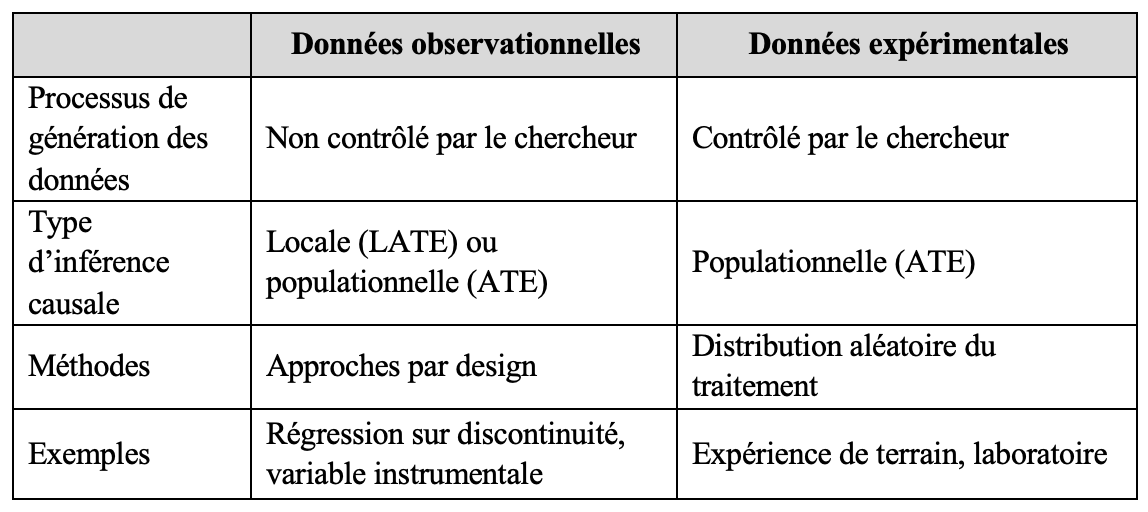
\includegraphics{images/Capture d’écran, le 2023-08-11 à 13.19.08.png}

\hypertarget{vers-le-futur-les-donnuxe9es-massives-effectueront-elles-un-changement-dans-la-posture-uxe9pistuxe9mologique-en-sciences-sociales}{%
\section{Vers le futur~: les données massives effectueront-elles un
changement dans la posture épistémologique en sciences
sociales?}\label{vers-le-futur-les-donnuxe9es-massives-effectueront-elles-un-changement-dans-la-posture-uxe9pistuxe9mologique-en-sciences-sociales}}

Comme nous venons de le voir, la quantité et la variété nouvelle des
données massives permettent à la fois un approfondissement de l'analyse
de certains phénomènes et l'ouverture de nouvelles avenues de recherche.
Il faut toutefois souligner d'une perspective non pas seulement
méthodologique/technique mais plutôt \textbf{\emph{épistémologique}} les
données massives représentent une \emph{complexification} de l'analyse
des phénomènes en sciences sociales qui soulève au moins trois questions
d'importance~pour l'avenir de la recherche en sciences sociales : (1)
les données massives entrent-elles (partiellement du moins) en conflit
avec l'impératif de parcimonie qui caractérise la science moderne?; (2)
ces données sont-elles dans la continuité ou représentent-elles une
«~coupure~» dans la tradition béhavioraliste en sciences sociales (et
politique en particulier)?; (3) et finalement, de manière reliée, les
données massives proposent-elles ou non une manière de dépasser
l'individualisme méthodologique qui caractérise les sciences sociales
contemporaines?

\bookmarksetup{startatroot}

\hypertarget{le-monde-du-libre}{%
\chapter{Le monde du libre}\label{le-monde-du-libre}}

\emph{« Vous n'avez pas à suivre une recette avec précision. Vous pouvez
laisser de côté certains ingrédients. Ajouter quelques champignons parce
que vous en raffolez. Mettre moins de sel car votre médecin vous le
conseille --- peu importe. De surcroît, logiciels et recettes sont
faciles à partager. En donnant une recette à un invité, un cuisinier n'y
perd que du temps et le coût du papier sur lequel il l'inscrit. Partager
un logiciel nécessite encore moins, habituellement quelques clics de
souris et un minimum d'électricité. Dans tous les cas, la personne qui
donne l'information y gagne deux choses : davantage d'amitié et la
possibilité de récupérer en retour d'autres recettes intéressantes. »} -
Richard Stallman

Cette analogie illustre bien trois concepts au coeur de la philosophie
de Richard Stallman, souvent considéré comme le père fondateur du
logiciel libre: liberté, égalité, fraternité. Les utilisateurs de ces
logiciels sont libres, égaux, et doivent s'encourager mutuellement à
contribuer à la communauté. Ainsi, un logiciel libre est généralement le
fruit d'une collaboration entre développeurs qui peuvent provenir des
quatre coins du globe. Une réflexion éthique est au coeur du mouvement
du logiciel libre, dont les militants font campagne pour la liberté des
utilisateurs dès le début des années 1980. La Free Software Foundation
(FSF), fondée par Richard Stallman en 1985, définit rapidement le
logiciel «libre» {[}free{]} comme garant de quatre libertés
fondamentales de l'utilisateur: la liberté d'utiliser le logiciel sans
restrictions, la liberté de le copier, la liberté de l'étudier, puis la
liberté de le modifier pour l'adapter à ses besoins puis le redistribuer
\footnote{La redistribution doit évidemment respecter certaines
  conditions précises, dont l'enfreint peut mener à des condamnations
  {[}http://www.softwarefreedom.org/resources/2008/shareware.html{]}.}
Il s'agit ainsi d'un logiciel dont le code source\footnote{Pour rester
  dans les analogies culinaires, le code source est au logiciel est ce
  que la recette est à un plat: elle indique les actions à effectuer,
  une par une, pour arriver à un résultat précis. Encore une fois, cette
  dernière peut-être adaptée, modifiée, bonifiée.} est disponible, afin
de permettre aux internautes de l'utiliser tel quel ou de le modifier à
leur guise. Puisque le langage machine est difficilement lisible par
l'homme et rend la compréhension du logiciel extrêmement complexe,
l'accès au code source devient essentiel afin de permettre à
l'utilisateur de savoir ce que le fait programme fait réellement.
Seulement de cette façon, l'utilisateur peut \emph{contrôler} le
logiciel, plutôt que de se faire contrôler par ce dernier (Stallman,
1986).

\hypertarget{uxe9mergence-et-ascension}{%
\section{Émergence et ascension}\label{uxe9mergence-et-ascension}}

Plusieurs situent les débuts du mouvement du logiciel libre avec la
création de la licence publique générale GNU\footnote{expliquer ce
  qu'est GNU en quelques lignes/le modèle collaboratif de développement
  logiciel initié par le projet GNU}, en 1983, à partir de laquelle va
se développer une multitude de programmes libres. Depuis, la popularité
des logiciels libres n'a cessé de croître, alors que des dizaines de
millions d'usagers à travers le monde utilisent désormais ces logiciels.
Parmi les plus populaires, on retrouve notamment le navigateur Firefox,
la suite bureautique OpenOffice et l'emblématique système d'exploitation
Linux, qui se développe d'ailleurs à partir de la licence GNU. Les
logiciels libres ont différents usages (en passant par la conception
Web, la gestion de contenu, les sytèmes d'exploitation, la
bureautique\ldots). Encore une fois, le logiciel libre est avant-tout
une philosophie, voire un mouvement de société. C'est une façon de
concevoir la communauté du logiciel, où le respect de la liberté de
l'utilisateur est un impératif éthique central
\textcolor{red}{(reformuler?)} (Williams et al., 2020:26). Si ce
mouvement fut d'abord initié par quelques militants dans les années
1980, c'est aujourd'hui un véritable phénomène sociétal: des milliers
d'entreprises, d'organisation à but non lucratif, d'institutions ou
encore de particuliers adoptent tour à tour ces logiciels, dont la
culture globale et les valeurs (entraide, collaboration, partage)
s'arriment avec le virage technologique de plusieurs entreprises à l'ère
du numérique \textcolor{red}{(retravailler, mais l'idée est là)}.
{[}blablabla{]}

Il faut garder en tête que logiciel libre ne rime pas nécessairement
avec gratuité. Bien que plusieurs logiciels libres soient
téléchargeables gratuitement \textcolor{red}{(donner des exemples)}, il
est aussi possible de (re)distribuer des logiciels libres payants
\textcolor{red}{(reformuler, pas clair)}. Par ailleurs, aucun logiciel
libre n'est réellement «gratuit» dans la mesure où son déploiment et son
utilisation nécessitent généralement différents coûts, dont les degrés
sont variables en fonction des compétences et de l'infrastructure dont
disposent les utilisateurs (coût d'apprentissage, coûts d'entretien,
etc.). Enfin, il est important de garder en tête les logiciels libres
possèdeux eux-aussi une licence - cette dernière est d'ailleurs garante
des libertés que confèrent les logiciels libres aux utilisateurs.

\hypertarget{logiciel-libre-et-open-source}{%
\subsection{\texorpdfstring{Logiciel libre et \emph{open
source}}{Logiciel libre et open source}}\label{logiciel-libre-et-open-source}}

``Les deux expressions décrivent à peu près la même catégorie de
logiciel, mais elles représentent des points de vue basés sur des
valeurs fondamentalement différentes. L'open source est une méthodologie
de développement ; le logiciel libre est un mouvement de société.''

\hypertarget{principaux-avantages-et-inconvuxe9nients}{%
\section{Principaux avantages et
inconvénients}\label{principaux-avantages-et-inconvuxe9nients}}

La disponibilité du code source et le mode de développement collaboratif
du logiciel libre facilitent également le transfert des connaissances et
ce, au-delà des frontières. Où qu'ils soient, les institutions, les
entreprises et les particuliers peuvent utiliser ces logiciels et les
adapter en fonction de leurs besoins respectifs. Par ailleurs, l'accès
libre et égal de tous les internautes à l'ensemble de ces connaissances
constitue un enjeu majeur pour la vitalité démocratique des sociétés à
l'ère du numérique, caractérisées par une surabondace d'information.

Les logiciels libres, parce qu'ils sont souvent moins coûteux (voire
téléchargeables gratuitement) et qu'ils démocratisent l'accès à
l'information, contribuent à réduire les disparités en termes
d'accessibilité aux nouvelles technologies.

Stallman - Lui-même issu du monde de la recherche scientifique. L'esprit
même du logiciel libre est très proche ; contribution à la culture
globale de partage, d'entraide, etc. que l'on peut retrouver dans le
domaine scientifique

\bookmarksetup{startatroot}

\hypertarget{les-outils-de-collecte-de-donnuxe9es}{%
\chapter{Les outils de collecte de
données}\label{les-outils-de-collecte-de-donnuxe9es}}

La révolution numérique engendrée par l'émergence du Big Data représente
un important défi pour le monde des sciences sociales (Manovich, 2011;
Burrows et Savage, 2014). Elle représente également une opportunité de
recherche enrichissante et innovante permettant une compréhension plus
accrue des phénomènes sociaux étudiés par la communauté scientifique
(Connelly et al., 2016). Cette meilleure compréhension est permise,
entre autres, par l'accès à des données massives concernant autant les
trois principaux acteurs de la société démocratique: les citoyens, les
médias et les décideurs (Schroeder, 2014; Kramer, 2014). Si l'accès à
ces données représente un défi éthique et théorique (tel qu'explicité
lors des chapitres précédents), elle représente également un défi
technique pour les personnes chercheuses voulant exploiter le potentiel
et les opportunités offertes par les données massives (Burrows et
Savage, 2014). Le chapitre suivant vise à offrir un portrait de certains
outils de collecte de données pouvant être exploités par les
chercheur.euse.s en sciences sociales cherchant à tirer profit de la
révolution numérique. Il sera, entre autres, question d'outils
permettant de collecter des données de sondages, des données
médiatiques, de même qu'une panoplie de données par le biais
d'extracteurs. Ce chapitre offre donc un tour d'horizon de certains
outils de collecte de données disponibles pour les personnes chercheuses
visant à entamer des recherches en sciences sociales numériques.

\hypertarget{le-big-data-et-les-diffuxe9rents-acteurs-de-la-sociuxe9tuxe9}{%
\section{\texorpdfstring{\textbf{Le Big Data et les différents acteurs
de la
société~:}}{Le Big Data et les différents acteurs de la société~:}}\label{le-big-data-et-les-diffuxe9rents-acteurs-de-la-sociuxe9tuxe9}}

Le champ d'étude de la science politique repose largement sur l'étude de
trois types d'acteurs distincts ayant un impact sur la condition
socio-économique et politique d'une société~: les décideurs, les médias
et les citoyens. La recherche sur les décideurs comprend entre autres
l'analyse des politiques publiques, de partis politiques, de stratégies
électorales ou encore l'analyse de discours de politiciens ou
d'organisations. L'étude des médias repose largement sur le rôle des
médias dans la formation des priorités et des jugements des citoyens
quant aux enjeux politiques, de même que sur leur capacité d'influencer
l'agenda des politiciens. Au niveau des citoyens, le champ d'étude de
l'opinion publique se consacre à l'analyse des comportements ou des
attitudes politiques des citoyens. De plus, de nombreuses recherches
visant à comprendre le rôle des citoyens en politique portent sur la
l'influence de la société civile de même que sur les mouvements sociaux.

Chacun de ces champs de recherches se voit confronté à une panoplie de
défis théoriques et techniques en lien avec l'émergence des données
massives. La révolution technologique permet une étude plus approfondie
des phénomènes auxquels sont confrontés les différents acteurs de la
société démocratique. Toutefois, la collecte de données permettant de
mener à termes de telles études peut s'avérer complexe. Pour chaque
pilier de la démocratie, les sections suivantes énumèrent et expliquent
les capacités techniques d'outils permettant aux chercheurs d'accéder à
des données massives. Bien que d'autres outils existent et offrent des
résultats satisfaisants, les méthodes suivantes sont particulièrement
pertinentes dans une optique d'étude des sciences sociales numériques.

\hypertarget{les-outils-de-collecte-de-donnuxe9es-de-sondages}{%
\section{Les outils de collecte de données de
sondages}\label{les-outils-de-collecte-de-donnuxe9es-de-sondages}}

\hypertarget{factiva-outils-de-ruxe9colte-de-donnuxe9es-muxe9diatiques}{%
\section{\texorpdfstring{\textbf{Factiva~: outils de récolte de données
médiatiques}}{Factiva~: outils de récolte de données médiatiques}}\label{factiva-outils-de-ruxe9colte-de-donnuxe9es-muxe9diatiques}}

L'émergence de nouvelles technologies de même que la fragmentation
médiatique causée notamment par l'apparition des chaînes de nouvelles en
continu ébranlent considérablement les écosystèmes médiatiques
occidentaux (Chadwick, 2017). Un récent courant de recherche se penche
donc sur le rôle des médias sur le comportement des citoyens dans une
perspective de fragmentation médiatique permettant aux citoyens de
choisir leurs sources d'information, ce qui aurait pour effet de
contribuer à la formation de chambres d'écho. Ainsi, les études sur les
effets des médias visent à comparer les agendas de différentes
organisations médiatiques de même que de comprendre le cadrage de la
nouvelle qu'ils offrent aux citoyens. Pour effectuer de telles études
comparées, l'accès à des données médiatiques est essentiel. L'arrivée de
données massives permet de nouvelles avenues de recherche pour les
chercheur.euse.s en sciences sociales en raison de l'importante quantité
de données accessibles aux personnes chercheuses, ce qui permet une
compréhension accrue des réalités médiatiques modernes.

L'outil Factiva offre un accès à l'ensemble des articles d'une panoplie
de médias provenant d'une vaste sélection de pays. Le moteur de
recherche est opéré par Dow Jones et offre également l'accès à des
documents d'entreprises. Toutefois, l'accès qu'il offre aux contenus de
média est particulièrement pertinent pour la communauté scientifique en
communication et en sciences sociales. Il offre accès à plus de 15~000
sources médiatiques provenant de 120 pays. Il permet de télécharger une
quantité illimitée de documents RTF pouvant contenir jusqu'à 100
articles médiatiques chacun. Les articles peuvent être sélectionnés
automatiquement en cochant le bouton proposant de sélectionner tous les
100 articles de la page de résultat. Chaque page de résultat contient
100 articles à la fois. Factiva permet également de filtrer pour les
doublons.

L'outil permet de lancer une requête de recherche par mots-clés et par
date qui permet, par exemple, de récolter les articles médiatiques
concernant un sujet précis dans une ligne de temps déterminée. De
manière plus précise, Factiva permet de filtrer la recherche d'articles
par source, par date, par auteur, par sociétés, par sujet, par secteur
économique, par région et par langue. Disons qu'un.e chercheur.euse
désire comparer la couverture médiatique d'une élection donnée. Il peut,
par le biais de Factiva, sélectionner tous les articles contenant le mot
«~élection~» dans une sélection de médias et ce, durant la période de
l'élection. Les mots clés sélectionnés peuvent être adaptés aux désirs
de la personne chercheuse de manière à inclure des mots qui peuvent être
mis ensemble ou à un maximum d'intervalle de mot. L'utilisation des
signes «~and~» et «~or~», aussi connus sous le nom d'opérateurs
booléens, permettent d'ajouter un mot dans la requête de recherche. En
ajoutant near5, l'on peut spécifier qu'il doit y avoir un maximum de 5
mots entre les deux mots recherchés. L'on peut également mettre certains
signes à la fin de mots, ce qui permet de préciser le champ de
recherche. Par exemple, dans une étude récoltant des articles sur les
immigrants, le mot immigrant pourrait être écrit de la manière
suivante~: immigra*. Ainsi, tous les mots débutant par ce suffixe
seraient inclus de la recherche d'article, ce qui comprend donc~:
immigrant, immigration, immigrants, immigrante, etc. La Figure 1 est une
capture d'écran de l'interface de recherche de Factiva. En ajoutant un
opérateur booléen, l'on peut préciser un champ de recherche. La personne
chercheuse pourrait, par exemple, rechercher des articles sur les
immigrants syriens, et rajoutant les opérateurs ``and'' ou encore
``or'', de même que le mot « syri* », l'étoile étant rajoutée pour
inclure le plus de mots possible.

\hypertarget{figure-1.-interface-de-recherche-de-factiva}{%
\paragraph{Figure 1. Interface de recherche de
Factiva}\label{figure-1.-interface-de-recherche-de-factiva}}

\includegraphics{images/Capture d’écran, le 2023-08-18 à 14.30.58.png}

Ainsi, Factiva permet d'avoir accès facilement à des données utiles pour
de l'analyse textuelle d'articles médiatiques. Comme les textes
deviennent accessibles aux chercheurs.euses, ils deviennent facilement
exploitables pour faire de l'analyse de contenu par thèmes ou par ton.

Cependant, ce ne sont pas tous les médias qui sont accessibles sur
Factiva. Dans l'optique ou un média recherché n'est pas trouvable sur
Factiva, le logiciel Eureka représente une bonne alternative. Eureka se
concentre principalement sur les médias francophones (autant au Québec
qu'en Europe). La structure d'Eureka est similaire à celle de Factiva.
En effet, Eureka permet de filtrer des articles médiatiques par requête
de recherche adaptée à la source, la date ou encore l'auteur. Toutefois,
les requêtes de recherche doivent être formulées d'une manière quelque
peu différente, elles doivent donc être adaptée au fonctionnement
d'Eureka. Les articles doivent être sélectionnés à la main, et peuvent
être téléchargés dans un document PDF pouvant contenir un maximum de 50
articles à la fois. La Figure 2 contient l'interface de recherche
d'Eureka.

\hypertarget{figure-2.-interface-de-recherche-deureka}{%
\paragraph{Figure 2. Interface de recherche
d'Eureka}\label{figure-2.-interface-de-recherche-deureka}}

\includegraphics{images/Capture d’écran, le 2023-08-18 à 14.31.08.png}

Il existe toutefois une panoplie d'outils permettant un accès à des
données médiatiques. Quoique Factiva soit intuitive et que de nombreuses
universités possèdent des licenses permettant d'exploiter la plateforme,
plusieurs alternatives existent pour les personnes chercheuses.
NexisUni, qui comprend entre autre l'outil LexisNexis Academic
particulièrement prisé par le champ d'étude de communication aux
États-Unis, représente une excellente alternative. C'est également le
cas de NewsBank qui permet lui aussi un accès à un vaste répertoire
d'articles médiatiques. Les personnes chercheuses peuvent choisir la
plateforme qui leur conviennent le mieux, en prenant en compte notamment
l'accès qui peut leur être fourni par l'institution universitaire les
employant.

En somme, la révolution numérique permet un accès sans précédent aux
données médiatiques, ce qui permet des analyses approfondies du rôle des
médias traditionnels dans une société démocratique.

\hypertarget{les-extracteurs-avoir-accuxe8s-uxe0-des-donnuxe9es-massives-via-du-code.}{%
\section{\texorpdfstring{\textbf{Les extracteurs~: avoir accès à des
données massives via du
code.}}{Les extracteurs~: avoir accès à des données massives via du code.}}\label{les-extracteurs-avoir-accuxe8s-uxe0-des-donnuxe9es-massives-via-du-code.}}

Chacun des acteurs démocratique énumérés précédemment peuvent également
être étudiés par le biais d'extracteurs qui offrent un accès à des
données massives. Les extracteurs sont des infrastructures de codes
permettant d'extraire des données brutes d'une source définie. La
section suivante explique comment les extracteurs peuvent être utiles
dans un contexte de recherche en sciences sociales numérique.

Les données en lien avec les décideurs sont souvent accessibles sur des
sites gouvernementaux. Toutefois, certaines identifications peuvent être
nécessaires et l'accès peut être compliqué, particulièrement dans une
perspective de données massives. C'est dans cette optique que les
extracteurs peuvent être utiles. Un code peut extraire de manière
automatique les débats des Assemblées nationales, les communiqués de
presses des gouvernants, les plateformes électorales des partis
politiques, ce qui offre un accès inégalé aux personnes chercheuses aux
données de décideurs. Dans une autre optique, des extracteurs peuvent
également offrir accès aux données provenant des médias socionumériques
comme Twitter ou Facebook, sur lesquels les acteurs politiques sont
souvent très actifs. Un extracteur peut, par exemple, être en mesure de
répertorier l'ensemble des Tweets de journalistes, de politiciens ou
encore de citoyens de manière automatisée, offrant encore une fois un
accès inégalé aux personnes chercheuses à des données massives
exclusives. L'élaboration d'extracteurs est toutefois facilitée par
l'existence d'API sur les plateformes exploitées. Par exemple, Twitter
possédait avant les changements de directions récents un API qui
facilite l'élaboration d'un scraper. En contrepartie, Facebook ne
possède pas d'API, ce qui rend l'accès à ses données beaucoup plus
complexe. ~Un extracteur peut également offrir l'accès à des données
médiatiques, en codant un accès à des fils RSS ou encore aux HTML des
médias extraits.

\hypertarget{covidence-outil-de-ruxe9colte-darticles-scientifiques}{%
\section{\texorpdfstring{\textbf{Covidence~: outil de récolte d'articles
scientifiques}}{Covidence~: outil de récolte d'articles scientifiques}}\label{covidence-outil-de-ruxe9colte-darticles-scientifiques}}

Les outils numériques de données massives facilitent le travail des
personnes chercheuses dans la récolte de données utilisées dans le cadre
des analyses empiriques. Cependant, la révolution technologique offre
également des outils pouvant être utiles lors d'autres étapes du cycle
de la recherche. Il s'agit notamment du cas de la revue de littérature,
alors que de nombreux outils offrent aux personnes chercheuses des
ressources permettant d'élaborer un cadre théorique exhaustif par le
biais de données massives sur la littérature scientifique. L'outil
Covidence, géré par une compagnie sans but lucratif, en est un exemple
particulièrement prisé du monde académique lors de l'entreprise de
revues de littérature.

La plateforme en ligne Covidence est utilisée pour faciliter les revues
systématiques de littérature, et cette dernière permet de réduire
drastiquement le temps d'accomplissement du travail en plus de le rendre
simple et intuitif. L'outil a été développé pour mieux gérer et
organiser l'évaluation de quantité importante d'études scientifiques.
L'exécution d'une revue de littérature sur Covidence se fait par le
biais d'un double codage. C'est-à-dire que l'évalutation des études se
fait manuellement par deux codeurs travaillant de manière autonome qui
mettront en commun leurs résultats à la fin de l'exercice. L'outil est
reconnu pour ses trois étapes précises : « Title and abstract screening
», « Full text review » et « Extraction ». Covidence permet d'importer
des données massives provenant de base de données bibliographiques. En
effet, l'outil lance des requêtes auprès de multiples bibliothèques, ce
qui offre l'accès à des milliers d'études sur le champ étudié par les
personnes chercheuses. Ces requêtes sont adaptées aux besoins
spécifiques de la personne chercheuse voulant explorer en profondeur un
domaine de la littérature scientifique.

La première étape, soit le «~Title and abstract screening », consiste en
la révision des titres et des résumés des articles récoltés. Pour rendre
le travail davantage efficace, il est nécessaire d'inclure des critères
précis pour analyser les titres et résumés d'articles. En se servant du
jugement et des critères qui étaient recherchés, les individus doivent
éliminer ou accepter selon la pertinence de l'article quant à la
littérature étudiée. Cette partie est souvent longue puisque la
littérature existante est souvent massive. Il est donc important pour
les personnes chercheuses de se rencontrer à maintes reprises pour
discuter des conflits de jugement et pour trouver des compromis. Cette
étape, plutôt longue, s'avère très utile et motivante, puisqu'il est
possible de développer un jugement critique davantage raffiné et de
s'instruire dans une littérature continuellement plus précise.

Une fois avoir complété la revue des titres et des résumés, il faut
entamer le « Full text review » qui, comme l'indique le nom, consiste à
la révision complète des textes sélectionnés. Cette étape demande
d'analyser chaque texte et une fois terminée de voter soit « oui », «
non » ou « peut-être » quant à la conservation du texte dans la revue de
littérature. Le vote permet donc soit d'exclure l'article, de le retenir
ou de l'envoyer à la prochaine étape. En revanche, avoir des conflits
rend le travail beaucoup plus long puisque les codeurs.euses ont un
texte entier à argumenter. Cette partie de travail, bien qu'elle
comporte beaucoup moins de documents, est assez longue et exigeante.

La dernière étape, soit celle de l'extraction, consiste à recueillir
toute donnée étant utile à l'étude de la littérature désignée. Cette
étape est demandante, car les chercheur.euse.s doivent se conformer à
une grille codification prédéfinie. Le but est qu'un consensus entre les
codeurs émerge de ce processus. L'extraction permet de faire ressortir
les théories, les méthodologies et les conclusions présentent dans les
études retenues.

Une fois les étapes de la revue systématique terminées, Covidence
facilite l'exportation des résultats de l'extraction sous forme de
tableaux, de graphiques et de rapports pour la méta-analyse ou la
rédaction d'articles scientifiques. De nombreuses universités offrent un
accès à Covidence par le biais de license, et l'outil est
patriculièrement utile et bien construit. Toutefois, d'autres
alternatives à Covidence. Le choix de l'outil dépend des coûts de même
que des besoins spécifiques des personnes chercheuses. Les plateformes
DistillerSR, Archie et Rayyan sont notamment largement utilisées par les
personnes chercheuses.

\hypertarget{conclusion-et-discussion}{%
\section{Conclusion et discussion:}\label{conclusion-et-discussion}}

Le précédent chapitre portait sur les différents outils de collecte de
données massives mis à la disposition des chercheur.euse.s s'intéressant
au champ des sciences sociales numériques. les outils relevés se
démarquent par leur capacité de permettre l'accès à des données
permettant d'étudier les trois principaux acteurs de la société
démocratique, soit les citoyens, les décideurs et les médias. Tel que
mentionné à plusieurs reprises lors du chapitre, le but de ce dernier
n'est pas d'offrir une liste complète des outils disponibles. Toutefois,
les outils énumérés ont été sélectionnés en raison de leur intuitivité,
leur relative simplicité d'accès de même que leurs capacités techniques
considérées par les auteurs comme étant particulièrement pertinente dans
une optique de recherche en sciences sociales numérique.

\bookmarksetup{startatroot}

\hypertarget{r-ou-ne-pas-r}{%
\chapter{R ou ne pas R?}\label{r-ou-ne-pas-r}}

\begin{flushright}
William Poirier
\end{flushright}

Plusieurs notions liées à l'ère numérique ainsi que certaines
opportunités et difficultés que cette dernière peut amenée ont été
présentées aux chapitres précédents. C'est un monde de possibilité qui
s'offre à ceux qui maîtrisent les nouveaux outils des temps modernes.
Mais comment en arriver là ? Le présent chapitre a pour but de présenter
certains outils flexibles et péreins permettant la réalisation de
nombreux tâches. Une des premières étapes permettant de notamment
réaliser la collecte, l'analyse et la visualisation graphique de données
ainsi que la rédaction de documents est l'apprentissage d'un langage de
programmation. Bien que plusieurs langages de programmation existent, le
présent ouvrage priorise le langage \textbf{R}. Les sections suivantes
présentent ce langage de programmation,

\hypertarget{pourquoi-r}{%
\section{Pourquoi R?}\label{pourquoi-r}}

R est un langage de programmation \emph{OpenSource} développé par des
statisticiens pour des statisticiens dans les années 1990 (Tippmann
2015). C'est d'un élan d'amour propre et du désire d'honorer le langage
de programmation S que Ross Ihaka et Robert Gentleman nommeront leur
création, infirmant ainsi la légende selon laquelle les scientifiques
seraient mauvais pour nommer les choses. Ces derniers feront des choix
non orthodoxes lors de l'élaboration du langage, des choix qui font
aujourd'hui la popularité de R auprès d'un large pan de la communauté
académique. En effet, Morandat et al. (2012) rapportent que le langage a
été élaboré afin qu'il soit intuitif et qu'il permette aux nouveaux
utilisateurs de rapidement réaliser des analyses. Ils rapportent même
que dans plusieurs départements de statistiques, R est introduit en 2
semaines -- environ le temps que prend l'individu moyen pour oublier ses
résolutions du Nouvel An.

Toutefois, avant de débuter l'apprentissage d'un nouvel outil, il faut
être convaincu de sa pertinence, de son utilité. À quoi bon apprendre à
utiliser une perceuse alors que mon tournevis fonctionne parfaitement
bien ? C'est pourquoi ce chapitre a deux objectifs, d'abord, il s'agira
de vous convaincre de la pertinence de R suite à quoi il vous sera
introduit diverses utilisations possibles de R. Plus spécifiquement, la
section de réflexion théorique exposera les avantages et les
inconvénients de R et le comparera à ses principaux compétiteurs.
Ensuite, la réflexion méthodologique présentera brièvement la
programmation de base en R et en quoi l'OpenSource fait de R un outil si
puissant. Le chapitre se conclura avec quelques trucs et astuces qui
vous permettront de surmonter l'anxiété que peut causer l'apprentissage
d'un outil étant, pour plusieurs, quelque chose de véritablement
étranger à leur relation typique avec les ordinateurs.

\hypertarget{ruxe9flexion-thuxe9orique}{%
\section{Réflexion théorique}\label{ruxe9flexion-thuxe9orique}}

R a deux types de compétiteurs lorsqu'il est question d'analyses
statistiques -- les logiciels à licences comme SAS,STATA et SPSS, et les
langages \emph{OpenSource}, principalement Python et sa libraire Pandas.
Le chapitre précédant ayant déjà élaborer un cas exhaustif en faveur du
logiciel libre, il ne sera ici que rappelé les grandes lignes de
l'argument, à savoir que : 1) l'\emph{OpenSource} est gratuit
d'utilisation; 2) l'\emph{OpenSource} est développé de façon bottom-up,
ce qui lui procure une grande flexibilité; et 3) il permet aux
utilisateurs de créer leurs propres fonctions. À l'inverse, les
logiciels à licences sont coûteux, rigides et l'ajout de fonctionnalités
se fait par les développeurs internes à la compagnie ce qui rend le
processus plus lent et réduit l'éventail des possibilités. Ceci étant
dit, certains avanceront que le c'est justement ce processus interne
lent qui assure la validité et la fiabilité des analyses effectuées par
SAS, STATA ou SPSS. Or, dans son livre dédié aux utilisateurs de SPSS et
de SAS, Muenchen (2011) soulève le point que bien souvent, ce sont des
individus atomisés qui développent les nouvelles fonctionnalités de ces
langages et que le processus de révisions se fait ensuite par des
comités internes de testeurs. Il en va de même pour le développement des
\emph{Packages} R dans la mesure où ce dernier se vois tester et amender
par plusieurs programmeurs indépendants dans un processus itératif sur
GitHub ou sur d'autres plateformes similaires. De plus, bien des
nouvelles techniques statistiques sont développées pour R par des
professeurs qui publie d'abord leur travail dans des journaux
académiques revus par des pairs. Bien entendu, rien n'empêche un
étudiant gradué de publier ses propres \emph{packages}. C'est pourquoi
Muenchen (2011) recommande de visiter le site \emph{MACHIN} afin d'avoir
une idée de la validité et de la fiabilité du \emph{package} en
question. Enfin, le fait que SAS et SPSS permettent à leur utilisateur
d'intégrer des routines R à leur programme est un indicateur fort ne
serait-ce que de l'utilité de R (Muenchen 2011).

R n'est cependant pas qu'un outil statistique, il s'agit également d'un
outil de programmation puissant. Ceci fait en sorte que le coût d'entrer
de R est plus important que celui des logiciels comme SAS, STATA et SPSS
puisqu'il impose l'apprentissage d'une syntaxe et d'un jargon
particulier. Alors, pourquoi apprendre à programmer en plus d'apprendre
à réaliser des analyses statistiques? Après tout, faire des statistique
c'est déjà beaucoup! D'abord, apprendre à programmer permet de
développer la résolution de problème et la logique, deux compétences aux
cœur de la recherche scientifique. Programmer est au cerveau ce que
courir est au coeur, il s'agit d'un exercice difficile au départ mais
dont les résultats bénéfique se font sentir rapidement. Apprendre à
programmer permettra également de mieux comprendre la façon dont son
propre ordinateur fonctionne. Contrairement au mythe urbain qui veux que
l'humain n'utilise que 10\% de son cerveau, la plupart des individus ne
font qu'utiliser une infime partie du potentiel de leur ordinateur. Par
exemple, l'ordinateur ayant permis aux américains d'aller sur la lune
lors de la mission Apollo-11, le \emph{Apollo Guidance Computer (AGC)},
avait 4 096 octets (bytes) de mémoire RAM\footnote{La RAM (\emph{Random
  Access Memory}) ou ``mémoire vive'' est l'espace utilisée par
  l'ordinateur pour enregistrer l'information directement nécessaire
  pour les opérations en cours d'exécution. Elle s'oppose à la ROM
  (\emph{Read-Only Memory}) ou ``mémoire morte'' qui contient toute
  l'information enregistré de façon permanante dans l'ordinateur.}
{[}\emph{SOURCE FIABLE}{]}. L'ordinateur sur lequel sont écrits ces
lignes a 8GB de RAM, soit approximativement 2 millions de fois plus que
celle de l'AGC. Enfin, l'argument le plus probant sur la nécessité
d'apprendre à programmer est celui du marché de l'emplois. Au Canada, il
est prévu une pénurie de main d'oeuvre pour les emplois requérant de
aptitude en statistique et en programmation comme celui de scientifique
de données ou d'analyste (Employment and Social Development Canada
2023). Un rapport de PWC indique même que les employeurs devrons
s'attendre à ce battre pour engager des individus compétent dans les
deux domaines. Apprendre à programmer devient alors, non seulement, une
façon d'améliorer votre résonnement scientifique, mais également une
façon de vous démarquer sur le marché de l'emplois.

\begin{itemize}
\tightlist
\item
  Avantages :

  \begin{itemize}
  \tightlist
  \item
    Gratis!!
  \item
    Plus facile d'accès que d'autres langages de programmation
  \item
    Arguments technos :

    \begin{itemize}
    \tightlist
    \item
      Fait pour les stats
    \item
      Fait tout ce que SPSS et Stata font sans le carcan du logiciel
      privé
    \end{itemize}
  \item
    Arguments d'autorités \textless- popularité du langage
  \item
    Ouvre vers un monde de possibilités
  \item
    Développement d'une expertise recherchée
  \end{itemize}
\item
  Inconvénients :

  \begin{itemize}
  \tightlist
  \item
    Courbe d'apprentissage rude pour certains
  \item
    Développement anarchique
  \item
    Risque de se perdre dans les profondeurs pleines de microbes de CRAN
  \end{itemize}
\item
  Propriété et utilisation de R
\item
  Comparaison avec d'autres langages

  \begin{itemize}
  \tightlist
  \item
    Python, SPSS, Stata?
  \end{itemize}
\end{itemize}

\hypertarget{ruxe9flexion-muxe9thodologique}{%
\section{Réflexion
méthodologique}\label{ruxe9flexion-muxe9thodologique}}

\begin{itemize}
\tightlist
\item
  Base R

  \begin{itemize}
  \tightlist
  \item
    Stable mais parfois bof
  \item
    Manipulation de données
  \item
    Fonctions et Boucles
  \end{itemize}
\item
  La puissance de l'OpenSource

  \begin{itemize}
  \tightlist
  \item
    Peut être instable, mais souvent plus intéressant que les options en
    Base R
  \item
    TidyVerse

    \begin{itemize}
    \tightlist
    \item
      Manipulation avec Dplyr
    \item
      All hail Hadley!
    \end{itemize}
  \item
    Analyse textuelle avec ???
  \item
    Shiny
  \end{itemize}
\end{itemize}

\hypertarget{trucs-et-astuces}{%
\section{Trucs et astuces}\label{trucs-et-astuces}}

\begin{itemize}
\tightlist
\item
  10 choses à garder en tête lorsque l'on apprend R :

  \begin{enumerate}
  \def\labelenumi{\arabic{enumi}.}
  \tightlist
  \item
    Vous n'allez pas briser votre ordinateur.
  \item
    C'est en ``gossant'' que l'on apprend! Essayez des trucs,
    expérimentez -- souvenez-vous de 1.
  \item
    Contrairement à la vraie vie, il y a toujours le crtl-z pour vous
    sauver.
  \item
    Ayez de l'empathie pour vos futurs lecteurs, ou du moins pour le
    futur vous -- COMMENTEZ VOTRE CODE!
  \item
    Même Wozniak était mauvais au début.
  \item
    Pensez à votre santé -- levez-vous de votre chaise aux 30 minutes.
  \item
    S'il y a un bogue, et il y en aura, \emph{Google} est votre ami.
  \item
    Souvent c'est une question de type de variable -- caractère,
    numérique, facteurs, etc.
  \item
    Si vous faites beaucoup de copier-coller de code, il y a surement
    une façon de l'automatiser.
  \item
    Sérieusement, faites le 4!
  \end{enumerate}
\end{itemize}

\hypertarget{les-environnements-de-duxe9veloppement-intuxe9gruxe9}{%
\section{Les environnements de développement
intégré}\label{les-environnements-de-duxe9veloppement-intuxe9gruxe9}}

\hypertarget{ouxf9-coder-en-r}{%
\section{Où coder en R ?}\label{ouxf9-coder-en-r}}

Un environnement de développement intégré (IDE), permet aux programmeurs
de consolider les différents aspects de l'écriture d'un programme
informatique. Ils permettent de réaliser toutes les activités courantes
d'un programmeur -- l'édition du code, la construction des exécutables
et le débogage -- au même endroit. Les environnements de développement
intégrés sont conçus pour maximiser la productivité du programmeur. Ils
fournissent de nombreuses fonctionnalités -- notamment la coloration
syntaxique et le contrôle de version -- pour créer, modifier et compiler
du code.

Certains environnements de développement intégré sont dédiés à un
langage de programmation spécifique. Par conséquent, ils contiennent des
fonctionnalités qui sont plus compatibles avec les paradigmes de
programmation du langage auquel is sont associés. Cependant, il existe
de nombreux environnements de développement intégré multilingues.

R est un des langages de statistiques et d'exploration de données les
plus populaires en sciences sociales et il est open-source. Par
conséquent, il est logique de choisir un environnement de programmation
open-source. R est pris en charge par de nombreux environnements de
programmation. Plusieurs ont été spécialement conçus pour la
programmation en R -- le plus notable étant RStudio -- tandis que
d'autres sont des environnement de programmation universels -- tel que
Visual Studio -- et prennent en charge R via des plugins. Il est
également possible de coder en R à partir d'une interface en ligne de
commande. Une telle méthode permet la communication entre l'utilisateur
et son ordinateur. Cette communication s'effectue en mode texte :
l'utilisateur tape une « ligne de commande » -- c'est-à-dire du texte
dans le \emph{terminal} -- pour demander son ordinateur d'effectuer une
opération précise, par exemple rouler un fichier de code R.

Le présent chapitre présente RStudio, ses avantages et inconvénients
ainsi que des exemples de ses fonctionnalités de RStudio et des conseils
sur comment l'utiliser et le personnaliser.

\hypertarget{pourquoi-rstudio}{%
\section{Pourquoi RStudio ?}\label{pourquoi-rstudio}}

\hypertarget{quest-ce-que-rstudio}{%
\subsection{Qu'est-ce que RStudio ?}\label{quest-ce-que-rstudio}}

\hypertarget{pourquoi-rstudio-1}{%
\section{Pourquoi RStudio ?}\label{pourquoi-rstudio-1}}

\hypertarget{quest-ce-que-rstudio-1}{%
\subsection{Qu'est-ce que RStudio ?}\label{quest-ce-que-rstudio-1}}

Comme plusieurs autres langages de programmation, R est développé grâce
à des fonctions écrites par ses usagers. Un IDE, comme RStudio, est
conçu pour faciliter ce travail (Verzani, 2011). RStudio est un projet
open source destiné à combiner les différentes composantes du langage de
programmation R en un seul outil (Allaire, 2011). Il est conçu pour
faciliter la courbe d'apprentissage des nouveaux utilisateurs. RStudio
fonctionne sur toutes les systèmes d'exploitation, y compris Windows,
Mac OS et Linux. En plus de l'application de bureau, RStudio peut être
déployé en tant que serveur pour permettre l'accès Web aux sessions R
s'exécutant sur des systèmes distants (Allaire, 2011).

\emph{Figure of RStudio with some code, a plot in the bottom right
corner and some data in the top right corner}

RStudio facilite l'utilisation du langage de programmation R en offrant
de nombreux outils permettant à son utlisateur d'aisément réaliser ses
tâches. Parmi les plus utiles, on retrouve notamment une fenêtre d'aide,
de la documentation sur les différents packages R, un navigateur
d'espace de travail, une visionneuse de données et une prise en charge
de la coloration syntaxique (Horton, Kleinman, 2015). De plus, RStudio
permet de coder dans plusieurs langages et supportent un grande quantité
de formats. Il fournit également un support pour plusieurs projets ainsi
qu'une interface pour utiliser des systèmes de contrôle des versions
tels que GitHub (Horton, Kleinman, 2015).

\hypertarget{avantages-et-inconvuxe9nients-de-rstudio}{%
\subsection{Avantages et inconvénients de
RStudio}\label{avantages-et-inconvuxe9nients-de-rstudio}}

RStudio a plusieurs avantages. L'utilisation de l'IDE est facile à
apprendre pour les débutants. Les principaux éléments d'un IDE sont
intégrés dans une disposition à quatre volets (Verzani, 2011). Cette
disposition comprend une console, un éditeur de code source à onglets
pour organiser les fichiers d'un projet, un espace pour l'environnement
de travail et un quatrième volet où il est possible d'afficher des
graphiques ou de la documentation sur différents packages. De plus, on y
retrouve la possibilité de créer plusieurs espaces de travail -- appelés
projets -- qui facilitent l'organisation de différents workflows.

Un autre aspect de RStudio que de nombreux programmeurs apprécient est
le fait qu'il peut être utilisé via un navigateur Web pour un accès à
distance (Verzani, 2011). De plus, l'IDE offre de nombreux outils
pratiques et faciles à utiliser pour gérer les packages, l'espace de
travail et les fichiers. RStudio supporte plusieurs langages de
programmation ainsi que différents langages de balisage. Finalement, de
nouvelles fonctionnalités sont souvent ajoutées pour satisfaire aux
besoins de la communauté scientifique et le logiciel est régulièrement
mis à jour.

Inconvénients : - Peu de configuration, tu peux pas changer les
raccourcis, etc - Très limité dans le setup des différents panneaux, tu
peux pas voir 2 fichiers en même temps Tu peux pas visualiser 2 fichiers
1 à côté de l'autre, une feature de base dans n'importe quel ide Tu peux
pas configurer tes raccourcis clavier, aussi une feature de base Mettons
que je veux que ctrl + D copie la ligne, comme dans visual studio, je
peux pas - Plus lent que d'autres alternatives pour certaines opérations

Comme plusieurs autres langages de programmation, R est développé grâce
à des fonctions écrites par ses usagers. Un IDE, comme RStudio, est
conçu pour faciliter ce travail (Verzani, 2011). RStudio est un projet
open source destiné à combiner les différentes composantes du langage de
programmation R en un seul outil (Allaire, 2011). Il est conçu pour
faciliter la courbe d'apprentissage des nouveaux utilisateurs. RStudio
fonctionne sur toutes les systèmes d'exploitation, y compris Windows,
Mac OS et Linux. En plus de l'application de bureau, RStudio peut être
déployé en tant que serveur pour permettre l'accès Web aux sessions R
s'exécutant sur des systèmes distants (Allaire, 2011).

\emph{Figure of RStudio with some code, a plot in the bottom right
corner and some data in the top right corner}

RStudio facilite l'utilisation du langage de programmation R en offrant
de nombreux outils permettant à son utlisateur d'aisément réaliser ses
tâches. Parmi les plus utiles, on retrouve notamment une fenêtre d'aide,
de la documentation sur les différents packages R, un navigateur
d'espace de travail, une visionneuse de données et une prise en charge
de la coloration syntaxique (Horton, Kleinman, 2015). De plus, RStudio
permet de coder dans plusieurs langages et supportent un grande quantité
de formats. Il fournit également un support pour plusieurs projets ainsi
qu'une interface pour utiliser des systèmes de contrôle des versions
tels que GitHub (Horton, Kleinman, 2015).

\hypertarget{avantages-et-inconvuxe9nients-de-rstudio-1}{%
\subsection{Avantages et inconvénients de
RStudio}\label{avantages-et-inconvuxe9nients-de-rstudio-1}}

\begin{itemize}
\tightlist
\item
  Exemples de fonctionnalités

  \begin{itemize}
  \tightlist
  \item
    Files, Plots, Packages, Help, and Viewer Pane Layout of the
    Components The RStudio interface consists of several main components
    sitting below a top-level toolbar and menu bar. Although this
    placement can be customized, the default layout utilizes four main
    panes in the following positions:
  \end{itemize}
\end{itemize}

In the upper left is a Source browser pane for editing files (see Source
Code Editor) or viewing some data sets. In Figure 1-3 this is not
visible, as that session had no files open.

In the lower left is a Console for interacting with an R process (see
Chapter 3).

In the upper right are tabs for a Workspace browser (see the section
Workspace Browser) and a History browser (see the section Command
History).

In the lower right are tabbed panes for interacting with the Files (The
File Browser), Plots (Graphics in RStudio), Packages (Package
Maintenance), and Help system components (The Help Page Viewer). If the
facilities are present, an additional tab for version control (Version
Control with RStudio) is presented.

The Console pane is somewhat privileged: it is always visible, and it
has a title bar. For the other components, their tab serves as a title
bar. These panes have page-specific toolbars (perhaps more than
one)---which in the case of the Source pane are also context-specific.

The user may change the default dimensions for each of the panes, as
follows. There is an adjustable divider appearing in the middle of the
interface between the left and right sides that allows the user to
adjust the horizontal allocation of space. Furthermore, each side then
has another divider to adjust the vertical space between its two panes.
As well, the title bar of each pane has icons to shade a component,
maximize a component vertically, or share the space (Verzani, 2011).
\textbf{Also check Nierhoff et Hillebrand 2015}

\hypertarget{comment-utiliser-rstudio}{%
\section{Comment utiliser RStudio ?}\label{comment-utiliser-rstudio}}

La première étape pour commencer à utiliser RStudio est de
l'installer\footnote{À cet effet, voir le chapitre 9 du présent ouvrage.}.
Une fois que cela est fait, ouvrez RStudio. La fenêtre qui apparait
devrait ressembler à l'image ci-dessus. La couleur de l'arrière-plan et
celle de la police, la taille des cadrans ainsi que de nombreux autres
éléments peuvent être changés. La dernière section de ce chapitre aidera
le lecteur à personnaliser son IDE.

\textbf{Image de RStudio sans rien, settings de base}.

Bien que de nombreux éléments puissent être personnalisés, la
disposition par défaut de RStudio est composée de quatre volets
principaux (Verzani, 2011). Dans le coin supérieur gauche se trouve le
quadran principal. C'est dans celui-ci que l'utilisateur passera la plus
grande partie de son temps. On y modifie des fichiers de différents
formats et il est possible d'y afficher des bases de données. Dans le
coin inférieur gauche se trouve la console et le terminal. Dans cette
première, on peut interagir avec R de la même manière que dans le cadran
principal, mais le code ne sera pas enregistré. Le terminal, pour sa
part, est le point d'accès de communication entre un usager et son
ordinateur. Bien que les différents systèmes d'exploitation viennent
avec un terminal déjà intégré, il est aussi possible d'y accéder a
partir de RStudio.

\textbf{Image de RStudio qui montre les quatre cadrans. Idéalement avec
un projet en cours et les différents cadrans utilisés. Settings
personalisés?}.

On retrouve dans le coin supérieur droit l'espace de travail. Ce cadran
contient trois éléments : l'\emph{environnement global, l'historique et
les connections}. L'\emph{environnement global} est l'endroit où
l'utilisateur peut voir les bases de données, les fonctions et les
différents autres objets R qui sont actifs. Il peut cliquer sur les
divers éléments actifs pour les consulter. L'onglet \emph{historique}
permet à l'utilisateur de consulter les derniers morceaux de code R
qu'il a roulé ainsi que les dernières commandes écrites dans la console.
L'onglet \emph{connections}, pour sa part, permet de connecter son IDE à
une variété de sources de données et d'explorer les objets et les
données qui la compose. Il est conçu pour fonctionner avec une variété
d'autres outils pour travailler avec des bases de données en R dans
RStudio.

Le cadran dans le coin inférieur droit, pour sa part, contient plusieurs
outils très utiles pour les usagers de RStudio. L'onglet \emph{Files}
permet à l'utilisateur de naviguer dans les fichiers que contient son
ordinateur sans avoir à sortir de RStudio. L'onglet \emph{Plots} permet
de visualiser les graphiques générer à partir de R, que ce soit en
utilisant \emph{ggplot2, lattice ou base R}\footnote{Pour en apprendre
  davantage sur la visualisation graphique en R, consulter le chapitre 7
  du présent ouvrage.}. L'ongliet \emph{Packages} permet de consulter
les packages installés précédemment par l'utilisteur en plus de pouvoir
en consulter la documentation. C'est aussi un des différents endroits à
partir d'où il est possible d'installer des packages avec RStudio.
L'onglet \emph{Help} permet à l'utilisateur de chercher et de consulter
de la documentation sur de nombreux sujets, notamment sur les
différentes fonctions en R ainsi que sur les packages. Pour sa part,
l'onglet \emph{Viewer} permet la visualisation de contenu web local.

L'utilisateur peut modifier les dimensions par défaut pour chacun des
quatre cadrans principaux. En cliquant sur la division des sections, il
est possible d'ajuster l'allocation horizontale de l'espace. De plus,
chaque côté dispose d'un autre séparateur pour ajuster l'espace
vertical. Qui plus est, la barre de titre de chaque cadran comporte des
icônes pour ombrer un composant, maximiser un cadran verticalement ou
modifier la taille des l'espace de travail (Verzani, 2011; Nierhoff et
Hillebrand, 2015).

\hypertarget{personnaliser-son-rstudio}{%
\section{Personnaliser son RStudio}\label{personnaliser-son-rstudio}}

One can easily switch between components using the mouse. As well, the
View menu has subitems for this task. For power users, the keyboard
shortcuts listed in Table 1-2 are useful. (A full list of keyboard
shortcuts is available through the Help \textgreater{} Keyboard
Shortcuts menu item.)

\bookmarksetup{startatroot}

\hypertarget{sec-chap5}{%
\chapter{Baliser les sciences sociales~: langages et
pratiques}\label{sec-chap5}}

\hypertarget{question}{%
\section{Question}\label{question}}

Lorsque vous lisez une page Web, un article scientifique ou un
curriculum vitæ professionnel, vous vous doutez peut-être que le texte
n'est pas toujours produit à l'aide d'un simple logiciel de traitement
de texte comme Microsoft Word, Apple Pages ou LibreOffice Writer. La
mise en page réglée au millimètre près, la qualité des figures et
graphiques, le style des références, la présence d'éléments interactifs
et la cohérence hiérarchique du texte sont difficiles à reproduire à
l'aide d'un logiciel de traitement de texte régulier, entre autres.
L'insertion de tableaux de régression, de figures et d'extraits de code
de haute qualité graphique ainsi que leur personnalisation nécessitent
une interface particulière.

Pour ces raisons et plusieurs autres, les chercheurs en sciences
sociales font souvent appel aux langages de balisage, ou \emph{markup
languages}. Ceux-ci permettent de produire des documents et pages Web
sans les limitations des logiciels de traitement de texte. Le présent
livre, par exemple, est écrit à l'aide du langage de balisage Markdown
et de la plateforme de publication Quarto. D'entrée de jeu, vous vous
demandez peut-être quelle est l'utilité d'apprendre ces langages alors
que les logiciels de traitement de texte sont nombreux, simples
d'approche et en amélioration constante. Ce chapitre tentera donc de
répondre aux questions suivantes~: «~Pourquoi apprendre à utiliser des
langages de balisage? Dans quels contextes sont-ils plus utiles que les
logiciels de traitement de texte? Comment les utiliser?~» L'accent sera
mis sur Quarto, \LaTeX, BibTeX et HTML.

Le premier langage de balisage, le Generalized Markup Language (GML), a
été inventé en 1969 par les chercheurs Charles F. Goldfarb, Ed Mosher et
Ray Lorie pour la compagnie IBM. Goldfarb et ses collègues devaient
intégrer trois applications créées avec des langages différents et avec
une logique différente pour les besoins d'un bureau de droit. Même après
avoir créé un programme qui permettait aux trois applications
d'interagir, ces langages demeuraient différents et avaient chacun leur
propre fonctionnement. Le développement de GML a permis de résoudre ce
problème en standardisant et en structurant le langage~: les mêmes
commandes étaient utilisées pour accomplir les mêmes tâches dans chaque
programme (Goldfarb 1996). GML a été amélioré durant les décennies
suivantes et a été suivi par d'autres langages de balisage, dont
\LaTeX~(1984), HTML (1993), XML (1998) et Markdown (2004).

Un langage de balisage constitue un ensemble de commandes qui peuvent
être entremêlées à du texte afin de produire une action informatique.
Chaque langage contient son ensemble de commandes cohérentes et
complémentaires. De manière plus formelle, ces commandes sont nommées
\emph{balises} (\emph{tags} en anglais) et inscrites par le chercheur
lui-même au travers du texte. Les balises constituent une manière de
communiquer avec le logiciel que vous utilisez dans un langage qu'il
peut comprendre, par exemple pour lui indiquer que vous désirez qu'une
section du texte soit écrite en caractères gras, en italique, à double
interligne ou encore que vous souhaitez positionner une image d'une
certaine manière au travers du texte. Cette interaction est rendue
possible par la standardisation des langages de balisage~: chaque balise
correspond à une action précise, peu importe le logiciel utilisé, la
langue dans laquelle le texte est rédigé, le type d'ordinateur utilisé,
etc. Dans votre document source, les balises sont entremêlées au contenu
de votre document, puis au moment de compiler ce dernier, les balises
disparaissent, produisent les actions informatisées qu'elles commandent
et ne laissent comme document final que son contenu mis en page tel que
vous l'avez défini via les balises utilisées.

Plusieurs langages de balisage existent et permettent d'effectuer
différentes tâches. Le plus répandu est le langage HTML, qui permet de
formater des sites web. Le langage XML, lui aussi très utilisé, permet
de structurer de larges volumes de données. \LaTeX~permet pour sa part
de formater du texte et de créer des documents en format PDF. Markdown
permet également de créer des documents de format PDF, mais aussi HTML
et DOCX. Depuis 2014, le \emph{package} \texttt{R} Markdown permet
d'ajouter des extraits de code \texttt{R} à un fichier en langage
Markdown. Depuis 2022, le système de publication Quarto permet
d'intégrer des extraits de code \texttt{R}, Python ou \LaTeX~à un
fichier en langage Markdown. \LaTeX, Quarto et Markdown permettent aussi
d'intégrer les références bibliographiques du système de traitement de
références BibTeX, créé en 1985, qui constitue également un langage de
balisage. Le Chapter~\ref{sec-chap6} explique la manière de citer les
références en utilisant BibTeX par le biais de Zotero et Better BibTeX.

Les balises constituent une manière de donner manuellement des commandes
au logiciel que vous utilisez. Par exemple, si vous utilisez Microsoft
Word, vous avez accès à une panoplie de boutons qui vous permettent de
formater votre texte. Les balises exercent les mêmes fonctions, mais de
manière manuelle. Lorsque vous appuyez sur un bouton dans Word, celui-ci
ajoute des balises au travers de votre texte, mais rend celles-ci
invisibles dans l'interface que vous utilisez. Cela permet d'avoir un
texte élégant et facile à lire, mais comporte aussi plusieurs
inconvénients. Le principal inconvénient est que vous êtes condamné à
avoir un pouvoir limité sur le formatage de votre texte. En effet, si
les boutons à votre disposition ne vous permettent pas de réaliser une
opération, celle-ci sera éternellement impossible à réaliser pour vous.
A contrario, les langages de balisage permettent un contrôle presque
infini sur les opérations que vous souhaitez réaliser. Incidemment, dans
la mesure où vous utilisez le langage approprié pour la tâche que vous
souhaitez accomplir, vous devriez être capable de donner exactement la
commande nécessaire à votre logiciel. Les langages de balisage, bien
qu'ils aient un coût d'apprentissage qui peut s'avérer important et
qu'ils soient moins élégants qu'un simple document Word, vous offrent
une plus grande flexibilité.

Afin d'utiliser un langage de balisage, il est impératif que le logiciel
que vous utilisez puisse prendre en compte ce langage. Un logiciel
permet rarement d'utiliser n'importe quel langage. Il est aussi
impératif de bien utiliser le langage de balisage. En effet, comme pour
les langages de programmation, les langages de balisage ne peuvent pas
déduire ce que vous souhaitez leur faire comprendre. Si vous souhaitez
mettre du texte en gras, vous devez utiliser les bonnes balises. La
moindre erreur est fatale, puisqu'une erreur dans la balise que vous
utilisez produira un message d'erreur, le logiciel ne réussissant pas à
associer votre balise mal inscrite à une action informatisée.
Conséquemment, il est impératif de bien vérifier les balises utilisées
afin d'éviter toute erreur qui empêcherait votre document d'être
compilé, c'est-à-dire d'être traduit dans son format final\footnote{Les
  logiciels permettent plus ou moins efficacement d'identifier les
  balises problématiques. Certains ne produisent qu'un message d'erreur
  sans donner d'indication sur la source du problème, alors que d'autres
  ciblent très spécifiquement la ligne de syntaxe où se situe la balise
  problématique.}. Chaque caractère dans une balise est important et il
y a rarement plus d'une seule manière de commander une action. Le
positionnement des balises est lui aussi critique~: il délimite la
portion de texte à laquelle doit être appliquée l'action commandée par
la balise.

Il est important de distinguer les langages de balisage des langages de
programmation. En effet, ceux-ci sont similaires à certains égards, mais
ont des vocations différentes. Les deux s'appuient sur un langage
informatisé, mais les langages et leurs objectifs diffèrent. Un langage
de programmation définit des processus informatisés alors qu'un langage
de balisage permet d'encoder du contenu de manière à ce que celui-ci
soit lisible tant pour l'humain que pour son ordinateur.

Dans le contexte de la recherche en sciences sociales, la programmation
est généralement utilisée afin de récolter, d'analyser et de présenter
visuellement des données. Une fois cartes, tableaux et graphiques
produits, ceux-ci peuvent être enregistrés --- par exemple en format PDF
ou PNG --- et inclus au sein d'un document qui sera formaté en utilisant
un langage de balisage. De manière simple, le langage de programmation
contribue à l'analyse alors que le langage de balisage est
essentiellement utile afin de présenter les travaux de recherche, que ce
soit dans un document écrit ou sur un site web. C'est principalement de
cette manière que sont utilisés les langages de programmation et de
balisage dans le cadre de la recherche en sciences sociales.

\hypertarget{ruxe9flexion-thuxe9orique-1}{%
\section{Réflexion théorique}\label{ruxe9flexion-thuxe9orique-1}}

La plupart des langages de balisage permettent de remplir l'une des deux
fonctions suivantes, qui sont particulièrement importantes dans le
contexte de la recherche en sciences sociales~: produire des documents
écrits et gérer des pages Web. Dans les deux cas, cependant, certains
sites Web et applications permettent également de remplir ces fonctions,
mais avec des limites importantes.

Pour l'écriture de documents très simples comme une liste d'épicerie ou
des notes rapides pendant une conférence, les logiciels de traitement de
texte sont tout à fait convenables~: ils sont simples et rapides à
utiliser, un formatage professionnel du document n'est pas de mise.
Utiliser un langage de balisage pour des tâches de base n'est en effet
pas nécessaire. Par contre, plus la complexité d'un document augmente,
plus il devient difficile d'obtenir un résultat satisfaisant en
utilisant un logiciel de traitement de texte tel que Word, Pages ou
Writer. A contrario, \LaTeX~permet de produire des documents de tous les
niveaux de complexité, tel que démontré sur la Figure
\textbf{?@fig-latex-vs-word}. Quant à Markdown, sa courbe se situerait
logiquement entre celles de \LaTeX~et de Word. Plus généralement,
utiliser un langage de balisage comme \LaTeX~ou Markdown\footnote{Les
  avantages et désavantages de Markdown cités dans la prochaine section
  s'appliquent eux aussi à Quarto. Les avantages ou inconvénients ne
  s'appliquant qu'à Quarto et non à Markdown tout court sont présentés
  comme tels.} comporte plusieurs avantages par rapport aux logiciels de
traitement de texte traditionnels. Ces avantages peuvent se résumer en
quatre concepts~: automatisation, personnalisation, flexibilité et
qualité graphique.

Premièrement, \LaTeX~et Markdown permettent d'intégrer une bibliographie
\emph{automatique} et professionnelle en utilisant BibTeX. Cette
bibliographie peut être adaptée très facilement en différents styles
bibliographiques reconnus ou en un style bibliographique personnalisé.
Avec BibTeX, plus besoin de vérifier si le titre de l'article est
toujours en italique, si le numéro de volume est toujours entre
parenthèses ou si le nom de famille des deuxièmes auteurs est toujours
avant ou après le prénom puisque tout ceci est fait de manière
\emph{automatique}. BibTeX comprend également les différences entre les
types de sources (articles scientifiques, livres, sites Internet, etc.)
et ajuste leur présentation en conséquence. De plus, si une des sources
que vous citez n'est pas inclue dans la bibliographie, une erreur
s'affiche, vous permettant d'identifier le problème plutôt que de vous
retrouver avec une référence manquante. À l'inverse, si une source est
retirée du texte, elle disparait \emph{automatiquement} de la
bibliographie dans le document final mais demeure présente dans le
fichier où se trouvent les références bibliographiques. Cela évite les
aller-retour pour vérifier que chaque source de la bibliographie se
trouve au moins une fois dans le texte et que chaque source dans le
texte est citée en bibliographie. Grâce aux balises, en cliquant sur les
références incluses dans le document, celui-ci change de page pour se
retrouver automatiquement à l'entrée bibliographique associée. Les
références BibTeX pour articles scientifiques peuvent être
copiées-collées à partir de Google Scholar. BibTeX rend donc extrêmement
simple et efficace l'utilisation des références bibliographiques grâce à
sa capacité à \emph{personnaliser} et \emph{automatiser} leur
présentation.

L'intégration de figures et tableaux dans le texte est aussi rendue très
simple et professionnelle grâce à \LaTeX~et Markdown. La taille de la
figure ou du tableau, son positionnement et son intégration par rapport
au texte environnant peuvent être réglés de telle sorte que l'ajout de
texte avant ou après la figure ou le tableau ne produira pas des
résultats inattendus. Au contraire, en définissant des paramètres pour
l'ensemble du texte, le chercheur pourra \emph{personnaliser}
entièrement la présentation des figures et tableaux. De plus, la qualité
des figures et tableaux ne diminue pas lors de leur intégration~: les
figures restent aussi belles qu'elles l'étaient originalement, ce qui
n'est pas toujours le cas avec certains logiciels de traitement de
texte. Les numéros des figures et tableaux sont aussi mis-à-jour
\emph{automatiquement}, ce qui veut dire que vous n'aurez jamais à vous
préoccuper de modifier leur numéro lorsque vous rajoutez une figure ou
un tableau dans le texte. Grâce aux balises, en cliquant sur le numéro
associé à la figure ou au tableau dans le texte, le document se retrouve
automatiquement à l'endroit où se trouve le graphique ou tableau.

Markdown et \LaTeX~permettent aussi la gestion \emph{automatisée} de la
table des matières, et les références aux pages appropriées se mettent à
jour en continu. La table des matières prend en compte l'architecture du
texte choisie manuellement par le chercheur, qui est définie par des
balises définissant différents niveaux hiérarchiques de sections,
sous-sections ou chapitres. Des manières \emph{automatiques} de
référencer les figures et les tableaux dans des sections distinctes de
la table des matières sont également offertes, encore une fois
\emph{personnalisables} au goût du chercheur.

Bien que la mise en page de documents produits via Markdown et
\LaTeX~puisse être définie entièrement manuellement par un utilisateur
expérimenté, les débutants apprécieront les nombreux gabarits
(\emph{templates}) disponibles en libre permettent de gérer
\emph{automatiquement} la mise en page de manière clé-en-main. Ceux-ci
permettent de rendre l'apparence d'un document plus esthétique et
uniforme et peuvent être utilisés tels quels ou peuvent servir de point
de départ pour un chercheur souhaitant y apporter certaines
modifications sans toutefois partir d'une feuille blanche. La majorité
des utilisateurs, même les plus expérimentés, utilisent ces gabarits
comme base lorsqu'ils rédigent un document. Ceux-ci constituent une mine
d'or puisqu'ils rendent accessible le code Markdown et \LaTeX~ayant
servi à la conception du gabarit, permettant au chercheur de comprendre
comment est obtenu le résultat que lui offre le gabarit. Incidemment, le
chercheur peut identifier les sections de code produisant certains
éléments de mise en page (ex~: positionnement des numéros de page,
positionnement du nom des auteurs, etc.) et les modifier ou s'en
inspirer afin de modifier d'autres gabarits. L'utilisation de ces
gabarits peut s'avérer complexe pour les non-initiés, mais il s'agit
d'une complexité qui s'avère ultimement extrêmement productive
puisqu'elle permet au chercher de devenir autonome et d'ajuster les
gabarits à sa convenance afin de produire exactement le résultat désiré
en terme de mise-en-page. La liste des gabarits disponibles est
extrêmement large et ceux-ci peuvent servir une variété de fonctions. En
effet, une variété de gabarits professionnels et de haute \emph{qualité
graphique} sont offerts gratuitement en ligne pour des articles, des
livres, des rapports, des \emph{curriculum vitæs} () ou encore des
feuilles de temps pour des contrats rémunérés ().

\emph{Photos de CVs et feuilles de temps professionnels}

Un autre avantage non-négligeable de Markdown --- qui le distingue à cet
égard de \LaTeX~--- est la \emph{flexibilité} qu'il offre à ses
utilisateurs. En effet, en utilisant Pandoc Markdown, qui est une
extension du langage Markdown de base permettant de combiner plusieurs
langages de balisage différents en un seul document, il est possible
d'intégrer dans un seul document plusieurs langages de balisage
différents tels que \LaTeX, HTML, CSS ou JavaScript ainsi que du code
\texttt{R} en utilisant Quarto. Quarto est également habilité à
travailler avec des fichiers Python dans des environnements de type
Jupyter Notebook. Ceci permet donc à l'utilisateur de bénéficier des
fonctionnalités de différents langages dans un seul document, rendant
ainsi possible une variété de \emph{personnalisations} qui ne seraient
pas possible autrement. Qui plus est, il est aussi important de noter
que Markdown permet de créer des fichiers Word réguliers, PDF
professionnels et HTML à partir d'un même document. L'utilisateur peut
donc choisir à sa convenance et à tout moment de quelle manière sera
compilée le document rédigé. Cette fonctionnalité est particulièrement
pratique dans le cadre de collaboration avec des chercheurs n'utilisant
pas les langages de balisage ainsi que lors de l'envoi de manuscrits à
des revues scientifiques puisque certaines d'entre elles exigent de
recevoir ceux-ci sous forme de document Word.

La facilité avec laquelle peuvent être intégrés et gérés les figures et
tableaux dans des documents \LaTeX~et Markdown a déjà été abordée, mais
il est important de souligner que l'utilisation de l'extension Quarto
permet d'ajouter une couche supplémentaire d'intégration. En effet,
Quarto permet de créer une figure grâce à du code \texttt{R}, ainsi que
d'intégrer celle-ci au texte et la formater en un seul document. Cela se
fait grâce à l'intégration de \texttt{R} \emph{code chunks} dans le
document. Le code est produit dans le \emph{chunk} et la figure ou le
tableau qui en résulte apparait dans le document Quarto \emph{et} sur le
document fini. La différence entre Quarto et \LaTeX~est que ce dernier
ne peut pas prendre en compte le code \texttt{R} et les figures et
tableaux doivent donc être créées dans un document séparé avant d'être
intégrées dans le document \LaTeX.

Bien que l'apprentissage de \LaTeX~et de Markdown puisse être parsemé de
nombreuses embuches, ces deux langages bénéficient d'une communauté
d'utilisateurs en ligne sur laquelle il est possible de s'appuyer afin
de résoudre tout problème rencontré. Les utilisateurs ---
particulièrement les plus expérimentés --- sont nombreux à partager leur
expérience à leurs collègues rencontrant des problèmes afin de
contribuer à régler ceux-ci. Cette communauté est présente sur une
multitude de sites Web, bien que le point de rencontre principal soit le
forum Stack Overflow (2023), qui est également utilisé pour régler des
problèmes de programmation en R. Une simple recherche sur Google d'un
problème rencontré avec \LaTeX~ou Markdown offrira à l'utilisateur des
centaines de résultats pertinents afin de l'aider, la plupart de ces
résultats étant probablement des échanges sur Stack Overflow.
L'utilisateur pourra donc filtrer les résultats et observer les
nombreuses solutions envisageables à son problème afin de définir
laquelle est la plus appropriée dans sa situation. Il est important de
noter, toutefois, que cette communauté est nettement plus développée
pour les utilisateurs de \LaTeX~que de Markdown, puisque ce dernier
langage est moins répandu que le premier.

Autre preuve de leur grande \emph{flexibilité} et capacité de
\emph{personnalisation}, certaines manières plutôt spécifiques de
formater le texte sont présentement uniquement disponibles avec
\LaTeX~ou Markdown. C'est le cas de la possibilité de séparer
automatiquement un mot en deux en fin de ligne à l'aide d'un tiret s'il
est suffisamment long, ou encore de la possibilité de permettre que la
dernière ligne d'un paragraphe apparaisse seule en haut d'une page ---
ou, à l'inverse, que la première ligne d'un paragraphe apparaisse seule
en bas d'une page. Bien qu'il soit rare que nous ayons absolument besoin
de personnaliser le texte de cette manière, ces possibilités peuvent
s'avérer utile lorsque vous rédiger un texte qui doit se conformer en
tout point à un gabarit spécifique. En effet, certaines revues
scientifiques, maisons d'édition ou universités (dans le cadre de la
rédaction de mémoires et thèses) imposent ce type de gabarit inflexible
et parfois plutôt capricieux. C'est dans ce type de contexte que la
\emph{flexibilité} incomparable de \LaTeX~et Markdown peut s'avérer
utile.

Les langages de balisage permettent également de créer des pages Web.
Bien que les pages Web puissent être créées à partir de sites Web comme
WordPress, les langages de balisage permettent de produire des résultats
plus personnalisables, plus automatisables et avec une plus grande
qualité graphique également. Ainsi, l'utilisation de fichiers HTML,
JavaScript et CSS, dont le code peut également être intégré dans un
fichier Markdown, tout comme c'est le cas avec les fichiers \LaTeX, afin
de produire des pages Web. HTML peut être appris via des cours sur Code
Academy.

Finalement, il est important de mentionner en terminant que Markdown,
Quarto et \LaTeX~sont entièrement gratuits et accessibles aux
utilisateurs de tous les systèmes d'exploitation.

Ceci dit, \LaTeX~comporte quelques difficultés techniques. La plupart
d'entre elles peuvent être réglées ou diminuées en travaillent en
Markdown et Quarto.

Premièrement, \LaTeX~est difficile à apprendre. Certaines tâches qui
peuvent sembler simples comme l'ajout d'un tableau peuvent nécessiter de
nombreuses lignes de code. De plus, à la moindre erreur de frappe dans
l'utilisation d'une balise, le code risque de planter et de ne pas
produire le document PDF souhaité. C'est ce qu'on appelle une erreur de
compilation. La compilation est le processus par lequel un document
écrit en langage de balisage est transformé en fichier textuel, en
format PDF dans le cas de \LaTeX. Markdown est un langage plus simple à
apprendre, avec des balises plus courtes et intuitives. Il occasionne
donc moins d'erreurs de compilation.

Deuxièmement, \LaTeX~est incompatible avec Word, Pages ou Writer. Pour
transférer un fichier de traitement de texte vers \LaTeX, les balises
doivent être ajoutées manuellement une par une. À l'inverse, pour
transférer un document \LaTeX~vers un fichier de traitement de texte,
les balises doivent être retirées une par une. Il est aussi possible de
copier le texte directement à partir du fichier PDF produit par \LaTeX,
mais les fins de ligne sont interprétées par Word, Pages ou Writer comme
des retours plutôt que des espaces, et les accents sont souvent mal
copiés et doivent être réécrits manuellement. Encore une fois, Markdown
évite ce problème en permettant d'écrire un fichier DOCX à partir du
langage de balisage. Le formatage du fichier DOCX demeure un peu
compliqué cependant et doit être fait à partir du modèle d'un autre
document DOCX formaté tel que souhaité. De plus, les fichiers DOCX ne
peuvent pas être transformés en format Markdown. Quarto permet d'écrire
un texte en format Markdown et de produire un fichier DOCX à partir d'un
template Word. De plus, pour les fichiers Word à transformer en format
Markdown, les balises plus simples en Markdown qu'en \LaTeX~rendent la
tâche plus simple.

Quarto comporte également ses désavantages. Ainsi, bien que plusieurs
fonctions \LaTeX~puissent être utilisées dans des fichiers Markdown,
certaines demeurent incompatibles, ce qui rend certaines tâches
possibles à faire uniquement par \LaTeX. L'inverse n'est pas vrai~: les
tâches qui peuvent être faites en Markdown peuvent également être faites
en \LaTeX.

Enfin, il existe des désavantages inhérents à l'utilisation des langages
de balisage. C'est pour cette raison que des logiciels comme Word
demeurent essentiels pour certaines tâches.

L'un des principaux désavantages de Markdown et de \LaTeX~est qu'ils ne
comportent aucun système de suivi des modifications. Pour réviser un
travail fait en langage de balisage, des commentaires peuvent être
ajoutés sur le fichier sortant --- nécessairement PDF pour un fichier
sortant produit avec \LaTeX. Des commentaires peuvent aussi être faits
directement dans le document \LaTeX~ou Markdown, à l'aise de balises
spécifiques. Ces commentaires n'apparaissent cependant pas dans le
fichier sortant. Le suivi des modifications en \LaTeX~et Markdown
nécessite donc souvent l'utilisation de Git et de GitHub, qui sont
abordés plus en détail dans le \textbf{?@sec-chap8}. Même avec GitHub,
les longs paragraphes ayant fait l'objet de plusieurs modifications
peuvent être longs à comparer par rapport à Word, qui permet de
visualiser les propositions d'ajouts et de retraits de caractères de
manière plus intuitive. Le suivi des modifications en Word permet
également de distinguer les auteurs de différents commentaires par leurs
noms, ce que GitHub ne permet pas de faire. Pour ces raisons, et aussi
pour faciliter la mise en page par les éditeurs, certaines revues
scientifiques refusent les fichiers PDF et demandent que les soumissions
soient faites en format DOCX --- ce qui pose problème pour les
utilisateurs de \LaTeX~mais pas ceux de Markdown.

Les langages de balisage comportent également un autre désavantage
important~: la faible qualité des correcteurs de fautes de français, en
particulier les fautes autres que celles d'orthographe. VS Code comprend
une extension Grammarly, mais RStudio n'en possède pas une. Le
correcteur orthographique est disponible en plusieurs langues, mais ne
repère pas les erreurs de syntaxe, de grammaire ou de forme, entre
autres. Ces éléments sont pourtant essentiels pour la rédaction de
textes académiques. Il est donc souvent utile de faire une révision
syntaxique dans Word ou dans Antidote et d'intégrer les corrections en
Markdown ou \LaTeX.

Somme toute, Word n'est pas à antagoniser et demeure très utile pour des
tâches simples. Cependant, dans le monde académique, la production de
fichiers de qualité faisant appel à des graphiques, tableaux et blocs de
code personnalisés de qualité et automatisés est simplifiée en utilisant
des langages de balisage.

\hypertarget{ruxe9flexion-muxe9thodologique-1}{%
\section{Réflexion
méthodologique}\label{ruxe9flexion-muxe9thodologique-1}}

En pratique, comment utiliser Markdown, \LaTeX~et BibTeX?

\LaTeX~a une syntaxe particulière qui demande un certain temps
d'adaptation. Pour écrire une phrase simple comme celle-ci, la phrase
peut être écrite telle quelle. Par contre, pour mettre un \textbf{mot}
en caractères gras, il faut utiliser la balise suivante:
\texttt{\textbackslash{}textbf\{mot\}}. Pour mettre le
\textcolor{red}{mot} en rouge, la balise est
\texttt{\textbackslash{}textcolor\{red\}\{mot\}}. Pour le mettre en
italique et en note de bas de page\footnote{\emph{mot}}, les balises
\texttt{\textbackslash{}footnote\{\textbackslash{}emph\{mot\}\}} peuvent
être utilisées. Ainsi, des balises peuvent contenir d'autres balises. En
langage \LaTeX, une balise commence toujours par une barre oblique
inversée. Par la suite, le nom de la fonction (\emph{emph},
\emph{textbf}, \emph{textcolor}, etc.) est appelé. Enfin, généralement,
le mot à formater est placé entre accolades (\texttt{\{\}}).

Chaque document \LaTeX~commence par un préambule. Celui-ci présente des
informations telles que la taille des caractères, le type d'article, le
format de mise en page, la police de caractères, l'utilisation
d'en-têtes et de pieds de page, ainsi que l'utilisation de
\emph{packages} \LaTeX~permettant différentes fonctionnalités de
personnalisation du document.

Il n'est pas nécessaire ni souhaitable d'apprendre l'ensemble des
fonctions et des \emph{packages} \LaTeX~qui existent. Au contraire, il
est souvent mieux de commencer par un gabarit de document qui convient
au type de document que vous voulez créer et ensuite de rechercher en
anglais sur Stack Overflow la manière d'ajouter des éléments de
formatage que vous ne connaissez pas (par exemple, \emph{highlight latex
text}). Des gabarits sont disponibles sur Overleaf, au
https://fr.overleaf.com/latex/templates.

Markdown fonctionne de manière similaire à \LaTeX, mais se démarque par
sa plus grande flexibilité et sa syntaxe beaucoup plus légère. Par
contre, Markdown est moins \emph{user-friendly}, c'est-à-dire qu'il y
est plus difficile de modifier l'aspect visuel d'un document. Tout
document Markdown débute avec un court bloc de syntaxe \texttt{YAML}
(acronyme de \texttt{Yet\ Another\ Markup\ Language}) qui définit les
paramètres généraux du document. Voici un bloc \texttt{YAML} typique~:

\begin{verbatim}
---
title: "Les langages de balisage"
subtitle: "Ça change pas le monde, sauf que..."
author:
  - Alexandre Fortier-Chouinard^[University of Toronto]
  - Maxime Blanchard^[McGill University]
  - Étienne Proulx^[McGill University]
output: pdf_document
documentclass: article
bibliography: references.bib
---
\end{verbatim}

Outre le titre, le sous-titre et le nom des auteurs, on y trouve aussi
le gabarit servant à construire l'aspect visuel du chapitre, la manière
dans laquelle il est compilé --- dans ce cas-ci, PDF --- ainsi que le
chemin d'arborescence afin d'accéder au document BibTeX où sont
enregistrées les références utilisées. Il est aussi possible d'y définir
la taille de la police ou encore le gabarit servant à définir le type de
bibliographie qui sera utilisé. De manière particulièrement importante,
c'est l'endroit où sont chargés les \emph{packages} \LaTeX~qui seront
utilisés. En effet, la quasi-totalité des \emph{packages} et fonctions
\LaTeX~sont utilisables dans Markdown, alors que l'inverse n'est pas
vrai. Il est donc possible de personnaliser un document Markdown en
utilisant des \emph{packages} ayant été créés pour \LaTeX.

La syntaxe à utiliser au travers du texte est somme toute plutôt simple.
Pour mettre un ou plusieurs \textbf{mots en gras}, il suffit de les
entourer de deux astériques (\texttt{**mots\ en\ gras**}); pour les
mettre \emph{en italique}, il faut les encadrer d'une seule astérique
(\texttt{*en\ italique*}). Pour définir un titre de section ou de
sous-section, il suffit de mettre des \# devant le titre en question.
Plus vous ajoutez de \#, plus le titre sera petit et plus il sera
considéré à un niveau hiérarchique inférieur dans la structure du texte.
La syntaxe Markdown est donc plus légère que celle de \LaTeX, dans le
but d'en rendre la lecture plus simple pour son utilisateur.

Bien que des gabarits Markdown soient disponibles, ceux-ci sont plus
rares. Ils se trouvent pour la plupart sur GitHub, rendus disponibles
par leur créateur. Cela étant dit, leur personnalisation peut s'avérer
plutôt complexe. En somme, Markdown est particulièrement pratique pour
les documents ne nécessitant pas de respecter un gabarit précis et
réquérant simplement un document d'allure simple et professionnelle.

Pour sa part, BibTeX a une syntaxe relativement simple. D'emblée, les
références BibTeX pour des articles et ouvrages scientifiques sont
disponibles sur Google Scholar. Toutefois, pour citer des sites Web ou
des articles de médias, la référence doit être écrite à la main selon un
format précis. Une bibliographie sur BibTeX peut ressembler à ceci~:

\begin{verbatim}
@book{darwin03,
  address = {London},
  author = {Darwin, Charles},
  publisher = {John Murray},
  title = {{On the Origin of Species by Means of Natural Selection
or the Preservation of Favoured Races in the Struggle for Life}},
  year = {1859}
}

@article{goldfarb96,
  title={The Roots of SGML: A Personal Recollection},
  author={Goldfarb, Charles F},
  journal={Technical communication},
  volume={46},
  number={1},
  pages={75},
  year={1999},
  publisher={Society for Technical Communication}
}
\end{verbatim}

Un fichier BibTeX ne contient rien de plus qu'une série de publications
commençant chacune par la balise \texttt{@} suivie du type d'article ---
\emph{article}, \emph{book}, \emph{incollection} pour un chapitre de
livre, \emph{inproceedings} pour une présentation dans une conférence,
\emph{unpublished} pour un article non publié et \emph{online} pour un
site Web sont parmi les plus connus --- et des informations sur la
publication mises entre accolades. La première information entre
accolades est le code de la référence, par exemple \texttt{goldfarb96}.
Dans le fichier \LaTeX, l'auteur doit écrire
\texttt{\textbackslash{}cite\{goldfarb96\}} pour voir dans le document
PDF compilé Goldfarb (1996); le lien est automatiquement cliquable et
renvoie à la notice bibliographique correspondante. L'ordre des
publications dans le document BibTeX a peu d'importance, puisque
\LaTeX~réordonne par défaut la bibliographie en ordre alphabétique.

\hypertarget{trucs-et-astuces-1}{%
\section{Trucs et astuces}\label{trucs-et-astuces-1}}

Où puis-je utiliser ces langages de balisage? Contrairement à Microsoft
Word et Apple Pages, plusieurs options

\hypertarget{logiciels-de-bureau}{%
\subsection{Logiciels de bureau}\label{logiciels-de-bureau}}

\hypertarget{mactex-miktex-et-autres-distributions}{%
\subsubsection{\texorpdfstring{MacTeX, MikTeX et autres distributions
\LaTeX}{MacTeX, MikTeX et autres distributions }}\label{mactex-miktex-et-autres-distributions}}

\hypertarget{rstudio-exemples-pruxe9cuxe9dents-visual-studio-et-autres-logiciels-du-chapitre-5-tous}{%
\subsubsection{RStudio (exemples précédents), Visual Studio et autres
logiciels du chapitre 5
(tous?)}\label{rstudio-exemples-pruxe9cuxe9dents-visual-studio-et-autres-logiciels-du-chapitre-5-tous}}

\hypertarget{logiciels-en-ligne}{%
\subsection{Logiciels en ligne}\label{logiciels-en-ligne}}

\hypertarget{overleaf}{%
\subsubsection{Overleaf}\label{overleaf}}

avec les logiciels de bureau qui permettent d'utiliser \LaTeX~et
Markdown, il est impossible de visualiser le résultat final en temps
réel. La compilation est nécessaire au préalable.

Il n'y a pas de compteur de mots ou de caractères. Sauf dans Overleaf?

VS Code with LiveShare

Markdown en Overleaf

\hypertarget{ruxe9fuxe9rences}{%
\section{Références}\label{ruxe9fuxe9rences}}

\bookmarksetup{startatroot}

\hypertarget{sec-chap6}{%
\chapter{La gestion des références}\label{sec-chap6}}

\hypertarget{pourquoi-citer}{%
\section{\texorpdfstring{\ul{Pourquoi citer
?}}{Pourquoi citer ?}}\label{pourquoi-citer}}

Référence à l'idée de la science selon KKV, contribuer à ce qui a déjà
été fait.

\hypertarget{uxe0-quoi-sert-un-logiciel-de-gestion-bibliographique}{%
\section{\texorpdfstring{\ul{À quoi sert un logiciel de gestion
bibliographique
?}}{À quoi sert un logiciel de gestion bibliographique ?}}\label{uxe0-quoi-sert-un-logiciel-de-gestion-bibliographique}}

Un outil de référence bibliographique est un logiciel conçu pour aider
les chercheurs et chercheuses à gérer et organiser les références
bibliographiques de manière efficace. Ces outils sont particulièrement
utiles lors de la rédaction d'articles de recherche, de thèses, de
mémoires ou d'autres travaux académiques. Voici quelques-unes des
fonctions principales d'un tel outil :

\begin{enumerate}
\def\labelenumi{\arabic{enumi}.}
\item
  Collecte de références : Les outils de référence bibliographique
  permettent aux personnes utilisatrices de collecter et d'importer des
  références bibliographiques à partir de bases de données, de
  catalogues de bibliothèques, de sites web et d'autres sources.
  Certains outils offrent même la possibilité d'extraire automatiquement
  les métadonnées à partir de documents PDF.
\item
  Organisation et classement : Les références collectées peuvent être
  organisées en différentes catégories et dossiers. Cela facilite la
  recherche ultérieure et permet de garder une vue d'ensemble claire de
  la bibliographie.
\item
  Citation et génération de bibliographies : L'un des avantages majeurs
  des outils de référence est leur capacité à générer automatiquement
  des citations et des bibliographies conformes à différents styles de
  citation (APA, MLA, Chicago, etc.). Les personnes utilisatrices
  peuvent insérer des références directement dans leurs documents sans
  avoir à se soucier des détails de formatage.
\item
  Collaboration : Certains outils permettent la collaboration en ligne,
  ce qui permet à plusieurs personnes de travailler sur une
  bibliographie commune. Cela peut être utile pour les projets de groupe
  ou de recherche partagée comme c'est le cas dans une chaire de
  recherche. En plus d'utiliser un même logiciel, l'utilisation d'un
  outil de référencement permet une économie de temps par la
  centralisation des données sur un mpeme interface.
\item
  Recherche et exploration : De nombreux outils de référence
  bibliographique offrent des fonctionnalités de recherche avancée qui
  facilitent la découverte de nouvelles références liées à un sujet
  spécifique.
\item
  Synchronisation et sauvegarde : Les références et les bibliographies
  peuvent être synchronisées sur plusieurs appareils, ce qui permet aux
  utilisateurs d'accéder à leurs références où qu'ils soient. Les
  sauvegardes régulières assurent que les données ne sont pas perdues en
  cas de problème technique.
\item
  Suivi de lecture : Certains outils permettent aux utilisateurs de
  suivre les articles et les documents qu'ils ont lus, ce qui est
  particulièrement utile pour garder une trace de la littérature
  pertinente.
\item
  Importation et exportation : Les outils de référence bibliographique
  permettent souvent d'importer et d'exporter des références dans
  différents formats, ce qui facilite le transfert de données entre
  différentes plates-formes.
\end{enumerate}

En résumé, un outil de référence bibliographique simplifie grandement le
processus de gestion des références bibliographiques, de citation
correcte et de création de bibliographies cohérentes, ce qui permet aux
chercheurs et aux chercheuses de se concentrer davantage sur le contenu
de leurs travaux plutôt que sur les détails de formatage.

Avant même de se pencher sur Zotero, bien choisir son logiciel de
gestion bibliographique (puisqu'il existe de nombreuses possibilités).

\ul{Grands avantages} (qui sont communs à tous les logiciels de gestion
biblio)

\textbf{BibTeX} (logiciel auxiliaire de LaTeX) qui permet de~: Gérer et
traiter des citations et des bases de données bibliographiques
personnelles :

Insérer des références provenant d'une ou plusieurs bases
bibliographiques~;

Citer des références dans le corps du texte; Créer une bibliographie ou
une liste de références dans les documents selon différents styles de
citation.

Saisir manuellement ou importer automatiquement des références provenant
de bases de données telles que Compendex, Web of Science, Google
Scholar, etc.~;

Importer à partir d'autres logiciels de gestion bibliographique comme~:
EndNote et Zotero.

\textbf{EndNote Online}~: EndNote est une application gratuite et libre
permettant de générer des bases de données personnelles de références
bibliographiques. Ces références doivent être saisies manuellement et
peuvent provenir de bases de données ou de catalogues de bibliothèques.

Centraliser les références sélectionnées

Citer les références/documents afin de créer des bibliographies
inspirées de styles reconnus, tels que APA, MLA, Chicago, etc.

Créer un groupe intelligent (Smart Group) afin de regrouper ses sources
dans un groupe particulier. Cette fonction permet d'organiser les
références de sa bibliothèque et de faciliter son travail de recherche.

Ce qui distingue EndNote des autres logiciels de traitement
bibliographique~: bien que l'interface soit seulement dispo en anglais,
elle s'adapte aux besoins de l'utilisateur ainsi qu'aux exigences de ces
travaux. Comme mentionné précédemment, avec ce logiciel, il est possible
de choisir le style bibliographique. En revanche, ce qui la distingue
réellement des autres logiciels est qu'il possible de franciser et de
modifier manuellement l'interface ainsi que les champs.

\textbf{Mendeley} : logiciel de gestion de références et de gestion de
documents développé par une société spécialisée dans les informations
scientifiques et médicales. En parallèle avec les autres logiciels de
gestion de référence présentés précédemment, Mendeley permet
d'organiser, de stocker, d'annoter et de partager des articles de
recherche ainsi que d'autres types de documents.

\begin{itemize}
\item
  Gestion de références : permets d'importer, d'organiser et de stocker
  des références bibliographiques provenant de différentes bases de
  données académiques.
\item
  Permets d'organiser les références en créant des dossiers et des
  collections en fonction des différents projets de recherche.
\item
  Annoter et surligner des documents PDF, notamment en ajoutant des
  commentaires, des notes et des surlignages directement sur l'interface
  de Mendeley.
\item
  Gestion de documents (autres que les références). Outre les
  références, Mendeley permet de stocker et d'organiser des PDF. Cela
  facilite l'accès aux documents lors d'une recherche en cours.
\item
  Permets de générer des bibliographies et des citations dans différents
  styles de format bibliographique.
\item
  Les utilisateurs de Mendeley peuvent partager des références, des
  documents ainsi que des dossiers entre eux. Comme mentionné
  précédemment, cela facilite la collaboration sur des projets de
  recherche.
\item
  Enfin, Mendeley offre la possibilité de synchroniser les références,
  les annotations ainsi que les documents sur plusieurs appareils.
  Ainsi, cela permet un accès facile et cohérent.
\end{itemize}

\textbf{Carrefour de gestion bibliographique} (site Web du Réseau de
l'Université du Québec sur les logiciels de gestion biblio) ? Pertinent
?

Afin de choisir le bon logiciel~: page Web qui regroupe toutes les
informations concernant l'utilisation des deux logiciels principaux de
gestion de référence bibliographique~: soit Zotero et EndNote. Il existe
également un quiz afin de savoir quel logiciel répond le mieux aux
exigences et aux besoins de l'utilisateur.

\ul{Mini conclu}

Bien que chaque logiciel à ses spécificités, ils sont tous relativement
similaires. C'est-à-dire qu'ils permettent tous d'économiser du temps et
de rendre le travail d'équipe plus facile en centralisant les dossiers.

Ainsi, afin de choisir le logiciel qui répond aux besoins ainsi qu'aux
exigences de l'utilisateur, celui-ci doit se demander notamment s'il est
nécessaire de partager les résultats de ses recherches ainsi que de
travailler en collaboration. De ce fait, s'il est nécessaire de partager
ses résultats avec le restant de son équipe, l'utilisateur devrait se
munir du même logiciel que ses collègues. Enfin, il est important
d'utiliser le logiciel que l'utilisateur préfère, comme mentionné
précédemment, Zotero et EndNote se ressemblent, mais ils comportent tous
des interfaces différentes.

\ul{Transition avec Laurence}

\textbf{Zotero} (aborder à la fin de cette section du chapitre). Malgré
qu'il existe une multitude d'outils, Zotero est le logiciel de gestion
bibliographique que nous privilégions au CAPP. Nous expliquerons ces
avantages/inconvénients ainsi que son utilisation dans la prochaine
section de ce chapitre.

\hypertarget{installation-et-configuration-de-zotero}{%
\section{Installation et configuration de
Zotero}\label{installation-et-configuration-de-zotero}}

Dans cette section, vous serez amené à Installer Zotero ainsi que Better
Bibtex, un extension de Zotero servant à générer et maintenir à jour des
fichiers .bib à partir de Zotero.

\hypertarget{zotero}{%
\subsection{Zotero}\label{zotero}}

\begin{itemize}
\item
  Installer \href{https://www.zotero.org/download/}{Zotero}
\item
  Installer \href{https://www.zotero.org/download/}{Zotero Connector}
\item
  Une fois Zotero installé, créer un
  \href{https://www.zotero.org/user/register/}{compte Zotero}. Prenez
  note de votre identifiant et partagez le avec Laurence-Olivier pour
  qu'il vous ajoute sur le groupe Zotero CLESSN.
\item
  Allez dans vos courriels et suivez les directives pour joindre le
  groupe Zotero CLESSN.
\end{itemize}

\hypertarget{better-bibtex}{%
\subsubsection{Better Bibtex}\label{better-bibtex}}

\begin{itemize}
\tightlist
\item
  La prochaine étape sera d'installer
  \href{https://retorque.re/zotero-better-bibtex/installation/}{Better
  BibTex}. Pour ce faire, allez dans l'onglet tools \textgreater{}
  Add-ons ensuite cliquez sur l'icone de paramètre et faites Install
  Add-on From File. Sélectionnez le fichier .xpi que vous avez
  téléchargé.
\end{itemize}

\emph{IMPORTANT}

\begin{itemize}
\item
  Une fois l'add-on installé, allez dans les paramètres de Better Bibtex
  en allant dans l'onglet Zotero \textgreater{} Settings \textgreater{}
  Onglet Better Bibtex\textgreater Open Better Bibtex
  preferences\ldots{}
\item
  Dans la section Citation Key Format, collez ceci:
  \texttt{authEtal2.fold.lower.replace(find=".",replace=\_)\ +\ len\ +\ shortyear\ \textbar{}\ veryshorttitle\ +\ shortyear}
\end{itemize}

\hypertarget{guxe9nuxe9ration-du-fichier-.bib}{%
\subsubsection{Génération du fichier
.bib}\label{guxe9nuxe9ration-du-fichier-.bib}}

Dans Zotero, vous devriez maintenant voir le groupe Zotero CLESSN dans
les Group Libraries.

\emph{Il est important de comprendre que tout changement que vous faites
dans Zotero sera automatiquement synchronisé avec le groupe Zotero
CLESSN. Si vous supprimez une référence, elle sera supprimée pour tout
le monde!}

Clic-droit sur la collection livre-outils \textgreater{} Export
Collection choisissez le format Better BibLaTex et cochez la case
{[}x{]} Keep updated. Faites OK et sauvegardez le fichier dans le
dossier .git du projet livre-outils. Ce dossier sera constamment mis à
jour avec les changements que vous faites dans Zotero et sera
synchronisé avec le projet Github quand vous ferez vos pull requests.

\hypertarget{utilisation-de-zotero-lors-de-luxe9criture}{%
\subsubsection{Utilisation de Zotero lors de
l'écriture}\label{utilisation-de-zotero-lors-de-luxe9criture}}

Lors de l'écriture, vous n'avez qu'a écrire @ dans votre éditeur pour
faire sortir la palette de référencement.

\hypertarget{ajouter-des-ruxe9fuxe9rences-uxe0-zotero}{%
\subsubsection{Ajouter des références à
Zotero}\label{ajouter-des-ruxe9fuxe9rences-uxe0-zotero}}

Il y a différentes façon d'ajouter des références au groupe Zotero
CLESSN.

\begin{itemize}
\tightlist
\item
  Drag \& drop à partir de votre librairie personelle
\item
  Drag \& drop les pdf que vous avez sur votre ordinateur dans la
  collection livre-outils. Zotero va essayer de trouver les métadonnées
  automatiquement.
\item
  Si il ne réussi pas, vous pourrez ajouter la références en cliquant
  sur la baguette magique en haut à gauche du symbole '' + '' vert.
  L'outil de baguette magique est utile si vous possédez le DOI ou le
  ISBN de l'article/livre que vous devez ajouter. Dans les rares cas où
  Zotero ne trouve rien à propos de votre référence, vous pourrez
  remplir les différents champs manuellement.
\item
  Utiliser le connecteur à l'intérieur de votre fureteur web. Zotero va
  aussi tenter de télécharger l'article directement et l'inclure dans la
  collection approprié.
\end{itemize}

\hypertarget{autres-raisons-dutiliser-zotero}{%
\subsubsection{Autres raisons d'utiliser
Zotero}\label{autres-raisons-dutiliser-zotero}}

\begin{itemize}
\tightlist
\item
  Centralisation des pdf
\item
  Autre
\end{itemize}

\bookmarksetup{startatroot}

\hypertarget{une-image-vaut-mille-mots}{%
\chapter{Une image vaut mille mots}\label{une-image-vaut-mille-mots}}

Camille Tremblay-Antoine\footnote{Université Laval} Nadjim
Fréchet\footnote{Université de Montréal}

\hypertarget{introduction-1}{%
\section{Introduction}\label{introduction-1}}

Une fois les données collectées, nettoyées, traitées et analysées, une
partie centrale du travail d'un scientifique des données est de faire
parler les résultats de ses tests empiriques. Il s'agit alors de trouver
la meilleure manière de rendre l'information digeste pour les experts et
initiés de votre discipline académique ou pour le grand public. La
visualisation graphique des données est donc centrale afin de vulgariser
les résultats d'une recherche empirique.

L'objectif de ce chapitre est d'apprendre aux codeurs débutants les
rudiments de la visualisation graphique en R. Ce chapitre présentera
plus particulièrement les packages R \emph{ggplot2} et \emph{dplyr}
eux-mêmes téléchargeable à partir du package \emph{tidyverse}. Si
\emph{dplyr} permet de préparer les données avant leur visualisation,
\emph{ggplot2} est un package dédié à la production de graphiques. Ce
chapitre présente sa grammaire avec une série d'exemples (Wickham 2009;
Wickham, Çetinkaya-Rundel, and Grolemund 2023).

Ce chapitre est plus technique que théorique et permet aux codeurs
débutants d'en apprendre davantage sur la manière de construire des
graphiques en R avec des données concrètes. Cependant, la question
centrale qui devrait vous guider lorsque vous créez des visualisations
est la suivante: \textbf{Comment opimiser l'intelligibilité des
données?} L'objectif d'un graphique n'est pas seulement d'illustrer les
données. Un bon graphique devrait permettre de vulgariser une
information ou de mettre en saillance un aspect particulier des données.
L'objectif communicationnel devrait toujours être gardé en tête. Les
graphiques en exemple dans ce chapitre sont construits avec les données
de l'Étude Électorale Canadienne de 2019 qui sont facilement
téléchargeables sur leur site\footnote{http://www.ces-eec.ca/}.

La première section de ce chapitre expose les options et packages
également disponibles pour la construction de graphiques en R. La
deuxième section de ce chapitre compare les avantages et inconvénients
de l'utilisation de \emph{ggplot2} par rapport aux autres packages de
visualisation de données qui auront été présentés. La troisième section
de chapitre montre des exemples de graphiques construits avec la
grammaire de \emph{ggplot2} en utilisant les données de l'Étude
électorale canadienne de 2019. Les codes employés pour produire les
graphiques en exemple sont disponibles dans l'annexe de ce livre. Ces
codes reproductibles permettront aux codeurs débutants d'adapter ces
derniers pour leurs propres projets.

\hypertarget{ruxe9flexion-thuxe9orique-2}{%
\section{Réflexion théorique}\label{ruxe9flexion-thuxe9orique-2}}

\hypertarget{les-options-disponibles}{%
\subsection{Les options disponibles}\label{les-options-disponibles}}

De nombreux \emph{packages} ont été développés dans le langage R dans le
but de visualiser des données graphiquement, il devient donc facile de
s'y perdre. Heureusement, les options qui s'offrent à nous se précisent
lorsque l'on s'intéresse à ce qui est le plus utilisé dans la communauté
des codeurs de ce langage de programmation. Les \emph{packages} les plus
utilisés représentent des outils qui ont été substantiellement validés
et améliorés par leurs développeurs, mais aussi par une importante
communauté de codeurs en ligne et de chercheurs universitaires. Trois de
ces options sont présentées dans ce chapitre: les graphiques du
\emph{Base R}, le \emph{package} \emph{Lattice} et le \emph{package}
\emph{ggplot2}. Les avantages et inconvénients respectifs de ces trois
approches pour la création de graphiques sont explicités dans les
sections suivantes.

\hypertarget{avantages-et-inconvuxe9nients-de-base-r}{%
\subsubsection{Avantages et inconvénients de Base
R}\label{avantages-et-inconvuxe9nients-de-base-r}}

Le \emph{Base R} est le langage de base de R et il permet de faire de
nombreuses manipulations statistiques sans avoir à installer de
\emph{packages} au préalable. Le \emph{Base R} permet notamment de
produire des graphiques rapidement. Cela peut être utile pour visualiser
la distribution d'une variable ou pour regarder la relation entre deux
d'entre elles par exemple. Pour produire un graphique avec le langage de
base R, il suffit de faire appel à la fonction \emph{plot()}. Avec la
fonction \emph{plot()}, le codeur peut visualiser la distribution d'une
variable seule en spécifiant l'axe des \emph{x} dans cette dernière. Le
codeur peut également visualiser la relation entre deux variables en
spécifiant à l'intérieur de la fonction celles qui composeront les axes
des \emph{x} et des \emph{y} du graphique. Les fonctions
\emph{barplot(), hist()} ou \emph{boxplot()} disponibles dans le
\emph{Base R} permettent de spécifier le style de graphique souhaité,
qu'on veuille représenter nos données sous forme de diagramme à barre,
d'histogramme ou de diagramme en boîtes (Kabacoff 2022, 119--32).

\begin{Shaded}
\begin{Highlighting}[]
\CommentTok{\# Exemple de graphique avec la fonction barplot() du BaseR}

\FunctionTok{barplot}\NormalTok{(y,}\AttributeTok{names.arg=}\NormalTok{x,}
 \AttributeTok{main=}\StringTok{"Figure 1 {-} Proportion (\%) de répondants par province}\SpecialCharTok{\textbackslash{}n}\StringTok{"}\NormalTok{,}
 \AttributeTok{col =} \StringTok{"blue"}\NormalTok{,}
 \AttributeTok{sub=}\StringTok{"}\SpecialCharTok{\textbackslash{}n}\StringTok{Source: Étude Électorale Canadienne de 2019                                                "}\NormalTok{) }
\end{Highlighting}
\end{Shaded}

Alors qu'un peu tout peut être fait avec le \emph{Base R}, ce langage
demeure élémentaire; il est difficile d'innover dans la visualisation ou
même de produire des graphiques plus sophistiqués. Le \emph{Base R} peut
sembler plus simple pour l'exploration de données ou pour produire des
graphiques de base rapidement, mais ce langage devient rapidement
complexe lorsqu'on cherche à améliorer l'esthétique de son graphique ou
visualiser des relations entre plusieurs variables, ce que
\emph{lattice} et \emph{ggplot2} permettent plus facilement(Wickham
2009, 3--4).

\hypertarget{avantages-et-inconvuxe9nients-de-lattice}{%
\subsubsection{\texorpdfstring{Avantages et inconvénients de
\emph{lattice}}{Avantages et inconvénients de lattice}}\label{avantages-et-inconvuxe9nients-de-lattice}}

Développé par Deepayan Sarkar, \emph{lattice} cherche à faciliter la
visualisation de graphique en facettes. Plus précisément, ce
\emph{package} vise à améliorer les graphiques du \emph{Base R} en
fournissant de meilleures options de graphisme par défaut pour
visualiser des relations multivariées. Ce \emph{package} est donc
intéressant pour les chercheurs et les codeurs voulant présenter
graphiquement la relation entre plus de deux variables (Kabacoff 2022,
373--77; Sarkar 2008, 2023). Pour produire un graphique de base avec
\emph{Lattice}, le \emph{package lattice} doit préalablement être
installé dans la bibliothèque de \emph{packages} du codeur et chargé
dans sa session au début de son code (voir annexe). Par la suite, le
codeur doit spécifier le type de graphique souhaité avec la fonction
appropri/e\footnote{Plusieurs options disponibles comme des histogrammes
  avec la fonction \emph{histogram()} ou des graphiques de densité avec
  la fonction \emph{densityplot()}.}. Une fois la fonction choisie, il
doit spécifier par une formule les variables x et y ainsi que la
troisième variable à contrôler et à visualiser en facettes
(\emph{graph\_type(formula \textbar{} variable en facettes, data=)}).

Si la Figure 1 produite à partir du \emph{Base R} nous permet de
visualiser le pourcentage de répondants par province dans l'Étude
Électorale Canadienne de 2019, le \emph{package lattice} nous permet de
visualiser facilement ce même pourcentage de répondants en tenant compte
du positionnement idéologique des Canadiens par province sur l'échelle
gauche-droite, comme l'illustre la Figure 2 (0 étant la gauche et 10 la
droite).

\begin{Shaded}
\begin{Highlighting}[]
\CommentTok{\# Exemple de graphique avec la fonction histogram() du package lattice}

\FunctionTok{histogram}\NormalTok{(}\SpecialCharTok{\textasciitilde{}}\NormalTok{gaucheDroite }\SpecialCharTok{|}\NormalTok{ province, }\AttributeTok{data =}\NormalTok{ GraphiqueLattice, }\AttributeTok{breaks =} \FunctionTok{seq}\NormalTok{(}\DecValTok{0}\NormalTok{, }\DecValTok{10}\NormalTok{, }
  \AttributeTok{by =} \DecValTok{1}\NormalTok{), }
  \AttributeTok{main =} \StringTok{"Figure 2 {-} Distribution des Canadiens}\SpecialCharTok{\textbackslash{}n}\StringTok{ par province sur l\textquotesingle{}échelle gauche{-}droite}\SpecialCharTok{\textbackslash{}n}\StringTok{"}\NormalTok{,}
  \AttributeTok{xlab =} \StringTok{"}\SpecialCharTok{\textbackslash{}n}\StringTok{Idéologie gauche{-}droite"}\NormalTok{,}
  \AttributeTok{ylab =} \StringTok{"Pourcentage (\%)}\SpecialCharTok{\textbackslash{}n}\StringTok{"}\NormalTok{,}
  \AttributeTok{col  =} \StringTok{"blue"}\NormalTok{,}
  \AttributeTok{sub=}\StringTok{"}\SpecialCharTok{\textbackslash{}n}\StringTok{Source: Étude Électorale Canadienne de 2019                                                "}\NormalTok{)}
\end{Highlighting}
\end{Shaded}

Cependant, le \emph{package lattice} a pour désavantage d'avoir un
modèle formel (une grammaire de graphique) moins compréhensible et
intuitif que celui de \emph{ggplot2} lorsque vient le temps d'améliorer
l'esthétisme des graphiques. De plus, sa plus faible popularité cause
que ce \emph{package} reste moins développé par la communauté de codeurs
de R que ne l'est \emph{ggplot2}. Nous examinons plus en détail la
grammaire de graphique de ce dernier \emph{package} ainsi que ses
avantages et inconvénients dans la prochaine section (Kabacoff 2022,
373--77 et 390; Wickham 2009, 6).

\hypertarget{avantages-et-inconvuxe9nients-de-ggplot2}{%
\subsubsection{Avantages et inconvénients de
ggplot2}\label{avantages-et-inconvuxe9nients-de-ggplot2}}

Développé principalement par Hadley Wickham, \emph{ggplot2} est un
\emph{package R} faisant partie de la collection de \emph{packages} de
\emph{tidyverse}. \emph{Ggplot2} peut être donc utilisé avec les autres
\emph{packages} centraux de \emph{tidyverse}, limitant ainsi de
potentiels conflits entre les fonctions de \emph{packages} qui puissent
être incompatibles avec \emph{ggplot2}. Par exemple, le \emph{package
dplyr} de \emph{tidyverse} est très utile pour analyser, organiser et
préparer vos données à visualiser avec \emph{ggplot2} (Wickham et al.
2019; Wickham, Çetinkaya-Rundel, and Grolemund 2023, 30).

Le principal avantage de \emph{ggplot2} reste sa grammaire qui permet à
l'utilisateur de rensre ses graphiques beaucoup plus visuellement
attrayants en facilitant la personalisation esthétique. Ceci permet de
pousser l'esthétisme de vos graphiques à un très haut niveau par rapport
aux autres \emph{packages} de visualisation graphique disponibles en R.
Les graphiques \emph{ggplot2} se construisent couche par couche, soit
par l'ajout des différents éléments du graphique au fur et à mesure dans
le code du graphique à construire.

La première couche des graphiques \emph{ggplot} est généralement celle
des données et des variables à visualiser. Elle contient plusieurs
éléments fondamentaux qui sont essentiels à chaque graphique. Le premier
élément est la spécification de l'utilisation du \emph{package ggplot2}
qui se fait simplement en appelant la fonCtion \emph{ggplot2()}. Dans
cette fonction, il faut ensuite mentionner quelle est la base de données
(data=) ainsi que la fonction qui sera utilisée pour positionner les
données (aes(). Le positionnement le plus courant est de positionner des
données \emph{x} par rapport à des données \emph{y}, ce qui se fait de
la sorte: aes(x=, y=).

La deuxième couche des graphiques \emph{ggplot2} est celle du
\emph{geom}, qui spécifie le type de graphique souhaité. Les types de
graphiques les plus couramment utilisés avec \emph{ggplot2} sont les
nuages de points (\emph{geom\_point()}), les diagrammes de lignes de
tendances ou de séries chronologiques (\emph{geom\_line()}), les courbes
de densité (\emph{geom\_density()}) ainsi que les graphiques à bandes
(\emph{geom\_bar()}). Mais les possibilités sont infinies (ou presque!)
avec ggplot2 et bien plus de types de graphiques existent.

Les autres couches des graphiques \emph{ggplot2} dépendent souvent du
codeur et des étapes de construction de son graphique\footnote{Les
  étapes (couches) d'un graphique \emph{ggplot2} ne sont pas
  nécessairement dans le même ordre d'un graphique à un autre.} (Wickham
2009, 77 et 89-93). Le reste de ce chapitre présente la grammaire de
\emph{ggplot2} avec un exemple de construction de graphique à bande
présenté couche par couche.

\begin{Shaded}
\begin{Highlighting}[]
\CommentTok{\# Première couche de l\textquotesingle{}exemple de graphique}
\CommentTok{\# ggplot2 (base de données, variables et geom)}

\FunctionTok{ggplot}\NormalTok{(}\AttributeTok{data=}\NormalTok{GraphiqueExemple, }\FunctionTok{aes}\NormalTok{(}\AttributeTok{x=}\NormalTok{province, }\AttributeTok{y=}\NormalTok{prop)) }\SpecialCharTok{+}
  \FunctionTok{geom\_bar}\NormalTok{(}\AttributeTok{stat=}\StringTok{"identity"}\NormalTok{) }
\end{Highlighting}
\end{Shaded}

Tel que mentionné dans le dernier paragraphe, la première étape est de
spécifier la base de données et les variables qu'on souhaite visualiser.
Vous vous souviendrez qu'au début de la section nous avons mentionné la
collection \emph{tidyverse}, et plus spécifiquement le \emph{package
dplyr} qui y est compris. Ce dernier a été utilisé pour
nettoyer/calculer la proportion de répondants par province au préalable,
ce qui nous permet de positionner directement la variable \emph{prop}
dans l'axe y.

\clearpage

\hypertarget{ruxe9fuxe9rences-1}{%
\section{Références}\label{ruxe9fuxe9rences-1}}

\bookmarksetup{startatroot}

\hypertarget{outils-de-recherche-la-quuxeate-infinie-de-loptimisation}{%
\chapter{Outils de recherche: la quête infinie de
l'optimisation}\label{outils-de-recherche-la-quuxeate-infinie-de-loptimisation}}

Il est tout simplement impossible de se lancer dans l'accomplissement
efficace des méthodes proposées dans cet ouvrage sans d'abord se définir
une méthode de travail efficace. Peu importe que l'on travaille seul ou
en équipe, des dossiers bien classés, une arborescence claire et un
stockage sécuritaire sont gages de succès. Un environnement ordonné pour
un travail ordonné.

En science sociale,

Question: Où et quand s'arrêter?

\hypertarget{introduction-du-chapitre}{%
\section{Introduction du chapitre}\label{introduction-du-chapitre}}

\begin{itemize}
\item
  Il existe une multitude d'outils pour aider le chercheur à optimiser
  son temps et son efficacité.
\item
  Ce chapitre présentera 2 types d'outils, et proposera une utilisation
  efficace de ceux-ci:
\end{itemize}

\begin{enumerate}
\def\labelenumi{\arabic{enumi}.}
\tightlist
\item
  Logiciel de gestion de communication (Slack et autres) --- Jérémy
\item
  Logiciel de gestion de projet (Notion et autres) --- Maria
\item
  Outils de stockage de données (Dropbox, Google Drive, etc.) --- Adrien
\item
  Logiciel de gestion de versions décentralisé (Git et Github) ---
  Adrien
\end{enumerate}

\hypertarget{logiciel-de-gestion-de-communication-slack}{%
\section{Logiciel de gestion de communication
(Slack)}\label{logiciel-de-gestion-de-communication-slack}}

\begin{itemize}
\tightlist
\item
  Revue non exhaustive des outils disponibles et aperçu historique;

  \begin{itemize}
  \item
    Slack
  \item
    Teams (Microsoft)
  \end{itemize}
\item
  Pourquoi utiliser une de ces plateformes

  \begin{itemize}
  \item
    La collaboration en recherche est inévitable
  \item
    Même si le ou la professeur.e avec qui vous travaillez ne l'utilise
    pas, il est certain que plusieurs chercheurs de votre département
    l'utilise.
  \item
    Les courriels sont dépassés et inefficaces dans un contexte de
    travail collaboratif.
  \item
    La présence de teamspaces et de chaînes permet de structurer les
    conversations d'équipe à l'image de vos projets.
  \item
    On garde et retrace plus facilement les conversations relatives à
    des projets précis.
  \item
    La plateforme permet de regrouper au même endroit les conversations
    écrites et vidéos.
  \end{itemize}
\item
  Pourquoi choisir Slack

  \begin{itemize}
  \tightlist
  \item
    Avantages
  \item
    Inconvénients
  \item
    Comment l'utiliser efficacement (en parallèle à Notion?)

    \begin{itemize}
    \item
      Penser à la structuration des chaînes.
    \item
      Faire régulièrement le ménage des chaînes (archivage au besoin).
    \item
      Privilégier les conversations dans les chaînes plutôt que dans les
      conversations privées (à l'exception de certains cas)
    \item
      Utiliser les sections pour tirer ses chaines.
    \item
      Épingler des messages et des documents.
    \item
    \end{itemize}
  \end{itemize}
\end{itemize}

\hypertarget{logiciel-de-gestion-de-projet}{%
\section{Logiciel de gestion de
projet}\label{logiciel-de-gestion-de-projet}}

\begin{itemize}
\tightlist
\item
  Revue non exhaustive des outils disponibles et aperçu historique;
\item
  Pourquoi choisir Git et Github?

  \begin{itemize}
  \tightlist
  \item
    Avantages
  \item
    Inconvénients
  \item
    Comment l'utiliser efficacement (en parallèle à Dropbox, etc.)
  \end{itemize}
\end{itemize}

\hypertarget{stockage-de-donnuxe9es-hub-aws-dropbox-duxe9fi-uxe9thique}{%
\section{Stockage de données (Hub, AWS, Dropbox == défi
éthique)}\label{stockage-de-donnuxe9es-hub-aws-dropbox-duxe9fi-uxe9thique}}

\begin{itemize}
\tightlist
\item
  Revue non exhaustive des outils disponibles et aperçu historique;
\item
  Pourquoi choisir Dropbox?

  \begin{itemize}
  \tightlist
  \item
    Avantages
  \item
    Inconvénients
  \item
    Comment l'utiliser efficacement (arborescence, \_sharedFolders,
    etc.)
  \item
    Mais si on veut avoir un suivi de modifications?
  \end{itemize}
\end{itemize}

\hypertarget{logiciel-de-gestion-de-versions-duxe9centralisuxe9}{%
\section{Logiciel de gestion de versions
décentralisé}\label{logiciel-de-gestion-de-versions-duxe9centralisuxe9}}

\begin{itemize}
\tightlist
\item
  Revue non exhaustive des outils disponibles et aperçu historique;
\item
  Pourquoi choisir Git et Github?

  \begin{itemize}
  \tightlist
  \item
    Avantages
  \item
    Inconvénients
  \item
    Comment l'utiliser efficacement (en parallèle à Dropbox, etc.)
  \end{itemize}
\end{itemize}

\hypertarget{conclusion-un-exemple-de-lutilisation-des-outils}{%
\section{Conclusion: un exemple de l'utilisation des
outils}\label{conclusion-un-exemple-de-lutilisation-des-outils}}

\begin{itemize}
\tightlist
\item
  Faire des liens avec l'ensemble du livre!
\end{itemize}

\bookmarksetup{startatroot}

\hypertarget{outils-dintelligence-artificielle}{%
\chapter{Outils d'intelligence
artificielle}\label{outils-dintelligence-artificielle}}

\bookmarksetup{startatroot}

\hypertarget{sapientia-artificiosa-lexcellence-cognitive-au-service-des-uxe9tudes-sociales}{%
\chapter{Sapientia Artificiosa: L'Excellence Cognitive au Service des
Études
Sociales''}\label{sapientia-artificiosa-lexcellence-cognitive-au-service-des-uxe9tudes-sociales}}

\bookmarksetup{startatroot}

\hypertarget{en-guxe9nuxe9ral-cest-quoi-lia-le-ml-le-dl-etc.-en-mentionnant-que-cest-un-champ-qui-change-tout-le-temps-jozef}{%
\chapter{En général, c'est quoi l'IA, le ML, le DL, etc.? (en
mentionnant que c'est un champ qui change tout le temps)
(JOZEF)}\label{en-guxe9nuxe9ral-cest-quoi-lia-le-ml-le-dl-etc.-en-mentionnant-que-cest-un-champ-qui-change-tout-le-temps-jozef}}

\bookmarksetup{startatroot}

\hypertarget{la-ruxe9volution-chatgpt}{%
\chapter{La révolution ChatGPT}\label{la-ruxe9volution-chatgpt}}

\begin{itemize}
\tightlist
\item
  Corpus de textes humains donc possibilité de plagiat
\item
  Tracer la ligne entre plagiat et outil d'assistance
\item
  Parler des revues de science po qui veulent qu'on déclare
  l'utilisation de ce genre de AI
\item
  Brainstorm
\item
  l'API de OpenAI
\item
  Biais de ce genre d'IA
\end{itemize}

\bookmarksetup{startatroot}

\hypertarget{deepl-google-traduction-etc}{%
\chapter{Deepl, google traduction,
etc,}\label{deepl-google-traduction-etc}}

\bookmarksetup{startatroot}

\hypertarget{midjourney-guxe9nuxe9ration-dimages-etc.}{%
\chapter{Midjourney, génération d'images,
etc.}\label{midjourney-guxe9nuxe9ration-dimages-etc.}}

\begin{itemize}
\tightlist
\item
  Parler du plagiat
\end{itemize}

\bookmarksetup{startatroot}

\hypertarget{autre-exemple}{%
\chapter{1 autre exemple?}\label{autre-exemple}}

\bookmarksetup{startatroot}

\hypertarget{machine-learning-reconnaissance-dimages-etc}{%
\chapter{Machine Learning, reconnaissance d'images
etc}\label{machine-learning-reconnaissance-dimages-etc}}

\begin{itemize}
\tightlist
\item
  AWS, Calcul Québec, etc.
\end{itemize}

\bookmarksetup{startatroot}

\hypertarget{llm-chatbots-etc.}{%
\chapter{LLM, chatbots, etc.}\label{llm-chatbots-etc.}}

\begin{itemize}
\tightlist
\item
  Ce qui s'en vient dans ce domaine?
\end{itemize}

Salut

\bookmarksetup{startatroot}

\hypertarget{serpents-et-uxe9chelles}{%
\chapter{Serpents et échelles}\label{serpents-et-uxe9chelles}}

\# Serpents et échelles

\textbackslash begin\{center\}

Justine Béchard, William Poirier, Marc-Antoine Rancourt

\textbackslash end\{center\}

\textless!-\/-

\begin{itemize}
\item
  Présentation du guide d'apprentissage
\item
  Pour aller plus loin Cotton \textless-
  http://duhi23.github.io/Analisis-de-datos/Cotton.pdf
\item
  Pour aller plus loin Venables \textless-
  https://cran.r-project.org/doc/manuals/r-release/R-intro.pdf
\item
  Pour aller plus loin Xie \textless-
  https://bookdown.org/yihui/rmarkdown/
\item
  Xie 2 \textless- https://bookdown.org/yihui/bookdown/
\item
  Hadley 2 \textless- https://adv-r.hadley.nz
\item
  Chandra \textless-
  https://link.springer.com/book/10.1007/978-981-13-3170-1
\item
  Westby \textless-
  https://pepa.holla.cz/wp-content/uploads/2016/01/Git-for-Teams.pdf
\end{itemize}

-\/-\textgreater{}

\#\# Introduction

Alors que les chapitres précédents se sont consacrés à la présentation
théorique et pratique des sciences sociales numériques, le présent
chapitre s'efforcera à aider le lecteur à faire sens de la grande
quantité d'information que contient l'ouvrage et à commencer sa propre
aventure numérique. Ce chapitre peut être vu comme le résultat de la
rencontre entre un jeu éducatif et un guide d'apprentissage. À ce
propos, le titre n'est pas anodin. Il est possible de visualiser
l'apprentissage de nouveaux outils numériques à l'aide d'un jeu de
serpents et échelles. Généarlement, la progression du protagoniste se
fait en toute tranquilité. À certains moments, l'aventure est corsée par
des pièges ou des difficultés propres à sa progression -\/- les
serpents. Lorsque cela arrive, le protagoniste régresse ou cesse
d'avancer. À d'autres moments, l'aventure est facilitée par des
occasions positives particulières -\/- les échelles.

En plus d'une représentation visuelle du tableau d'apprentissage de
serpents et échelles qui permettra au lecteur de rendre l'acquisition de
nouvelles connaissances plus agréable, ce chapitre offre des lectures,
des exercices et des travaux pratiques pour les aventuriers numériques
débutants, intermédiaires et avancés. Le corps du texte du présent
chapitre est divisé en trois parties en lien avec les niveaux de
connaissances des outils numériques -\/- débutant, intermédiaire et
avancé -\/- et chacune d'entre elles comportent une première section
concernant sur des lectures, une seconde portant sur des tutoriels à
faire en ligne et une troisième sur des travaux pratiques à réaliser
dans RStudio. De plus, chaque partie termine par un résumé des
principaux « serpents » associés au niveau d'apprentissage qui lui est
propre. Le chapitre se termine par une section qui aidera le lecteur à
voler de ses propres ailes.

\#\# Débutant

\#\#\# Lectures

* Chapitres 1 \& 3 de Cotton

Le premier chapitre de Cotton est un bon point de départ. Cette
introduction permettra de réaliser les premières installations de R et
d'un IDE. Cotton décrit plusieurs environnements de développement, mais
une attention plus particulière devrait être portée à RStudio, qui
facilitera spécifiquement l'utilisation de R. Ensuite, un premier
exemple de programme statistique permet de saisir comment fonction,
vecteur et argument sont représentés. Différentes méthodes pour obtenir
de l'aide avec R sont également abordées. Le troisième chapitre
s'intéresse plus particulièrement aux propriétés des variables que l'on
peut manipuler avec R et à l'espace de l'utilisateur. Cela comprend
l'identification de la classe d'un objet, sa conversion d'une classe à
une autre, son inspection détaillée\ldots{} Pour assurer sa
compréhension, mieux vaut tester les différents exemples de l'auteur
dans l'IDE choisi au fur et à mesure.

* Chapitre 1 Venables

Venables met de l'avant l'environnement logiciel de R. Si d'autres
outils d'analyse de données sont jugés trop spécifiques et inflexibles,
R permet de développer de nouvelles méthodes d'analyse plus
interactives, enrichies par une large collection de paquets
(*packages*), y compris pour les statistiques. L'annexe A mentionnée se
veut une introduction aux caractéristiques de l'environnement R. (À
compléter)

* Chapitres 1 \& 2 Xie

L'ouvrage de Xie en est essentiellement un de référence pour
l'utilisation de R Markdown. Le premier chapitre se résume à
l'installation du paquet *rmarkdown*. On retrouve dans le second
chapitre des exemples concrets de la façon dont un fichier de type .Rmd
peut être mis à profit. À l'aide de ce deuxième chapitre, vous devriez
avoir les outils nécessaires pour compiler un document Rmd. en
différents formats, y utiliser la syntaxe appropriée et y insérer du
code R. Le paquet *knitr* permet aussi de supporter d'autres langages de
programmation. À partir de R Markdown des documents interactifs (HTML
widgets et Shiny) peuvent être générés, ce que Xie aborde brièvement
dans ce chapitre.

\#\#\# DataCamp

* Introduction to R

Cette introduction présente les bases du langage R. Les cours
interactifs sur DataCamp sont divisés en chapitres. Celui-ci en comporte
six.

\begin{itemize}
\item
  *Intro to basics*
\item
  *Vectors*
\item
  *Matrices*
\item
  *Factors*
\item
  *Data frames*
\item
  *Lists*
\end{itemize}

* Introduction to data in R

On présente ici comment utiliser R pour les premières étapes d'une
enquête statistique, soit l'identification d'une question ou d'un
problème de recherche et la collecte des données pertinentes sur le
sujet. Ce cours comprend 4 chapitres.

\begin{itemize}
\item
  *Language of data*
\item
  *Study types and cautionary tales*
\item
  *Sampling strategies and experimental design*
\item
  *Case study*
\end{itemize}

* Introduction to Importing Data in R

Vous l'aurez deviné, ce cours porte sur l'importation de données dans R
à partir de différents types de fichiers. Cela comprend les .csv, les
.xls, les .txt, les fichiers de logiciels statistiques, les bases de
données et les données HTML. Il y a 4 chapitres à faire pour ce cours.

\begin{itemize}
\item
  *Importing data from flat files with utils*
\item
  *readr \& data.table*
\item
  *Importing Excel data*
\item
  *Reproducible Excel work with XLConnect*
\end{itemize}

* Data visualization with ggplot2 -\/- Part 1

Il s'agit du premier cours sur la visualisation de données en R. Il
présente les grands principes et la grammaire d'une bonne représentation
graphique à l'aide du paquet *ggplot2*. Pour réaliser un tracé
exploratoire, trois premières couches sont essentielles : les données,
l'esthétique et les géométries. Ce cours est divisé en 5 chapitres.

\begin{itemize}
\item
  *Introduction*
\item
  *Data*
\item
  *Aesthetics*
\item
  *Geometries*
\item
  *qplot and wrap-up*
\end{itemize}

\#\#\# Pratique

* TinyTex, R, RStudio (avec marche à suivre)

* ``HelloWorld'' dans console et fichier Rmd.

\#\#\# Serpents

Beaucoup de nouvelles informations ont été présentées jusqu'à présent
dans ce livre. Il est normal de se sentir dépasser et de ne pas tout
comprendre. En fait, il aurait été surprenant qu'un lecteur qui débute
l'aventure numérique ait tout compris. L'important est de garder une
attitude propice à l'apprentissage et se rappeler que rien de ceci n'est
inatteignable. C'est au tout début du parcours que se trouve le premier
serpent : **croire qu'il sera trop difficile d'apprendre, que c'est un
objectif impossible à atteindre**. Même les auteurs de ce livre ont, un
jour, commencés par faire *Hello World!* dans la console de RStudio. Le
premier serpent est souvent lié à un autre piège qui frappe les codeurs
débutants : **la peur de demander de l'aide**. Il faut garder à l'esprit
qu'une grande quantité des utilisateurs des outils présentés dans le
présent livre sont passés par l'incertitude du début et la crainte du
jugement des autres. N'ayez pas peur de poser vos questions, c'est comme
cela qu'on apprend.

Une autre catégorie de serpents pour les débutants concerne la pratique
des connaissances nouvellement acquises. Les serpents de cette catégorie
sont au nombre de trois. Tout d'abord, on retrouve **la croyance qu'il
est possible d'apprendre sans pratiquer**. Bien que cela puisse être
possible pour quelques personnes ayant une mémoire phénoménale, la
réalité est qu'il sera difficile pour le lecteur moyen de retenir
l'information contenue dans ce livre et dans les exercices sans
pratiquer les nouvelles notions. Le second serpent de cette catégorie
est lié à ce dernier point : DataCamp -\/- où il y a des indices et du
code déjà écrit -\/- ne forme pas à lui seul des codeurs. Il faut faire
attention à **ne pas rester pris dans une boucle infinie de tutoriels**.
Faire des tests avec des projets personnels aide à assimiler les
nouvelles connaissances en plus d'être plus intéressant.

Le dernier serpent pour débutants est le suivant : **ne pas construire
des bases solides avant d'aller plus loin**. Plusieurs nouveaux codeurs,
excités par les nouveaux outils qu'ils apprennent, oublient qu'il est
primordial de bien comprendre les éléments de base de la programmation
et de la gestion de données avant de se lancer dans des projets plus
complexes. Bien qu'il ne soit pas requis de connaître la mécanique pour
conduire une automobile, il est tout de même parfois utile -\/- voir
nécessaire -\/- de comprendre comment entretenir celle-ci.

\#\# Intermédiaire

\#\#\# Lectures :

* Chapitres 3 \& 6 Xie

Le chapitre 3 se penche sur les formats d'éditions possibles d'un
document en R Markdown : HTML, Notebook, PDF, Word\ldots{} Chacun de ces
formats comporte des particularités, par exemple, pour l'insertion d'une
table des matières, de figures, d'une certaine apparence visuelle et
plus encore. Le style de document Tufte est au cœur du chapitre 6. Il
permet d'insérer facilement des commentaires et des figures en employant
une typographie définie. Les figures peuvent être insérées dans la
marge, toute la largeur de la page ou encore dans la colonne principale.
Des notes de marge peuvent être ajoutées de même que des références, des
tableaux, des citations\ldots{}

* Chapitres 13 \& 14 Cotton

Le chapitre 13 de Cotton se concentre sur le nettoyage et la
transformation de données. En ordre, ce chapitre offre des exemples sur
la façon de manipuler les chaînes de caractères à l'aide du *stringr*
*package* et de nettoyer les variables catégorielles, de créer des
sous-ensembles et de transformer de *data frames*, de modifier la forme
de *data frames* (en longueur ou en largeur) et de comprendre comment
trier et organiser des vecteurs. Ensuite, on retrouve dans le chapitre
14 les bases de l'exploration et de la visualisation de données. Il
comprend des méthodes de calculs permettant de réaliser des statistiques
sommaires à partir de données numériques. En ce qui a trait à la
visualisation, trois systèmes de tracés standards sont présentés :
*base*, *lattice* et *ggplot2*. Parmi les tracés possibles, on retrouve
le diagramme de dispersion, le graphique linéaire, l'histogramme, le
diagramme en boîtes et moustaches et le diagramme à bande. Ces tracés
peuvent être manipulés à partir de R pour en faciliter la lecture.

* Chapitres 6 \& 7 Venables

Le chapitre 6 de Venables s'intéresse à la création et la modification
de listes. Il s'agit en quelque sorte d'un vecteur générique capable de
contenir des éléments de différents types (chaînes de caractères,
nombres, vecteurs, matrices, autres listes\ldots). Elles sont donc des
structures de données très flexibles. Une liste peut former un *data
frame* sous certaines conditions présentées dans ce chapitre (à
spécifier?). Le chapitre 7 permet d'apprendre sur les différentes
fonctions disponibles pour lire et organiser des données une fois
converties sous la forme de *data frame*. Les fonctions *read.table()*
et *scan()* permettent de lire ces *data frames*. Il est à noter que R
comprend environ une centaine de *datasets* (accessibles dans le package
portant le même nom) à partir desquels pratiquer l'analyse statistique.
Il est aussi possible, à l'aide de *packages* conçus par d'autres
utilisateurs, d'accéder à davantage d'ensembles de données.

\#\#\# DataCamp :

* Introduction to the ``TidyVerse''

Il s'agit d'une introduction au langage de programmation R, axée sur un
ensemble d'outils connus sous le nom de Tidyverse. Elle permet
d'apprendre les processus entrelacés de manipulation et de visualisation
des données à l'aide de dplyr et de ggplot2 pour effectuer des analyses
de données. Il y a 4 chapitres dans ce cours.

\begin{itemize}
\item
  *Data wrangling*
\item
  *Data visualization*
\item
  *Grouping and summarizing*
\item
  *Types of visualizations*
\end{itemize}

* Intermediate R

Dans cette formation R, présente les *conditional statements*, les
*loops* et les fonctions permettant de faire fonctionner vos propres
scripts R. Ensuite, vous rendrez votre code R plus efficace et plus
lisible en utilisant la fonction apply. Enfin, le chapitre sur les
utilitaires vous permettra de vous familiariser avec des expressions
récurrentes dans R, les manipulations de la structure des données, et
les heures et dates. Ce cours est divisé en 5 chapitres.

\begin{itemize}
\item
  *Conditionals and Control Flow*
\item
  *Loops*
\item
  *Functions*
\item
  *The apply family*
\item
  *Utilities*
\end{itemize}

* Intermediate R practice

Plutôt que de couvrir de nouveaux concepts, ce cours reprend les notions
vues lors de la formation Intermediate R sous la forme d'exercices
complémentaires. Ils sont regroupés de la même façon : *Conditionals and
Control Flow*, *Loops*, *Functions*, *The apply family*, *Utilities*.

* Data visualization with ggplot2 -\/- Part 2

Cette deuxième partie de la formation sur les visuels dans ggplot2
explore les quatre dernières couches optionnelles, *Statistics*,
*Coordinates*, *Facets* et *Themes*. Les couches *Coordinates* et
*Facets* peuvent faciliter la communication, tandis que *Themes* permet
de réaliser des tracés publiables. En somme, ce cours permet d'acquérir
de meilleures pratiques de visualisation combinées aux statistiques
pouvant explorer de vastes ensembles de données. On retrouve 5
chapitres.

\begin{itemize}
\item
  *Statistics*
\item
  *Coordinates and Facets*
\item
  *Themes*
\item
  *Best Practices*
\item
  *Case Study*
\item
  Pratique :
\end{itemize}

* Importation de données + Nettoyage + un histogramme + dotplot

* Ajouter une image dans un fichier Rmd.

\#\#\# Serpents :

À la suite des différents exercices et lectures complètés dans le cadre
de cette familiarisation aux sciences sociales numériques, le lecteur
doit s'assurer d'éviter certains pièges qui se dressent sur le chemin
des chercheurs de niveau intermédiaire. Le premier d'entre eux est
**vouloir apprendre plusieurs langages et n'en maîtriser aucun**.
Plusieurs chercheurs, lorsqu'ils commencent à maîtriser de nouveaux
outils, s'emballent et souhaitent en apprendre davantage. C'est une
bonne chose, mais il faut faire attention à ne pas apprendre que
quelques éléments de plusieurs langages de programmation, et plutôt en
maîtriser un. Comme le dit un diction populaire, « qui trop embrasse mal
étreint ».

Un second serpent auquel de jeunes chercheurs sont la proie est **coder
en n'utilisant pas un style et une planification cohérente et
constante**. En n'adoptant pas un style standard -\/- ou en n'utilisant
pas le plus souvent le même style -\/- il peut devenir difficle pour les
autres et pour soi-même de se retrouver dans le code. Cela peut causer
d'importants problèmes de compréhension ou des problèmes techniques. Il
est rare qu'un même code ne serve qu'une seule fois. Il est donc de
viser à ce que le code qu'on produit soit compréhensible, transférable
et -\/- idéalement -\/- optimisé. Un autre serpent s'inscrivant dans la
lignée du précédent est **écrire du code mais ne pas le commenter**.
Commenter son code contribue grandement à la transférabilité et la
pérennité de son travail. Bien que la fonction d'une section de code
peut sembler évidente pour son créateur le jour où elle est produite,
elle ne le sera pas nécessairement pour d'autres ou pour lui-même dans
le futur.

Le dernier piège se dressant sur le chemin d'un chercheur de niveau
intermédiaire est de **croire qu'il a suffisamment de connaissances et
ne pas sortir de sa zone de confort**. L'apprentissage de techniques
plus complexes demande de sortir de sa zone de confort et de se
confronter à l'inconnu. Cela demande également d'accepter qu'on ne
connait pas tout et qu'il y aura des échecs et des frustrations. C'est
ainsi qu'un chercheur intermédiaire peut dépasser ses limites et devenir
un chercheur de niveau avancé.

\#\# Avancé

\begin{itemize}
\tightlist
\item
  Lectures :
\end{itemize}

* Chapitres 6, 8 et 9 Cotton

* Chapitre 9 \& 10 Venables

* Chapitre 2 Xie2

\begin{itemize}
\tightlist
\item
  DataCamp :
\end{itemize}

* Writing efficient R code

* Importing and cleaning data in R -\/- Case studies

* Data visualization with ggplot2 -\/- Part 3

* Communicating with data in the tidyverse

\begin{itemize}
\tightlist
\item
  Pratique :
\end{itemize}

* Faire un bibliographie apa

* Loop et fonction

\#\#\# Serpents

Il n'y a pas que les programmeurs débutants et intermédiaires qui sont
susceptibles d'être les proies de serpents : plusieurs pièges se
dressent aussi sur le chemin des programmeurs expérimentés. Un des plus
communs et **la peur de partager son code**. Les projets complexes
demandent généralement plus de temps et de connaissances. Il peut
paraître logique de ne pas vouloir que les fruits de son labeur aient à
quelqu'un d'autre. Toutefois, travailler en équipe rend le processus non
seulement plus plaisant, mais plus efficace. Il est plus optimal d'avoir
d'autres personnes avec qui échanger des morceaux de code et des
conseils que de travailler chacun de son côté. Le transfert de
connaissances est au coeur de la philosophie du logiciel libre et il est
possible de constater que cela a très bien fonctionné.

Un second piège qui guette les programmeurs expérimentés **laisser le
parfait être l'ennemi du bien**. Le coût de la perfection est très
élevé; parfois il est mieux d'avoir un bon code qui fonctionne
rapidement qu'un code parfait qui arrive trop tard. Évidemment, il est
important de commenter son code et de suivre un ordre clair pour éviter
de ne plus pouvoir se comprendre. Cependant, s'il faut choisir,
l'efficacité est à privilégier sur la finition.

Un troisième piège guettant les programmeurs expérimentés est lié à un
phénomène inhabituel mais tout de même problématique. Il s'agit du
**manque d'empathie et de compréhension envers les nouveaux
utilisateurs**. Lorsqu'on commence à réaliser des opérations plus
complexes, il est possible d'oublier l'époque où on débutait en R. En se
mettant dans les souliers des nouveaux utilisateurs, on peut éviter des
conflits interpersonnels et être davantage en mesure de supporter les
programmeurs débutants dans leur apprentissage.

Finalement, le pire serpent de tous est probablement le **douchebagisme
technique** ou le **douchebagisme méthodologique**. Ni les programmeurs
débutants, ni ceux de niveau expérimenté, ont envie de voir un pair
fanfaronner à propos de ses prouesses techniques. Le transfert des
connaissances et l'engouement pour l'apprentissage de nouvelles
techniques, c'est oui. La vantardise, c'est non.

\#\# Conclusion

\begin{itemize}
\tightlist
\item
  Pour aller encore plus loin
\end{itemize}

* Wickham R for Data Science

* Advance R Hadley2

* Qualitative Research Using R: A Systematic Approach Chandra

* Git for teams Westby

\begin{itemize}
\tightlist
\item
  Voler de ses propres ailes
\end{itemize}

* Google is your friend (include funny meme)

* StackOverflow

* GitHub

=======

\# Serpents et échelles

\textbackslash begin\{center\}

Justine Béchard, William Poirier, Marc-Antoine Rancourt

\textbackslash end\{center\}

\textless!-\/-

\begin{itemize}
\item
  Présentation du guide d'apprentissage
\item
  Pour aller plus loin Cotton \textless-
  http://duhi23.github.io/Analisis-de-datos/Cotton.pdf
\item
  Pour aller plus loin Venables \textless-
  https://cran.r-project.org/doc/manuals/r-release/R-intro.pdf
\item
  Pour aller plus loin Xie \textless-
  https://bookdown.org/yihui/rmarkdown/
\item
  Xie 2 \textless- https://bookdown.org/yihui/bookdown/
\item
  Hadley 2 \textless- https://adv-r.hadley.nz
\item
  Chandra \textless-
  https://link.springer.com/book/10.1007/978-981-13-3170-1
\item
  Westby \textless-
  https://pepa.holla.cz/wp-content/uploads/2016/01/Git-for-Teams.pdf
\end{itemize}

-\/-\textgreater{}

\#\# Introduction

Alors que les chapitres précédents se sont consacrés à la présentation
théorique et pratique des sciences sociales numériques, le présent
chapitre s'efforcera à aider le lecteur à faire sens de la grande
quantité d'information que contient l'ouvrage et à commencer sa propre
aventure numérique. Ce chapitre peut être vu comme le résultat de la
rencontre entre un jeu éducatif et un guide d'apprentissage. À ce
propos, le titre n'est pas anodin. Il est possible de visualiser
l'apprentissage de nouveaux outils numériques à l'aide d'un jeu de
serpents et échelles. Généarlement, la progression du protagoniste se
fait en toute tranquilité. À certains moments, l'aventure est corsée par
des pièges ou des difficultés propres à sa progression -\/- les
serpents. Lorsque cela arrive, le protagoniste régresse ou cesse
d'avancer. À d'autres moments, l'aventure est facilitée par des
occasions positives particulières -\/- les échelles.

En plus d'une représentation visuelle du tableau d'apprentissage de
serpents et échelles qui permettra au lecteur de rendre l'acquisition de
nouvelles connaissances plus agréable, ce chapitre offre des lectures,
des exercices et des travaux pratiques pour les aventuriers numériques
débutants, intermédiaires et avancés. Le corps du texte du présent
chapitre est divisé en trois parties en lien avec les niveaux de
connaissances des outils numériques -\/- débutant, intermédiaire et
avancé -\/- et chacune d'entre elles comportent une première section
concernant sur des lectures, une seconde portant sur des tutoriels à
faire en ligne et une troisième sur des travaux pratiques à réaliser
dans RStudio. De plus, chaque partie termine par un résumé des
principaux « serpents » associés au niveau d'apprentissage qui lui est
propre. Le chapitre se termine par une section qui aidera le lecteur à
voler de ses propres ailes.

\#\# Débutant

\#\#\# Lectures

* Chapitres 1 \& 3 de Cotton

Le premier chapitre de Cotton est un bon point de départ. Cette
introduction permettra de réaliser les premières installations de R et
d'un IDE. Cotton décrit plusieurs environnements de développement, mais
une attention plus particulière devrait être portée à RStudio, qui
facilitera spécifiquement l'utilisation de R. Ensuite, un premier
exemple de programme statistique permet de saisir comment fonction,
vecteur et argument sont représentés. Différentes méthodes pour obtenir
de l'aide avec R sont également abordées. Le troisième chapitre
s'intéresse plus particulièrement aux propriétés des variables que l'on
peut manipuler avec R et à l'espace de l'utilisateur. Cela comprend
l'identification de la classe d'un objet, sa conversion d'une classe à
une autre, son inspection détaillée\ldots{} Pour assurer sa
compréhension, mieux vaut tester les différents exemples de l'auteur
dans l'IDE choisi au fur et à mesure.

* Chapitre 1 Venables

Venables met de l'avant l'environnement logiciel de R. Si d'autres
outils d'analyse de données sont jugés trop spécifiques et inflexibles,
R permet de développer de nouvelles méthodes d'analyse plus
interactives, enrichies par une large collection de paquets
(*packages*), y compris pour les statistiques. L'annexe A mentionnée se
veut une introduction aux caractéristiques de l'environnement R. (À
compléter)

* Chapitres 1 \& 2 Xie

L'ouvrage de Xie en est essentiellement un de référence pour
l'utilisation de R Markdown. Le premier chapitre se résume à
l'installation du paquet *rmarkdown*. On retrouve dans le second
chapitre des exemples concrets de la façon dont un fichier de type .Rmd
peut être mis à profit. À l'aide de ce deuxième chapitre, vous devriez
avoir les outils nécessaires pour compiler un document Rmd. en
différents formats, y utiliser la syntaxe appropriée et y insérer du
code R. Le paquet *knitr* permet aussi de supporter d'autres langages de
programmation. À partir de R Markdown des documents interactifs (HTML
widgets et Shiny) peuvent être générés, ce que Xie aborde brièvement
dans ce chapitre.

\#\#\# DataCamp

* Introduction to R

Cette introduction présente les bases du langage R. Les cours
interactifs sur DataCamp sont divisés en chapitres.

Chapitres :

\begin{itemize}
\item
  *Intro to basics*
\item
  *Vectors*
\item
  *Matrices*
\item
  *Factors*
\item
  *Data frames*
\item
  *Lists*
\end{itemize}

* Introduction to data in R

On présente ici comment utiliser R pour les premières étapes d'une
enquête statistique, soit l'identification d'une question ou d'un
problème de recherche et la collecte des données pertinentes sur le
sujet.

Chapitres :

\begin{itemize}
\item
  *Language of data*
\item
  *Study types and cautionary tales*
\item
  *Sampling strategies and experimental design*
\item
  *Case study*
\end{itemize}

* Introduction to Importing Data in R

Vous l'aurez deviné, ce cours porte sur l'importation de données dans R
à partir de différents types de fichiers. Cela comprend les .csv, les
.xls, les .txt, les fichiers de logiciels statistiques, les bases de
données et les données HTML. Il y a 4 chapitres à faire pour ce cours.

Chapitres :

\begin{itemize}
\item
  *Importing data from flat files with utils*
\item
  *readr \& data.table*
\item
  *Importing Excel data*
\item
  *Reproducible Excel work with XLConnect*
\end{itemize}

* Introduction to Data visualization with ggplot2

Il s'agit du premier cours sur la visualisation de données en R. Il
présente les grands principes et la grammaire d'une bonne représentation
graphique à l'aide du paquet *ggplot2*. Pour réaliser un tracé
exploratoire, trois premières couches sont essentielles : les données,
l'esthétique et les géométries.

Chapitres :

\begin{itemize}
\item
  *Introduction*
\item
  *Data*
\item
  *Aesthetics*
\item
  *Geometries*
\item
  *qplot and wrap-up*
\end{itemize}

\#\#\# Pratique

* TinyTex, R, RStudio (avec marche à suivre)

* ``HelloWorld'' dans console et fichier Rmd.

\#\#\# Serpents

Beaucoup de nouvelles informations ont été présentées jusqu'à présent
dans ce livre. Il est normal de se sentir dépasser et de ne pas tout
comprendre. En fait, il aurait été surprenant qu'un lecteur qui débute
l'aventure numérique ait tout compris. L'important est de garder une
attitude propice à l'apprentissage et se rappeler que rien de ceci n'est
inatteignable. C'est au tout début du parcours que se trouve le premier
serpent : **croire qu'il sera trop difficile d'apprendre, que c'est un
objectif impossible à atteindre**. Même les auteurs de ce livre ont, un
jour, commencés par faire *Hello World!* dans la console de RStudio. Le
premier serpent est souvent lié à un autre piège qui frappe les codeurs
débutants : **la peur de demander de l'aide**. Il faut garder à l'esprit
qu'une grande quantité des utilisateurs des outils présentés dans le
présent livre sont passés par l'incertitude du début et la crainte du
jugement des autres. N'ayez pas peur de poser vos questions, c'est comme
cela qu'on apprend.

Une autre catégorie de serpents pour les débutants concerne la pratique
des connaissances nouvellement acquises. Les serpents de cette catégorie
sont au nombre de trois. Tout d'abord, on retrouve **la croyance qu'il
est possible d'apprendre sans pratiquer**. Bien que cela puisse être
possible pour quelques personnes ayant une mémoire phénoménale, la
réalité est qu'il sera difficile pour le lecteur moyen de retenir
l'information contenue dans ce livre et dans les exercices sans
pratiquer les nouvelles notions. Le second serpent de cette catégorie
est lié à ce dernier point : DataCamp -\/- où il y a des indices et du
code déjà écrit -\/- ne forme pas à lui seul des codeurs. Il faut faire
attention à **ne pas rester pris dans une boucle infinie de tutoriels**.
Faire des tests avec des projets personnels aide à assimiler les
nouvelles connaissances en plus d'être plus intéressant.

Le dernier serpent pour débutants est le suivant : **ne pas construire
des bases solides avant d'aller plus loin**. Plusieurs nouveaux codeurs,
excités par les nouveaux outils qu'ils apprennent, oublient qu'il est
primordial de bien comprendre les éléments de base de la programmation
et de la gestion de données avant de se lancer dans des projets plus
complexes. Bien qu'il ne soit pas requis de connaître la mécanique pour
conduire une automobile, il est tout de même parfois utile -\/- voir
nécessaire -\/- de comprendre comment entretenir celle-ci.

\#\# Intermédiaire

\#\#\# Lectures :

* Chapitres 3 \& 6 Xie

Le chapitre 3 se penche sur les formats d'éditions possibles d'un
document en R Markdown : HTML, Notebook, PDF, Word\ldots{} Chacun de ces
formats comporte des particularités, par exemple, pour l'insertion d'une
table des matières, de figures, d'une certaine apparence visuelle et
plus encore. Le style de document Tufte est au cœur du chapitre 6. Il
permet d'insérer facilement des commentaires et des figures en employant
une typographie définie. Les figures peuvent être insérées dans la
marge, toute la largeur de la page ou encore dans la colonne principale.
Des notes de marge peuvent être ajoutées de même que des références, des
tableaux, des citations\ldots{}

* Chapitres 13 \& 14 Cotton

Le chapitre 13 de Cotton se concentre sur le nettoyage et la
transformation de données. En ordre, ce chapitre offre des exemples sur
la façon de manipuler les chaînes de caractères à l'aide du paquet
*stringr* et de nettoyer les variables catégorielles, de créer des
sous-ensembles et de transformer des trames de données (*data frames*),
de modifier la forme de ces trames (en longueur ou en largeur) et de
comprendre comment trier et organiser des vecteurs. Ensuite, on retrouve
dans le chapitre 14 les bases de l'exploration et de la visualisation de
données. Il comprend des méthodes de calculs permettant de réaliser des
statistiques sommaires à partir de données numériques. En ce qui a trait
à la visualisation, trois systèmes de tracés standards sont présentés :
*base*, *lattice* et *ggplot2*. Parmi les tracés possibles, on retrouve
le diagramme de dispersion, le graphique linéaire, l'histogramme, le
diagramme en boîtes et moustaches et le diagramme à bande. Ces tracés
peuvent être manipulés à partir de R pour en faciliter la lecture.

* Chapitres 6 \& 7 Venables

Le chapitre 6 de Venables s'intéresse à la création et la modification
de listes. Il s'agit en quelque sorte d'un vecteur générique capable de
contenir des éléments de différents types (chaînes de caractères,
nombres, vecteurs, matrices, autres listes\ldots). Elles sont donc des
structures de données très flexibles. Une liste peut former une trame de
données sous certaines conditions présentées dans ce chapitre (à
spécifier?). Le chapitre 7 permet d'apprendre sur les différentes
fonctions disponibles pour lire et organiser des données une fois
converties sous la forme de trame de données. Les fonctions
*read.table()* et *scan()* permettent de lire ces trames de données. Il
est à noter que R comprend environ une centaine d'ensembles de données
(accessibles dans le package portant le nom de *dataset*) à partir
desquels pratiquer l'analyse statistique. Il est aussi possible, à
l'aide de paquets conçus par d'autres utilisateurs, d'accéder à
davantage d'ensembles de données.

\#\#\# DataCamp :

* Introduction to the ``TidyVerse''

Il s'agit d'une introduction au langage de programmation R, axée sur un
ensemble d'outils connus sous le nom de Tidyverse. Elle permet
d'apprendre les processus entrelacés de manipulation et de visualisation
des données à l'aide de dplyr et de ggplot2 pour effectuer des analyses
de données.

Chapitres :

\begin{itemize}
\item
  *Data wrangling*
\item
  *Data visualization*
\item
  *Grouping and summarizing*
\item
  *Types of visualizations*
\end{itemize}

* Intermediate R

Dans cette formation R, présente les énoncés conditionels(*conditional
statements*), les boucles (*loops*) et les fonctions permettant de faire
fonctionner vos propres scripts R. Ensuite, vous rendrez votre code R
plus efficace et plus lisible en utilisant la fonction apply. Enfin, le
chapitre sur les utilitaires vous permettra de vous familiariser avec
des expressions récurrentes dans R, les manipulations de la structure
des données, et les heures et dates.

Chapitres :

\begin{itemize}
\item
  *Conditionals and Control Flow*
\item
  *Loops*
\item
  *Functions*
\item
  *The apply family*
\item
  *Utilities*
\end{itemize}

\textless!-\/- * Intermediate R practice (plus disponible)

Plutôt que de couvrir de nouveaux concepts, ce cours reprend les notions
vues lors de la formation Intermediate R sous la forme d'exercices
complémentaires. Ils sont regroupés de la même façon : *Conditionals and
Control Flow*, *Loops*, *Functions*, *The apply family*, *Utilities*.
-\/-\textgreater{}

* Intermediate Importing Data in R (idée de remplacement)

Ce bref cours montre comment il est possible d'exporter le contenu de
bases de données relationnelles dans lesquelles l'information est
organisée dans des tableaux à deux dimensions. Il présente également des
méthodes pour extraire des données à partir du web ou de logiciels
statistiques comme SAS, STATA et SPSS.

Chapitres :

\begin{itemize}
\item
  *Importing data from databases (Part 1)*
\item
  *Importing data from databases (Part 2)*
\item
  *Importing data from the web (Part 1)*
\item
  *Importing data from the web (Part 2)*
\item
  *Importing data from statistical software packages*
\end{itemize}

* Intermediate Data Visualization with ggplot2

Cette deuxième partie de la formation sur les visuels dans ggplot2
explore les quatre dernières couches optionnelles, *Statistics*,
*Coordinates*, *Facets* et *Themes*. Les couches *Coordinates* et
*Facets* peuvent faciliter la communication, tandis que *Themes* permet
de réaliser des tracés publiables. En somme, ce cours permet d'acquérir
de meilleures pratiques de visualisation combinées aux statistiques
pouvant explorer de vastes ensembles de données.

Chapitres :

\begin{itemize}
\item
  *Statistics*
\item
  *Coordinates and Facets*
\item
  *Themes*
\item
  *Best Practices*
\item
  *Case Study*
\item
  Pratique :
\end{itemize}

* Importation de données + Nettoyage + un histogramme + dotplot

* Ajouter une image dans un fichier Rmd.

\#\#\# Serpents :

À la suite des différents exercices et lectures complètés dans le cadre
de cette familiarisation aux sciences sociales numériques, le lecteur
doit s'assurer d'éviter certains pièges qui se dressent sur le chemin
des chercheurs de niveau intermédiaire. Le premier d'entre eux est
**vouloir apprendre plusieurs langages et n'en maîtriser aucun**.
Plusieurs chercheurs, lorsqu'ils commencent à maîtriser de nouveaux
outils, s'emballent et souhaitent en apprendre davantage. C'est une
bonne chose, mais il faut faire attention à ne pas apprendre que
quelques éléments de plusieurs langages de programmation, et plutôt en
maîtriser un. Comme le dit un diction populaire, « qui trop embrasse mal
étreint ».

Un second serpent auquel de jeunes chercheurs sont la proie est **coder
en n'utilisant pas un style et une planification cohérente et
constante**. En n'adoptant pas un style standard -\/- ou en n'utilisant
pas le plus souvent le même style -\/- il peut devenir difficle pour les
autres et pour soi-même de se retrouver dans le code. Cela peut causer
d'importants problèmes de compréhension ou des problèmes techniques. Il
est rare qu'un même code ne serve qu'une seule fois. Il est donc de
viser à ce que le code qu'on produit soit compréhensible, transférable
et -\/- idéalement -\/- optimisé. Un autre serpent s'inscrivant dans la
lignée du précédent est **écrire du code mais ne pas le commenter**.
Commenter son code contribue grandement à la transférabilité et la
pérennité de son travail. Bien que la fonction d'une section de code
peut sembler évidente pour son créateur le jour où elle est produite,
elle ne le sera pas nécessairement pour d'autres ou pour lui-même dans
le futur.

Le dernier piège se dressant sur le chemin d'un chercheur de niveau
intermédiaire est de **croire qu'il a suffisamment de connaissances et
ne pas sortir de sa zone de confort**. L'apprentissage de techniques
plus complexes demande de sortir de sa zone de confort et de se
confronter à l'inconnu. Cela demande également d'accepter qu'on ne
connait pas tout et qu'il y aura des échecs et des frustrations. C'est
ainsi qu'un chercheur intermédiaire peut dépasser ses limites et devenir
un chercheur de niveau avancé.

\#\# Avancé

\#\#\# Lectures :

* Chapitres 6, 8 et 9 Cotton

Le chapitre 6 examine les environnements utilisés pour stocker les
variables que nous créons variables. En général, il n'est pas nécessaire
de traiter les environnements pour s'en servir, bien qu'il s'agisse en
fait d'un autre type de variable. On doit tout de même s'y intéresser
pour comprendre comment modifier les endroits depuis lesquels il est
possible de voir les variables et régler certains problèmes de code. En
plus des multiples fonctions proposées par R, il est possible de créer
les vôtres. Elles agissent comme des verbes permettant de réaliser des
choses avec les données. Le chapitre passe en revue la création, l'appel
et même le transfert de fonctions vers ou depuis d'autres fonctions.

On aborde dans le chapitre 8 les fonctions conditionnelles de type *if*
et *else*. L'équivalent vectorisé de ces énoncés est *ifelse*. Il
nécessite trois arguments. Le premier est un vecteur logique de
conditions. Le second contient des valeurs qui sont renvoyées lorsque le
premier vecteur est VRAI. Le troisième contient des valeurs qui sont
renvoyées lorsque le premier vecteur est FAUX. Le deuxième et troisième
argument peut également être des vecteurs de même longueur. Pour alléger
le code, on peut utiliser la fonction *switch*. Dans une structure dite
itérative, il est possible de réaliser trois types de boucles, soit avec
*for*, *repeat* et *while*. Elles permettent d'exécuter des instructions
de différentes façons, comme à répétition ou par blocs.

Le chapitre 9 entre dans des aspects plus avancés de la création de
boucles. La fonction *apply* et ses variantes sont là pour appliquer une
même fonction sur tous éléments de vecteurs, de matrices ou de listes.
On montre aussi comment régler un problème courant, soit calculer
certaines statistiques sur une variable qui a été divisée en groupes
(split-apply-combine). Le package *plyr* est aussi abordé. Il peut
simplifier la syntaxe normalement utilisée avec la famille des apply.

* Chapitre 9 \& 10 Venables

On indique dans le chapitre 9 qu'il est possible de faire plusieurs
assignations à la fois pour produire de plus grandes expressions. Pour
grouper des commandes, on se sert des accolades qui délimiteront les
instructions à effectuer ainsi que des parenthèses qui définiront la
variable et ses valeurs. On présente également dans ce chapitre certains
énoncés de contrôle. Dans une structure conditionnelle, on peut
commander, grâce à *if*, de suivre les instructions choisies seulement
si la condition donnée est vraie. On revient également sur les fonctions
itératives, *for*, *repeat* et *while*.

Dans le chapitre 10, on présente sommairement comment définir des
opérateurs binaires, nommer des arguments et leurs valeurs par défauts,
transférer certains paramètres d'une fonction à une autre, passer
d'assignations locales et temporaires à globales et permanentes.
Ensuite, on s'intéresse aux champs d'applications (*scopes*) et la
différence entre S-Plus et R, aux classes de symboles dans le corps
d'une fonction (les paramètres formels, les variables locales et les
variables libres), à la personnalisation de l'environnement, aux
classes, aux fonctions génériques et à l'orientation d'objets.

* Chapitre 2 Xie2

Ce chapitre aborde la syntaxe de nouvelles composantes pour
l'utilisation de *Pandoc's Markdown?*, plus particulièrement l'insertion
de codes, de figures et de tableaux, des citations ainsi que de
théorèmes et d'équations mathématiques dans un *bookdown*. (À compléter)

\#\#\# DataCamp :

* Writing efficient R code

Ce cours apporte astuces et solutions pour effectuer des analyses de
données avec plus de rapidité. En plus de montrer comment améliorer
l'efficacité de son code, il permet aussi de diagnostiquer et résoudre
certains problèmes rencontrés.

Chapitres :

\begin{itemize}
\item
  *The Art of Benchmarking*
\item
  *Fine Tuning: Efficient Base R*
\item
  *Diagnosing Problems: Code Profiling*
\item
  *Turbo Charged Code: Parallel Programming*
\end{itemize}

\textless!-\/-n* Importing and cleaning data in R -\/- Case studies
(plus disponible)

À travers quatre études de cas, les principaux concepts de l'importation
et de la domestication des données seront revisités. Il s'agit d'un
prérequis pour toute analyse.

Chapitres :

\begin{itemize}
\item
  *Ticket Sales Data*
\item
  *MBTA Ridership Data*
\item
  *World Food Facts*
\item
  *School Attendance Data* -\/-\textgreater{}
\end{itemize}

\textless!-\/- * Data visualization with ggplot2 -\/- Part 3 (plus
disponible)

Les sujets plus avancés de ce cours portent sur les géomes utilisés en
mathématiques et en science, les box plots et les diagrammes de densité,
les stratégies de traitement des grands ensembles de données, une
variété de tracés pour des types de données spécifiques comme les cartes
et quelques caractéristiques utiles des *internals* de ggplot2. Le
dernier chapitre revient sur des techniques vus dans l'ensemble des
cours sur la visualisation de données combinés à des techniques
d'exploitation de ces données.

Chapitres :

\begin{itemize}
\item
  *Statistical plots*
\item
  *Plots for specific data types (Part 1)*
\item
  *Plots for specific data types (Part 2)*
\item
  *ggplot2 Internals*
\item
  *Data Munging and Visualization Case Study* -\/-\textgreater{}
\end{itemize}

* Network Analysis in the Tidyverse (idée de remplacement)

À l'issue de ce cours, vous serez outillés pour produire des analyses de
réseau en utilisant les paquets R *dplyr*, *ggplot2*, *igraph* et
*ggraph* ainsi que *visNetwork*.

Chapitres :

+ *The hubs of the network*

+ *In its weakness lies its strength*

+ *Connection patterns*

+ *Similarity clusters*

* Correlation and Regression in R (idée de remplacement)

Ce cours présente des techniques pour l'exploration de relations
bivariées entre variables. Ces relations peuvent être quantifiées grâce
à la correlation et représentées graphiquement. Finalement, la façon
d'interpréter le coeffitient de régression et à évaluer l'adéquation
d'un modèkle de régression linéaire simple.

Chapitres :

+ *Visualizing two variables*

+ *Correlation*

+ *Simple linear regression*

+ *Interpreting regression models*

+ *Model fit*

* Multiple and Logistic Regression in R (idée de remplacement)

En apprenant les techniques de régression multiple et logistique, vous
acquerrez les compétences nécessaires pour modéliser et prédire les
résultats numériques et catégoriels à l'aide de multiples variables
d'entrée. Vous apprendrez également comment ajuster, visualiser et
interpréter ces modèles.

Chapitres :

+ *Parallel Slopes*

+ *Evaluating and extending parallel slopes model*

+ *Multiple Regression*

+ *Logistic Regression*

+ *Case Study: Italian restaurants in NYC*

* Communicating with Data in the Tidyverse

Ce cours aide à mettre à profit ggplot2 pour produire des graphiques
d'une grande qualité et qui sortent de l'ordinaire. Vous produirez
ensuite dans RMarkdown et CSS un rapport qui présentera les résultats et
les graphiques créés précédemment.

Chapitres :

\begin{itemize}
\item
  *Custom ggplot2 themes*
\item
  *Creating a custom and unique visualization*
\item
  *Introduction to RMarkdown*
\item
  *Customizing your Rmarkdown report*
\item
  Pratique :
\end{itemize}

* Faire un bibliographie apa

* Loop et fonction

\begin{itemize}
\tightlist
\item
  Schnakes :
\end{itemize}

* La peur de partager son code

* Laisser le parfait être l'ennemi du bien

* Manquer d'empathie et de compréhension envers les nouveaux
utilisateurs

* Douchebagisme

\#\# Conclusion

\begin{itemize}
\tightlist
\item
  Pour aller encore plus loin
\end{itemize}

* Wickham R for Data Science

* Advance R Hadley2

* Qualitative Research Using R: A Systematic Approach Chandra

* Git for teams Westby

\begin{itemize}
\tightlist
\item
  Voler de ses propres ailes
\end{itemize}

* Google is your friend (include funny meme)

* StackOverflow

* GitHub

\textgreater\textgreater\textgreater\textgreater\textgreater\textgreater\textgreater{}
0767363f696a8e4a9fac38bd0de1c9327b812608

\bookmarksetup{startatroot}

\hypertarget{references}{%
\chapter*{References}\label{references}}
\addcontentsline{toc}{chapter}{References}

\markboth{References}{References}

\hypertarget{refs}{}
\begin{CSLReferences}{1}{0}
\leavevmode\vadjust pre{\hypertarget{ref-adcock_collier01}{}}%
Adcock, Robert, and David Collier. 2001. {``Measurement {Validity}: {A
Shared Standard} for {Qualitative} and {Quantitative Research}.''}
\emph{American Political Science Review} 95 (3): 529--46.
\url{https://doi.org/10.1017/S0003055401003100}.

\leavevmode\vadjust pre{\hypertarget{ref-employmentandsocialdevelopmentcanada23}{}}%
Employment and Social Development Canada. 2023. {``Data {Scientist} in
{Canada} \textbar{} {Job} Prospects - {Job Bank}.''} {jobbank.gc.ca}.
August 3, 2023.
\url{http://www.jobbank.gc.ca/explore_career/job_market_report/outlook_occupation_report.xhtml}.

\leavevmode\vadjust pre{\hypertarget{ref-goldfarb96}{}}%
Goldfarb, Charles F. 1996. {``The {Roots} of {SGML} -- {A Personal
Recollection}.''} {sgmlsource.com}. 1996.
\url{http://www.sgmlsource.com/history/roots.htm}.

\leavevmode\vadjust pre{\hypertarget{ref-kabacoff22}{}}%
Kabacoff, Robert. 2022. \emph{R in Action: Data Analysis and Graphics
with {R} and {Tidyverse}}. Third edition. {Shelter Island, NY}: {Manning
Publications}.

\leavevmode\vadjust pre{\hypertarget{ref-morandat_etal12}{}}%
Morandat, Floréal, Brandon Hill, Leo Osvald, and Jan Vitek. 2012.
{``Evaluating the {Design} of the {R Language}.''} In \emph{{ECOOP} 2012
-- {Object-Oriented Programming}: 26th {European Conference}, {Beijing},
{China}, {June} 11-16, 2012. {Proceedings}}, edited by James Noble,
7313:104--31. Lecture {Notes} in {Computer Science}. {Berlin,
Heidelberg}: {Springer Berlin Heidelberg}.
\url{https://doi.org/10.1007/978-3-642-31057-7}.

\leavevmode\vadjust pre{\hypertarget{ref-muenchen11}{}}%
Muenchen, Robert A. 2011. \emph{R for {SAS} and {SPSS} Users}. 2nd ed.
Statistics and Computing. {New York}: {Springer}.

\leavevmode\vadjust pre{\hypertarget{ref-sarkar08}{}}%
Sarkar, Deepayan. 2008. \emph{Lattice: {Multivariate Data Visualization}
with {R}}. {New York, NY}: {Springer New York}.
\url{https://doi.org/10.1007/978-0-387-75969-2}.

\leavevmode\vadjust pre{\hypertarget{ref-sarkar23}{}}%
---------. 2023. {``Trellis {Graphics} for {R}.''}
\url{https://cran.r-project.org/web/packages/lattice/lattice.pdf}.

\leavevmode\vadjust pre{\hypertarget{ref-stackoverflow23}{}}%
Stack Overflow. 2023. \emph{Stack {Overflow}}.
\url{https://stackoverflow.com/}.

\leavevmode\vadjust pre{\hypertarget{ref-tippmann15}{}}%
Tippmann, Sylvia. 2015. {``Programming Tools: {Adventures} with {R}.''}
\emph{Nature} 517 (7532): 109--10.
\url{https://doi.org/10.1038/517109a}.

\leavevmode\vadjust pre{\hypertarget{ref-wickham09}{}}%
Wickham, Hadley. 2009. \emph{Ggplot2: {Elegant Graphics} for {Data
Analysis}}. {New York, NY}: {Springer New York}.
\url{https://doi.org/10.1007/978-0-387-98141-3}.

\leavevmode\vadjust pre{\hypertarget{ref-wickham_etal19}{}}%
Wickham, Hadley, Mara Averick, Jennifer Bryan, Winston Chang, Lucy
McGowan, Romain François, Garrett Grolemund, et al. 2019. {``Welcome to
the {Tidyverse}.''} \emph{Journal of Open Source Software} 4 (43): 1686.
\url{https://doi.org/10.21105/joss.01686}.

\leavevmode\vadjust pre{\hypertarget{ref-wickham_etal23}{}}%
Wickham, Hadley, Mine Çetinkaya-Rundel, and Garrett Grolemund. 2023.
\emph{R for Data Science: Import, Tidy, Transform, Visualize, and Model
Data}. Second edition. {Beijing}: {O'Reilly}.

\end{CSLReferences}


\backmatter

\end{document}
